% !TeX spellcheck = de_DE
% !TeX program = make
% Dieses Dokument muss mit PDFLatex gesetzt werden
% Vorteil: Grafiken koennen als jpg, png, ... verwendet werden
%          und die Links im Dokument sind auch gleich richtig
%
%Ermöglicht \\ bei der Titelseite (z.B. bei supervisor)
%Siehe https://github.com/latextemplates/uni-stuttgart-cs-cover/issues/4
\RequirePackage{kvoptions-patch}

%English:
%\let\ifdeutsch\iffalse
%\let\ifenglisch\iftrue

%German:
\let\ifdeutsch\iftrue
\let\ifenglisch\iffalse

%
\ifenglisch
	\PassOptionsToClass{numbers=noenddot}{scrbook}
\else
	%()Aus scrguide.pdf - der Dokumentation von KOMA-Script)
	%Nach DUDEN steht in Gliederungen, in denen ausschließlich arabische Ziffern für die Nummerierung
	%verwendet werden, am Ende der Gliederungsnummern kein abschließender Punkt
	%(siehe [DUD96, R3]). Wird hingegen innerhalb der Gliederung auch mit römischen Zahlen
	%oder Groß- oder Kleinbuchstaben gearbeitet, so steht am Ende aller Gliederungsnummern ein
	%abschließender Punkt (siehe [DUD96, R4])
	\PassOptionsToClass{numbers=autoendperiod}{scrbook}
\fi

%Warns about outdated packages and missing caption delcarations
%See https://www.ctan.org/pkg/nag
\RequirePackage[l2tabu, orthodox]{nag}

%Neue deutsche Trennmuster
%Siehe http://www.ctan.org/pkg/dehyph-exptl und http://projekte.dante.de/Trennmuster/WebHome
%Nur für pdflatex, nicht für lualatex
\RequirePackage{ifluatex}
\ifluatex
%do not load anything
\else
	\ifdeutsch
		\RequirePackage[ngerman=ngerman-x-latest]{hyphsubst}
	\fi
\fi

\documentclass[
               % fontsize=11pt is the standard
               paper=a4,
               twoside,  % we are optimizing for both screen and two-side printing. So the page numbers will jump, but the content is configured to stay in the middle (by using the geometry package)
               bibliography=totoc,
%               idxtotoc,   %Index ins Inhaltsverzeichnis
%               liststotoc, %List of X ins Inhaltsverzeichnis, mit liststotocnumbered werden die Abbildungsverzeichnisse nummeriert
               headsepline,
               cleardoublepage=empty,
               parskip=half,
%               draft    % um zu sehen, wo noch nachgebessert werden muss - wichtig, da Bindungskorrektur mit drin
               final   % ACHTUNG! - in pagestyle.tex noch Seitenstil anpassen
               ]{scrbook}


%%%
% Beschreibung:
% In dieser Datei werden zuerst die benoetigten Pakete eingebunden und
% danach diverse Optionen gesetzt. Achtung Reihenfolge ist entscheidend!
%
%%%


%%%
% Styleguide:
%
% Ein sehr kleiner Styleguide. Packages werden in Blöcken organisiert.
% Ein Block beginnt mit drei % in einer Zeile, dann % <Blocküberschrift>, dann
% eine Liste der möglichen Optionen und deren Einstellungen, Gründe und Kommentare
% eine % Zeile in der sonst nichts steht und dann wieder %%% in einer Zeile.
%
% Zwischen zwei Blöcken sind 2 Leerzeilen!
% Zu jedem Paket werden soviele Optionen wie möglich/nötig angegeben
%
%%%

%%%
% Required for recent version of komascript, as this template does not use the most recent commands of KOMAScript
\usepackage{scrhack}
%%%

%%%
% Codierung
% Wir sind im 21 Jahrhundert, utf-8 löst so viele Probleme.
%
% Mit UTF-8 funktionieren folgende Pakete nicht mehr. Bitte beachten!
%   * fancyvrb mit §
%   * easylist -> http://www.ctan.org/tex-archive/macros/latex/contrib/easylist/
\ifluatex
%no package loading required
\else
\usepackage[utf8]{inputenc}
\fi
%
%%%

%%%
%Parallelbetrieb tex4ht und pdflatex
\makeatletter
\@ifpackageloaded{tex4ht}{\def\iftex4ht{\iftrue}}
                         {\def\iftex4ht{\iffalse}}
\makeatother
%%%


%%%
%Farbdefinitionen
\usepackage[hyperref,dvipsnames]{xcolor}
%

%%%
% Required for custom acronyms/glossaries style
% Left aligned Columns in tables with fixed width
% see http://tex.stackexchange.com/questions/91566/syntax-similar-to-centering-for-right-and-left
\usepackage{ragged2e}
%%%

%%%
% Abkürzungsverzeichnis
\usepackage{scrwfile} % Wichtig, ansonsten erscheint "No room for a new \write"
% siehe http://www.dickimaw-books.com/cgi-bin/faq.cgi?action=view&categorylabel=glossaries#glsnewwriteexceeded
\usepackage[acronym,indexonlyfirst,nomain]{glossaries}
\ifdeutsch
\renewcommand*{\acronymname}{Abkürzungsverzeichnis}
\else
\renewcommand*{\acronymname}{List of Abbreviations}
\fi
\renewcommand*{\glsgroupskip}{}
%
% Removed Glossarie as a table as a quick fix to get the template working again
% see http://tex.stackexchange.com/questions/145579/how-to-print-acronyms-of-glossaries-into-a-table
%
\makenoidxglossaries
%%%


%%%
% Neue deutsche Rechtschreibung und Literatur statt "Literature", Nachfolger von ngerman.sty
\ifdeutsch
% letzte Sprache ist default, Einbindung von "american" ermöglicht \begin{otherlanguage}{amercian}...\end{otherlanguage} oder \foreignlanguage{american}{Text in American}
% see also http://tex.stackexchange.com/a/50638/9075
\usepackage[american,ngerman]{babel}
% Ein "abstract" ist eine "Kurzfassung", keine "Zusammenfassung"
\addto\captionsngerman{%
	\renewcommand\abstractname{Kurzfassung}%
}
\else
%
%
% if you are writing in english
% last language is the default language
\usepackage[ngerman,american]{babel}
\fi
%
%%%

%%%
% Anführungszeichen
% Zitate in \enquote{...} setzen, dann werden automatisch die richtigen Anführungszeichen verwendet.
\usepackage{csquotes}
%%%


%%%
% erweitertes Enumerate
\usepackage{paralist}
%
%%%


%%%
% fancyheadings (nicht nur) fuer koma
\usepackage[automark]{scrlayer-scrpage}
%
%%%


%%%
%Mathematik
%
\usepackage[]{amsmath} % Viele Mathematik-Sachen: Doku: /usr/share/doc/texmf/latex/amsmath/amsldoc.dvi.gz
\PassOptionsToPackage{fleqn,leqno}{amsmath} % options must be passed this way, otherwise it does not work with glossaries
%fleqn (=Gleichungen linksbündig platzieren) funktioniert nicht direkt. Es muss noch ein Patch gemacht werden:
%\addtolength\mathindent{1em}%work-around ams-math problem with align and 9 -> 10. Does not work with glossaries, No visual changes.
\usepackage{mathtools} %fixes bugs in AMS math
%
%for theorems, replacement for amsthm
\usepackage[amsmath,hyperref]{ntheorem}
\theorempreskipamount 2ex plus1ex minus0.5ex
\theorempostskipamount 2ex plus1ex minus0.5ex
\theoremstyle{break}
\newtheorem{definition}{Definition}[section]
%
%%%


%%%
% Intelligentes Leerzeichen um hinter Abkürzungen die richtigen Abstände zu erhalten, auch leere.
% siehe commands.tex \gq{}
\usepackage{xspace}
%Macht \xspace und \enquote kompatibel
\makeatletter
\xspaceaddexceptions{\grqq \grq \csq@qclose@i \} }
\makeatother
%
%%%


%%%
% Anhang
\usepackage{appendix}
%[toc,page,title,header]
%
%%%


%%%
% Grafikeinbindungen
\usepackage{graphicx}%Parameter "pdftex" unnoetig
\graphicspath{{\getgraphicspath}}
\newcommand{\getgraphicspath}{graphics/}
%
%%%


%%%
% Enables inclusion of SVG graphics - 1:1 approach
% This is NOT the approach of http://www.ctan.org/tex-archive/info/svg-inkscape,
% which allows text in SVG to be typeset using LaTeX
% We just include the SVG as is
\usepackage{epstopdf}
\epstopdfDeclareGraphicsRule{.svg}{pdf}{.pdf}{%
  inkscape -z -D --file=#1 --export-pdf=\OutputFile
}
%
%%%


%%%
% Enables inclusion of SVG graphics - text-rendered-with-LaTeX-approach
% This is the approach of http://www.ctan.org/tex-archive/info/svg-inkscape,
\newcommand{\executeiffilenewer}[3]{%
\IfFileExists{#2}
{
%\message{file #2 exists}
\ifnum\pdfstrcmp{\pdffilemoddate{#1}}%
{\pdffilemoddate{#2}}>0%
{\immediate\write18{#3}}
\else
{%\message{file up to date #2}
}
\fi%
}{
%\message{file #2 doesn't exist}
%\message{argument: #3}
%\immediate\write18{echo "test" > xoutput.txt}
\immediate\write18{#3}
}
}
\newcommand{\includesvg}[1]{%
\executeiffilenewer{#1.svg}{#1.pdf}%
{
inkscape -z -D --file=\getgraphicspath#1.svg %
--export-pdf=\getgraphicspath#1.pdf --export-latex}%
\input{\getgraphicspath#1.pdf_tex}%
}


%%%
\usepackage{siunitx}
%%%

%%%
% Tabellenerweiterungen
\usepackage{array} %increases tex's buffer size and enables ``>'' in tablespecs
\usepackage{longtable}
\usepackage{dcolumn} %Aligning numbers by decimal points in table columns
\ifdeutsch
	\newcolumntype{d}[1]{D{.}{,}{#1}}
\else
	\newcolumntype{d}[1]{D{.}{.}{#1}}
\fi

%
%%%

%%%
% Eine Zelle, die sich über mehrere Zeilen erstreckt.
% Siehe Beispieltabelle in Kapitel 2
\usepackage{multirow}
%
%%%

%%%
%Fuer Tabellen mit Variablen Spaltenbreiten
%\usepackage{tabularx}
%\usepackage{tabulary}
%
%%%


%%%
% Links verhalten sich so, wie sie sollen
\usepackage{url}
%
%Use text font as url font, not the monospaced one
%see comments at http://tex.stackexchange.com/q/98463/9075
\urlstyle{same}
%
%Hint by http://tex.stackexchange.com/a/10419/9075
\makeatletter
\g@addto@macro{\UrlBreaks}{\UrlOrds}
\makeatother
%
%%%


%%%
% Index über Begriffe, Abkürzungen
%\usepackage{makeidx} makeidx ist out -> http://xindy.sf.net verwenden
%
%%%

%%%
%lustiger Hack fuer das Abkuerzungsverzeichnis
%nach latex durchlauf folgendes ausfuehren
%makeindex ausarbeitung.nlo -s nomencl.ist -o ausarbeitung.nls
%danach nochmal latex
%\usepackage{nomencl}
%    \let\abk\nomenclature %Deutsche Ueberschrift setzen
%          \renewcommand{\nomname}{List of Abbreviations}
%        %Punkte zw. Abkuerzung und Erklaerung
%          \setlength{\nomlabelwidth}{.2\hsize}
%          \renewcommand{\nomlabel}[1]{#1 \dotfill}
%        %Zeilenabstaende verkleinern
%          \setlength{\nomitemsep}{-\parsep}
%    \makenomenclature
%
%%%

%%%
% Logik für Tex
\usepackage{ifthen} %fuer if-then-else @ commands.tex
%
%%%


%%%
%
\usepackage{listings}
%
%%%


%%%
%Alternative zu Listings ist fancyvrb. Kann auch beides gleichzeitig benutzt werden.
\usepackage{fancyvrb}
%\fvset{fontsize=\small} %Groesse fuer den Fliesstext. Falls deaktiviert: \normalsize
%Funktioniert mit UTF-8 nicht mehr
%\DefineShortVerb{\§} %Somit kann im Text ganz einfach |verbatim| text gesetzt werden.
\RecustomVerbatimEnvironment{Verbatim}{Verbatim}{fontsize=\footnotesize}
\RecustomVerbatimCommand{\VerbatimInput}{VerbatimInput}{fontsize=\footnotesize}
%
%%%


%%%
% Bildunterschriften bei floats genauso formatieren wie bei Listings
% Anpassung wird unten bei den newfloat-Deklarationen vorgenommen
% https://www.ctan.org/pkg/caption2 is superseeded by this package.
\usepackage{caption}
%
%%%


%%%
% Ermoeglicht es, Abbildungen um 90 Grad zu drehen
% Alternatives Paket: rotating Allerdings wird hier nur das Bild gedreht, während bei lscape auch die PDF-Seite gedreht wird.
%Das Paket lscape dreht die Seite auch nicht
\usepackage{pdflscape}
%
%%%


%%%
% Fuer listings
% Wird für fancyvrb und für lstlistings verwendet
\usepackage{float}

%\usepackage{floatrow}
%% zustäzlich für den Paramter [H] = Floats WIRKLICH da wo sie deklariert wurden paltzieren - ganz ohne Kompromisse
% floatrow ist der Nachfolger von float
% Allerdings macht floatrow in manchen Konstellationen Probleme. Deshalb ist das Paket deaktiviert.
%
%%%



%%%
% Fuer Abbildungen innerhalb von Abbildungen
% Ersetzt das Paket subfigure
%
% Due to bug #24 in the caption package we need to update caption3.sty at the moment manualy to use subfig.
% Bug #24: http://sourceforge.net/p/latex-caption/tickets/24/
% corrected caption3.sty: http://sourceforge.net/p/latex-caption/code/HEAD/tree/branches/3.3/tex/caption3.sty
%
\usepackage[caption=false, lofdepth=1, lotdepth, margin=5pt]{subfig}
%
%%%




%%%
% Fußnoten
%
%\usepackage{dblfnote}  %Zweispaltige Fußnoten
%
% Keine hochgestellten Ziffern in der Fußnote (KOMA-Script-spezifisch):
%\deffootnote[1.5em]{0pt}{1em}{\makebox[1.5em][l]{\bfseries\thefootnotemark}}
%
% Abstand zwischen Fußnoten vergrößern:
%\setlength{\footnotesep}{.85\baselineskip}
%
%
%
%Folgendes Kommando deaktiviert die Trennlinie zur Fußnote
%\renewcommand{\footnoterule}{}
%
\addtolength{\skip\footins}{\baselineskip} % Abstand Text <-> Fußnote
%
% Fußnoten immer ganz unten auf einer \raggedbottom-Seite
% fnpos kommt aus dem yafoot package
\usepackage{fnpos}
\makeFNbelow
\makeFNbottom
%
%%%


%%%
%
\raggedbottom     % Variable Seitenhöhen zulassen
%
%%%


%%%
% Falls die Seitenzahl bei einer Referenz auf eine Abbildung nur dann angegeben werden soll,
% falls sich die Abbildung nicht auf der selben Seite befindet...
\iftex4ht
%tex4ht does not work well with vref, therefore we emulate vref behavior
\newcommand{\vref}[1]{\ref{#1}}
\else
\ifdeutsch
\usepackage[ngerman]{varioref}
\else
\usepackage{varioref}
\fi
\fi
%%%

%%%
% Noch schoenere Tabellen als mit booktabs mit http://www.zvisionwelt.de/downloads.html
\usepackage{booktabs}
%
%\usepackage[section]{placeins}
%
%%%


%%%
%Fuer Graphiken. Allerdings funktioniert es nicht zusammen mit pdflatex
%\usepackage{gastex} % \tolarance kann dann nicht mehr umdefiniert werden
%
%%%


%%%
%
%\usepackage{multicol}
%\usepackage{setspace} % kollidiert mit diplomarbeit.sty
%
%http://www.tex.ac.uk/cgi-bin/texfaq2html?label=floats
%\usepackage{flafter} %floats IMMER nach ihrer Deklaration platzieren
%
%%%


%%%
%biblatex statt bibtex
\usepackage[
  backend       = biber, %biber does not work with 64x versions alternative: bibtex8
						 %minalphanames only works with biber backend
  sortcites     = true,
  bibstyle      = alphabetic,
  citestyle     = alphabetic,
  firstinits    = true,
  useprefix     = false, %"von, van, etc." will be printed, too. See below.
  minnames      = 1,
  minalphanames = 3,
  maxalphanames = 4,
  maxbibnames   = 99,
  maxcitenames  = 3,
	natbib        = true,
	eprint        = true,
	url           = true,
  doi           = true,
  isbn          = true,
  backref       = true]{biblatex}
\bibliography{bibliography}
%\addbibresource[datatype=bibtex]{bibliography.bib}

%Do not put "vd" in the label, but put it at "\citeauthor"
%Source: http://tex.stackexchange.com/a/30277/9075
\makeatletter
\AtBeginDocument{\toggletrue{blx@useprefix}}
\AtBeginBibliography{\togglefalse{blx@useprefix}}
\makeatother

%Thin spaces between initials
%http://tex.stackexchange.com/a/11083/9075
\renewrobustcmd*{\bibinitdelim}{\,}

%Keep first and last name together in the bibliography
%http://tex.stackexchange.com/a/196192/9075
\renewcommand*\bibnamedelimc{\addnbspace}
\renewcommand*\bibnamedelimd{\addnbspace}

%Replace last "and" by comma in bibliography
%See http://tex.stackexchange.com/a/41532/9075
\AtBeginBibliography{%
  \renewcommand*{\finalnamedelim}{\addcomma\space}%
}

\DefineBibliographyStrings{ngerman}{
  backrefpage  = {zitiert auf S\adddot},
  backrefpages = {zitiert auf S\adddot},
  andothers    = {et\ \addabbrvspace al\adddot},
  %Tipp von http://www.mrunix.de/forums/showthread.php?64665-biblatex-Kann-%DCberschrift-vom-Inhaltsverzeichnis-nicht-%E4ndern&p=293656&viewfull=1#post293656
  bibliography = {Literaturverzeichnis}
}

%enable hyperlinked author names when using \citeauthor
%source: http://tex.stackexchange.com/a/75916/9075
\DeclareCiteCommand{\citeauthor}
  {\boolfalse{citetracker}%
   \boolfalse{pagetracker}%
   \usebibmacro{prenote}}
  {\ifciteindex
     {\indexnames{labelname}}
     {}%
   \printtext[bibhyperref]{\printnames{labelname}}}
  {\multicitedelim}
  {\usebibmacro{postnote}}

%natbib compatibility
%\newcommand{\citep}[1]{\cite{#1}}
%\newcommand{\citet}[1]{\citeauthor{#1} \cite{#1}}
%Beginning of sentence - analogous to cleveref - important for names such as "zur Muehlen"
%\newcommand{\Citep}[1]{\cite{#1}}
%\newcommand{\Citet}[1]{\Citeauthor{#1} \cite{#1}}
%%%


%%%
% Blindtext. Paket "blindtext" ist fortgeschritterner als "lipsum" und kann auch Mathematik im Text (http://texblog.org/2011/02/26/generating-dummy-textblindtext-with-latex-for-testing/)
% kantlipsum (https://www.ctan.org/tex-archive/macros/latex/contrib/kantlipsum) ist auch ganz nett, aber eben auch keine Mathematik
% Wird verwendet, um etwas Text zu erzeugen, um eine volle Seite wegen Layout zu sehen.
\usepackage[math]{blindtext}
%%%

%%%
% Neue Pakete bitte VOR hyperref einbinden. Insbesondere bei Verwendung des
% Pakets "index" wichtig, da sonst die Referenzierung nicht funktioniert.
% Für die Indizierung selbst ist unter http://xindy.sourceforge.net
% ein gutes Tool zu erhalten
%%%


%%%
%
% hier also neue packages einbinden
%
%%%


%%%
% ggf.in der Endversion komplett rausnehmen. dann auch \href in commands.tex aktivieren
% Alle Optionen nach \hypersetup verschoben, sonst crash
%
\usepackage[]{hyperref}%siehe auch: "Praktisches LaTeX" - www.itp.uni-hannover.de/~kreutzm
%
%% Da es mit KOMA 3 und xcolor zu Problemen mit den global Options kommt MÜSSEN die Optionen so gesetzt werden.
%

% Eigene Farbdefinitionen ohne die Namen des xcolor packages
\definecolor{darkblue}{rgb}{0,0,.5}
\definecolor{black}{rgb}{0,0,0}

\hypersetup{
    breaklinks=true,
    bookmarksnumbered=true,
    bookmarksopen=true,
    bookmarksopenlevel=1,
    breaklinks=true,
    colorlinks=true,
    pdfstartview=Fit,
    pdfpagelayout=TwoPageRight, % zweiseitige Darstellung: ungerade Seiten rechts im PDF-Viewer - siehe auch http://tex.stackexchange.com/a/21109/9075
    filecolor=darkblue,
    urlcolor=darkblue,
    linkcolor=black,
    citecolor=black
}
%
%%%


%%%
% cleveref für cref statt autoref, da cleveref auch bei Definitionen funktioniert
\ifdeutsch
\usepackage[ngerman,capitalise,nameinlink,noabbrev]{cleveref}
\else
\usepackage[capitalise,nameinlink,noabbrev]{cleveref}
\fi
%%%


%%%
% Zur Darstellung von Algorithmen
% Algorithm muss nach hyperref geladen werden
\usepackage[chapter]{algorithm}
\usepackage[]{algpseudocode}
%
%%%


%%%
% Schriften
%%%
%
\automark[section]{chapter}
\setkomafont{pageheadfoot}{\normalfont\sffamily}
\setkomafont{pagenumber}{\normalfont\sffamily}
%
%\setheadsepline[.4pt]{.4pt} %funktioniert nicht: Alle Linien sind hier weg
%
%%%

%%%
% Fuer deutsche Texte: Weniger Silbentrennung, mehr Abstand zwischen den Woertern
\ifdeutsch
\setlength{\emergencystretch}{3em} % Silbentrennung reduzieren durch mehr frei Raum zwischen den Worten
\fi
%%%

%Symbole
%--------
%\usepackage[geometry]{ifsym} % \BigSquare
%\usepackage{mathabx}
%\usepackage{stmaryrd} %fuer \ovee, \owedge, \otimes
%\usepackage{marvosym} %fuer \Writinghand %patched to not redefine \Rightarrow
%\usepackage{mathrsfs} %mittels \mathscr{} schoenen geschwungenen Buchstaben erzeugen
%\usepackage{calrsfs} %\mathcal{} ein bisserl dickeren buchstaben erzeugen - sieht net so gut aus.
                      %durch mathpazo ist das schon definiert
\usepackage{amssymb}

%For \texttrademark{}
\usepackage{textcomp}

%name-clashes von marvosym und mathabx vermeiden:
\def\delsym#1{%
%  \expandafter\let\expandafter\origsym\expandafter=\csname#1\endcsname
%  \expandafter\let\csname orig#1\endcsname=\origsym
  \expandafter\let\csname#1\endcsname=\relax
}

%\usepackage{pifont}
%\usepackage{bbding}
%\delsym{Asterisk}
%\delsym{Sun}\delsym{Mercury}\delsym{Venus}\delsym{Earth}\delsym{Mars}
%\delsym{Jupiter}\delsym{Saturn}\delsym{Uranus}\delsym{Neptune}
%\delsym{Pluto}\delsym{Aries}\delsym{Taurus}\delsym{Gemini}
%\delsym{Rightarrow}
%\usepackage{mathabx} - Ueberschreibt leider zu viel - und die \le-Zeichen usw. sehen nicht gut aus!


%Fallback-Schriftart
\usepackage{lmodern}  % Latin Modern Fonts sind die Nachfolger von Computer Modern, den LaTeX-Standardfonts
%Quelle: http://homepage.ruhr-uni-bochum.de/Georg.Verweyen/pakete.html
%Allerdings sieht diese Schritart in Diplomarbeiten fuer Fliesstext auch nicht besonders schoen aus.
%Trotzdem ist sie fuer Programmcode gut geeignet

%Schriftart fuer die Ueberschriften - ueberschreibt lmodern
\ifdeutsch
\usepackage[scaled=.95]{helvet}
\else
\usepackage{helvet}
\fi

% Für Schreibschrift würde tun, muss aber ned
%\usepackage{mathrsfs} %  \mathscr{ABC}

%Schriftart fuer den Fliesstext - ueberschreibt lmodern
%
\ifdeutsch
%
%Linux Libertine, siehe http://www.linuxlibertine.org/
%Packageparamter [osf] = Minuskel-Ziffern
%rm = libertine im Brottext, Linux Biolinum NICHT als serifenlose Schrift, sondern helvet (von oben) beibehalten
\usepackage[rm]{libertine}
%
%Alternative Schriftart: Palantino, Packageparamter [osf] = Minuskel-Ziffern
%\usepackage{mathpazo} %ftp://ftp.dante.de/tex-archive/fonts/mathpazo/ - Tipp aus DE-TEX-FAQ 8.2.1
%
\else
%
\usepackage{charter} %Charter fuer englische Texte
\linespread{1.05} % Durchschuss für Charter leicht erhöhen
%
%\usepackage{mathptmx} %Times fuer englische Texte. Sieht nicht sooo gut aus.
%
%Fallback ist lmodern, die oben eingebunden wurde
\fi

%Schriftart fuer Programmcode - ueberschreibt lmodern
%Falls auskommentiert, wird die Standardschriftart lmodern genommen
%\usepackage[scaled=.92]{luximono} % Fuer schreibmaschinenartige Schluesselwoerter in den Listings - geht bei alten Installationen nicht, da einige Fontshapes (<>=) fehlen
%\usepackage{courier}
\usepackage[scaled=0.83]{beramono} %BeraMono als Typewriter-Schrift, Tipp von http://tex.stackexchange.com/a/71346/9075

\ifluatex
\else
\usepackage[T1]{fontenc}
\fi


% optischer Randausgleich - bei miktex gleich dabei - bei linux von
%  http://www.ctan.org/tex-archive/macros/latex/contrib/microtype/
%  herunterladen 
\usepackage{microtype}
%Falls bei einer Silbentrennung ploetzlich eine ganze Zeile fehlt (passiert unter Windows XP mit MikTex 2.5 und foxit reader als pdfreader
%\usepackage{pdfcprot}
%ausprobieren. Dieses erzeugt allerdings nur für Palatino (in dieser Vorlage die Default-Schrift) einen guten optischen Randausgleich
%Falls alle Stricke reissen, muss leider auf den optischen Randausgleich verzichtet werden.

%fuer microtype
%tracking=true muss als Parameter des microtype-packages mitgegeben werden
%
%Deaktiviert, da dies bei Algorithmen seltsam aussieht
%
%\DeclareMicrotypeSet*[tracking]{my}{ font = */*/*/sc/* }% 
%\SetTracking{ encoding = *, shape = sc }{ 45 }% Hier wird festgelegt,
            % dass alle Passagen in Kapitälchen automatisch leicht
            % gesperrt werden.
			% Quelle: http://homepage.ruhr-uni-bochum.de/Georg.Verweyen/pakete.html

%
%%%


%%%
% Links auf Gleitumgebungen springen nicht zur Beschriftung,
% Doc: http://mirror.ctan.org/tex-archive/macros/latex/contrib/oberdiek/hypcap.pdf
% sondern zum Anfang der Gleitumgebung
\usepackage[all]{hypcap}
%%%


%%%
% Deckblattstyle
%
\ifdeutsch
	\PassOptionsToPackage{language=german}{uni-stuttgart-cs-cover}
\else
	\PassOptionsToPackage{language=english}{uni-stuttgart-cs-cover}
\fi

\usepackage[
    title={Förderungswürdigkeit der F\"{o}rderung von Öl},
    author={Lars K.},
    type=bachelor,
    institute=iaas,
    course=se,
    examiner={Prof.\ Dr.\ Uwe Fessor},
    supervisor={Dipl.-Inf.\ Roman Tiker,\\Dipl.-Inf.\ Laura Stern,\\Otto Normalverbraucher,\ M.Sc.},
    startdate={5.\ Juli 2013}, % English: July 5, 2013;    ISO: 2013-07-05
    enddate={5.\ Januar 2014}, % English: January 5, 2014; ISO: 2014-01-05
    crk={I.7.2}
    ]{uni-stuttgart-cs-cover}
%
%%%


%%%
%Bugfixes packages
%\usepackage{fixltx2e} %Fuer neueste LaTeX-Installationen nicht mehr benoetigt - bereinigte einige Ungereimtheiten, die auf Grund von Rueckwaertskompatibilitaet beibahlten wurden.
%\usepackage{mparhack} %Fixt die Position von marginpars (die in DAs selten bis gar nicht gebraucht werden}
%\usepackage{ellipsis} %Fixt die Abstaende vor \ldots. Wird wohl auch nicht benoetigt.
%
%%%


%%%
% Rand
%Viele Moeglichkeiten, die Raender im Dokument einzustellen.
%Satzspiegel neu berechnen. Dokumentation dazu ist in "scrguide.pdf" von KOMA-Skript zu finden
%  Optionen werden bei \documentclass[] in ausarbeitung.tex mitgegeben.
\typearea[current]{current} %neu berechnen, da neue Schrift eingebunden

%\usepackage{a4}
%\usepackage{a4wide}
%\areaset{170mm}{277mm} %a4:29,7hochx21mbreit

%Wer die Masse direkt eingeben moechte:
%Bei diesem Beispiel wird die Regel nicht beachtet, dass der innere Rand halb so gross wie der aussere Rand und der obere Rand halb so gross wie der untere Rand sein sollte
%\usepackage[inner=2.5cm, outer=2.5cm, includefoot, top=3cm, bottom=1.5cm]{geometry}



%
%%%


%%%
% Optionen
%
\captionsetup{
  format=hang,
  labelfont=bf,
  justification=justified,
  %single line captions should be centered, multiline captions justified
  singlelinecheck=true
}
%
%neue float Umgebung fuer Listings, die mittels fancyvrb gesetzt werden sollen
\floatstyle{ruled}
\newfloat{Listing}{tbp}{code}[chapter]
\crefname{Listing}{Listing}{Listings}
\newfloat{Algorithmus}{tbp}{alg}[chapter]
\ifdeutsch
\crefname{Algorithmus}{Algorithmus}{Algorithmus}
\else
\crefname{Algorithmus}{Algorithm}{Algorithms}
\fi
%
%amsmath
%\numberwithin{equation}{section}
%\renewcommand{\theequation}{\thesection.\Roman{equation}}
%
%pdftex
\pdfcompresslevel=9
%
%Tabellen (array.sty)
\setlength{\extrarowheight}{1pt}
%
%
%%%

%%%
% unterschiedliche Chapter-Styles
% u.a. Paket fncychap

% Andere Kapitelueberschriften
% falls einem der Standard von KOMA nicht gefaellt...
% Falls man zurück zu KOMA moechte, dann muss jede der vier folgenden Moeglichkeiten deaktiviert sein.

% 1. Moeglichkeit
%\usepackage[Sonny]{fncychap}
%oder
%\usepackage[Bjarne]{fncychap}
%oder
%\usepackage[Lenny]{fncychap}

% 2. Moeglichkeit
\iffalse
\usepackage[Bjarne]{fncychap}
\ChNameVar{\Large\sf} \ChNumVar{\Huge} \ChTitleVar{\Large\sf}
\ChRuleWidth{0.5pt} \ChNameUpperCase
\fi

%Variante der 2. Moeglichkeit
\iffalse
\usepackage[Rejne]{fncychap}
\ChNameVar{\centering\Huge\rm\bfseries}
\ChNumVar{\Huge}
 \ChTitleVar{\centering\Huge\rm}
\ChNameUpperCase
\ChTitleUpperCase
\ChRuleWidth{1pt}
\fi

% 3. Moeglichkeit
\iffalse
\usepackage{fncychap}
\ChNameUpperCase
\ChTitleUpperCase
\ChNameVar{\raggedright\normalsize} %\rm
\ChNumVar{\bfseries\Large}
\ChTitleVar{\raggedright\Huge}
\ChRuleWidth{1pt}
\fi

% 4. Moeglichkeit
% Zur Aktivierierung "\iffalse" und "\fi" auskommentieren
% Innen drin kann man dann noch zwischen
%   * serifenloser Schriftart (eingestellt)
%   * serifenhafter Schriftart (wenn kein zusaetzliches Kommando aktiviert ist) und
%   * Kapitälchen wählen
\iffalse
\makeatletter
%\def\thickhrulefill{\leavevmode \leaders \hrule height 1ex \hfill \kern \z@}

%Fuer Kapitel mit Kapitelnummer
\def\@makechapterhead#1{%
  \vspace*{10\p@}%
  {\parindent \z@ \raggedright \reset@font
			%Default-Schrift: Serifenhaft (gut fuer englische Dokumente)
            %A) Fuer serifenlose Schrift:
            \fontfamily{phv}\selectfont
			%B) Fuer Kapitaelchen:
			%\fontseries{m}\fontshape{sc}\selectfont
            %C) Fuer ganz "normale" Schrift:
            %\normalfont 
			%
			\Large \@chapapp{} \thechapter
        \par\nobreak\vspace*{10\p@}%
        \interlinepenalty\@M
    {\Huge\bfseries\baselineskip3ex
	%Fuer Kapitaelchen folgende Zeile aktivieren:
	%\fontseries{m}\fontshape{sc}\selectfont
	#1\par\nobreak}
    \vspace*{10\p@}%
\makebox[\textwidth]{\hrulefill}%    \hrulefill alone does not work
    \par\nobreak
    \vskip 40\p@
  }}

  %Fuer Kapitel ohne Kapitelnummer (z.B. Inhaltsverzeichnis)
  \def\@makeschapterhead#1{%
  \vspace*{10\p@}%
  {\parindent \z@ \raggedright \reset@font
            \normalfont \vphantom{\@chapapp{} \thechapter}
        \par\nobreak\vspace*{10\p@}%
        \interlinepenalty\@M
    {\Huge \bfseries %
	%Default-Schrift: Serifenhaft (gut fuer englische Dokumente)
    %A) Fuer serifenlose Schrift folgende Zeile aktivieren:
    \fontfamily{phv}\selectfont
	%B) Fuer Kapitaelchen folgende Zeile aktivieren:
	%\fontseries{m}\fontshape{sc}\selectfont
	#1\par\nobreak}
    \vspace*{10\p@}%
\makebox[\textwidth]{\hrulefill}%    \hrulefill does not work
    \par\nobreak
    \vskip 40\p@
  }}
%
\makeatother
\fi

%%%

%%%
%Minitoc-Einstellungen
%\dominitoc
%\renewcommand{\mtctitle}{Inhaltsverzeichnis dieses Kapitels}
%
% Disable single lines at the start of a paragraph (Schusterjungen)
\clubpenalty = 10000
%
% Disable single lines at the end of a paragraph (Hurenkinder)
\widowpenalty = 10000 \displaywidowpenalty = 10000
%
%http://groups.google.de/group/de.comp.text.tex/browse_thread/thread/f97da71d90442816/f5da290593fd647e?lnk=st&q=tolerance+emergencystretch&rnum=5&hl=de#f5da290593fd647e
%Mehr Infos unter http://www.tex.ac.uk/cgi-bin/texfaq2html?label=overfull
\tolerance=2000
\setlength{\emergencystretch}{3pt}   % kann man evtl. auf 20 erhoehen
\setlength{\hfuzz}{1pt}
%
%%%


%%%
% Fuer listings.sty
\lstset{language=XML,
        showstringspaces=false,
        extendedchars=true,
        basicstyle=\footnotesize\ttfamily,
        commentstyle=\slshape,
        stringstyle=\ttfamily, %Original: \rmfamily, damit werden die Strings im Quellcode hervorgehoben. Zusaetzlich evtl.: \scshape oder \rmfamily durch \ttfamily ersetzen. Dann sieht's aus, wie bei fancyvrb
        breaklines=true,
        breakatwhitespace=true,
        columns=flexible,
        aboveskip=0mm, %deaktivieren, falls man lstlistings direkt als floating object benutzt (\begin{lstlisting}[float,...])
        belowskip=0mm, %deaktivieren, falls man lstlistings direkt als floating object benutzt (\begin{lstlisting}[float,...])
        captionpos=b
}
\ifdeutsch
\renewcommand{\lstlistlistingname}{Verzeichnis der Listings}
\fi
%
%%%


%%%
%fuer algorithm.sty: - falls Deutsch und nicht Englisch. Falls Englisch als Sprache gewählt wurde, bitte die folgenden beiden Zeilen auskommentieren.
\floatname{algorithm}{Algorithmus}
\ifdeutsch
\renewcommand{\listalgorithmname}{Verzeichnis der Algorithmen}
\fi
%
%%%


%%%
% Das Euro Zeichen
% Fuer Palatino (mathpazo.sty): richtiges Euro-Zeichen
% Alternative: \usepackage{eurosym}
\newcommand{\EUR}{\ppleuro}
%
%%%


%%%
%
% Float-placements - http://dcwww.camd.dtu.dk/~schiotz/comp/LatexTips/LatexTips.html#figplacement
% and http://people.cs.uu.nl/piet/floats/node1.html
\renewcommand{\topfraction}{0.85}
\renewcommand{\bottomfraction}{0.95}
\renewcommand{\textfraction}{0.1}
\renewcommand{\floatpagefraction}{0.75}
%\setcounter{totalnumber}{5}
%
%%%

%%%
%
% Bei Gleichungen nur dann die Nummer zeigen, wenn die Gleichung auch referenziert wird
%
% Funktioniert mit MiKTeX Stand 2012-01-13 nicht. Deshalb ist dieser Schalter deaktiviert.
%
%\mathtoolsset{showonlyrefs}
%
%%%


%%%
%ensure that floats covering a whole page are placed at the top of the page
%see http://tex.stackexchange.com/a/28565/9075
\makeatletter
\setlength{\@fptop}{0pt}
\setlength{\@fpbot}{0pt plus 1fil}
\makeatother
%%%


%%%
%Optischer Randausgleich
\usepackage{microtype}
%%%

%%%
%Package geometry to enlarge on page
%
%Source: http://www.howtotex.com/tips-tricks/change-margins-of-a-single-page/
%
%Normally, geometry should not be used as the typearea package calculates the margins perfectly for printing
%However, we want better screen-readable documents where the content does not "jump"
%Thus, we fix the margins left and right to the same value
\usepackage[
  left=3cm,right=3cm,top=2.5cm,bottom=2.5cm,
  headsep=18pt,
  footskip=30pt,
  includehead,
  includefoot
]{geometry}
%%%


%%%
%schoene TODOs
\ifdeutsch
\usepackage[colorinlistoftodos,ngerman]{todonotes}
\else
\usepackage[colorinlistoftodos]{todonotes}
\fi
\setlength{\marginparwidth}{2,5cm}

\let\xtodo\todo
\renewcommand{\todo}[1]{\xtodo[inline,color=black!5]{#1}}
\newcommand{\utodo}[1]{\xtodo[inline,color=green!5]{#1}}
\newcommand{\itodo}[1]{\xtodo[inline]{#1}}
%
%%%

%%%
% footnotes in tables
\usepackage{footnote}
\makesavenoteenv{tabular}
\makesavenoteenv{table}
% Reuse of footnotes
% Reuse of Footnotes, see http://tex.stackexchange.com/questions/10102/multiple-references-to-the-same-footnote-with-hyperref-support-is-there-a-bett
\crefformat{footnote}{#2\footnotemark[#1]#3}
%%%

%%%
% pgfplots (optional if the ppackage is installed)
% PGFPlots draws high-qual­ity func­tion plots in nor­mal or log­a­rith­mic scal­ing
\IfFileExists{pgfplots.sty}{
\usepackage{pgfplots}
\pgfplotsset{compat=1.12}
}{}
%%%

%%%
% tikz (optional if the ppackage is installed)
% Package for creating graphics programmatically
\IfFileExists{tikz.sty}{
\usepackage{tikz}
}{}
%%%


\usepackage{longtable}

%Der untere Rand darf "flattern"
\raggedbottom

%%%
% Wie tief wird das Inhaltsverzeichnis aufgeschlüsselt
% 0 --\chapter
% 1 --\section % fuer kuerzeres Inhaltsverzeichnis verwenden - oder minitoc benutzen
% 2 --\subsection
% 3 --\subsubsection
% 4 --\paragraph
\setcounter{tocdepth}{1}
%
%%%

\makeindex

%Angaben in die PDF-Infos uebernehmen
\makeatletter
\hypersetup{
            pdftitle={}, %Titel der Arbeit
            pdfauthor={}, %Author
            pdfkeywords={}, % CR-Klassifikation und ggf. weitere Stichworte
            pdfsubject={}
}
\makeatother

% Hier stehen alle Abkürzungen
\newacronym{er}{ER}{error rate}
\newacronym{fr}{FR}{Fehlerrate}
\newacronym[plural={RDBMS},shortplural={RDBMS}]{rdbms}{RDBMS}{Relational Database Management System}

\begin{document}

%tex4ht-Konvertierung verschönern
\iftex4ht
% tell tex4ht to create picures also for formulas starting with '$'
% WARNING: a tex4ht run now takes forever!
\Configure{$}{\PicMath}{\EndPicMath}{} 
%$ % <- syntax highlighting fix for emacs
\Css{body {text-align:justify;}}

%conversion of .pdf to .png
\Configure{graphics*}  
         {pdf}  
         {\Needs{"convert \csname Gin@base\endcsname.pdf  
                               \csname Gin@base\endcsname.png"}%  
          \Picture[pict]{\csname Gin@base\endcsname.png}%  
         }  
\fi

%Tipp von http://goemonx.blogspot.de/2012/01/pdflatex-ligaturen-und-copynpaste.html
%siehe auch http://tex.stackexchange.com/questions/4397/make-ligatures-in-linux-libertine-copyable-and-searchable
%
%ONLY WORKS ON MiKTeX
%On other systems, download glyphtounicode.tex from http://pdftex.sarovar.org/misc/
%
\input glyphtounicode.tex
\pdfgentounicode=1

%\VerbatimFootnotes %verbatim text in Fußnoten erlauben. Geht normalerweise nicht.

%wird fuer Tabellen benötigt (z.B. >{centering\RBS}p{2.5cm} erzeugt einen zentrierten 2,5cm breiten Absatz in einer Tabelle
\newcommand{\RBS}{\let\\=\tabularnewline}

%To avoid issues with Springer's \mathplus
%See also http://tex.stackexchange.com/q/212644/9075
\providecommand\mathplus{+}

%% typoraphisch richtige Abkürzungen
\newcommand{\zB}[0]{z.\,B.\xspace}
\newcommand{\bzw}[0]{bzw.\xspace}
\newcommand{\usw}[0]{usw.\xspace}
\renewcommand{\dh}[0]{d.\,h.\xspace}

%from hmks makros.tex - \indexify
\newcommand{\toindex}[1]{\index{#1}#1}
%
\newcommand{\dotcup}{\ensuremath{\,\mathaccent\cdot\cup\,}} %Tipp aus The Comprehensive LaTeX Symbol List
%
%Anstatt $|x|$ $\abs{x}$ verwenden. Die Betragsstriche skalieren automatisch, falls "x" etwas größer sein sollte...
\newcommand{\abs}[1]{\left\lvert#1\right\rvert}
%
%für Zitate
\newcommand{\citeS}[2]{\cite[S.~#1]{#2}}
\newcommand{\citeSf}[2]{\cite[S.~#1\,f.]{#2}}
\newcommand{\citeSff}[2]{\cite[S.~#1\,ff.]{#2}}
\newcommand{\vgl}{vgl.\ }
\newcommand{\Vgl}{Vgl.\ }
%
\newcommand{\commentchar}{\ensuremath{/\mkern-4mu/}}
\algrenewcommand{\algorithmiccomment}[1]{\hfill $\commentchar$ #1}

% Seitengrößen - Gegen Schusterjungen und Hurenkinder...
\newcommand{\largepage}{\enlargethispage{\baselineskip}}
\newcommand{\shortpage}{\enlargethispage{-\baselineskip}}

\pagenumbering{arabic}
\Titelblatt

%Eigener Seitenstil fuer die Kurzfassung und das Inhaltsverzeichnis
\deftripstyle{preamble}{}{}{}{}{}{\pagemark}
%Doku zu deftripstyle: scrguide.pdf
\pagestyle{preamble}
\renewcommand*{\chapterpagestyle}{preamble}

%Kurzfassung / abstract
%auch im Stil vom Inhaltsverzeichnis
\ifdeutsch
\section*{Kurzfassung}
\else
\section*{Abstract}
\fi
\ldots ... Short summary of the thesis ...
\cleardoublepage


% BEGIN: Verzeichnisse

\iftex4ht
\else
\microtypesetup{protrusion=false}
\fi

%%%
% Literaturverzeichnis ins TOC mit aufnehmen, aber nur wenn nichts anderes mehr hilft!
% \addcontentsline{toc}{chapter}{Literaturverzeichnis}
%
% oder zB
%\addcontentsline{toc}{section}{Abkürzungsverzeichnis}
%
%%%

%Produce table of contents
%
%In case you have trouble with headings reaching into the page numbers, enable the following three lines.
%Hint by http://golatex.de/inhaltsverzeichnis-schreibt-ueber-rand-t3106.html
%
%\makeatletter
%\renewcommand{\@pnumwidth}{2em}
%\makeatother
%
\tableofcontents

% Bei einem ungünstigen Seitenumbruch im Inhaltsverzeichnis, kann dieser mit
% \addtocontents{toc}{\protect\newpage}
% an der passenden Stelle im Fließtext erzwungen werden.

\listoffigures
\listoftables

%Wird nur bei Verwendung von der lstlisting-Umgebung mit dem "caption"-Parameter benoetigt
%\lstlistoflistings 
%ansonsten:
%\ifdeutsch
%\listof{Listing}{Verzeichnis der Listings}
%\else
%\listof{Listing}{List of Listings}
%\fi

%mittels \newfloat wurde die Algorithmus-Gleitumgebung definiert.
%Mit folgendem Befehl werden alle floats dieses Typs ausgegeben
%\ifdeutsch
%\listof{Algorithmus}{Verzeichnis der Algorithmen}
%\else
%\listof{Algorithmus}{List of Algorithms}
%\fi
%\listofalgorithms %Ist nur für Algorithmen, die mittels \begin{algorithm} umschlossen werden, nötig

% Abkürzungsverzeichnis
\printnoidxglossaries

\iftex4ht
\else
%Optischen Randausgleich und Grauwertkorrektur wieder aktivieren
\microtypesetup{protrusion=true}
\fi

% END: Verzeichnisse


\renewcommand*{\chapterpagestyle}{scrplain}
\pagestyle{scrheadings}
\pagestyle{scrheadings}

%ihead aufgeteilt - Bezeichnungen: 4.1, S. 119, scrguide

%für die Teilversionen - nur bei Verwendung von RCS/CVS
%\ihead[Version \RCSRevision]{Version \RCSRevision}

%Für die finale Version oder bei Verwendung von SVN
\ihead[]{}


% Sowohl für die Teilversionen als auch die finale Version:

\chead[]{}
\ohead[]{\headmark}
%
\cfoot[]{}
\ofoot[\usekomafont{pagenumber}\thepage]{\usekomafont{pagenumber}\thepage}
\ifoot[]{}

%
%
% ** Hier wird der Text eingebunden **
%
% !TeX spellcheck = de_DE

\chapter{Einleitung}

Immer mehr Geräte werden heute mit dem Internet vernetzt um Informationen aus deren Verwendung zu erhalten.
Als Folge steigt die Zahl der dadurch erzeugten Daten stark an.
Die große Anzahl der erzeugter Daten formiert sich dabei an den Endpunkten, zu denen sie geschickt werden, zu einem nicht abreissendem Zustrom von Daten.
Dieser Strom an Daten 

Die vorliegende Arbeit beschreibt zuerst die Elastizität von CEP-Systemen und deren Notwendigkeit.
Anschließend werden verschiedene Algorithmen aus der Forschung vorgestellt, die für ein automatisiertes Skalieren des CEP-System entwickelt wurden.
Der Fokus in dieser Arbeit liegt dabei auf der Bestimmung des Parallelisierungsgrades der Operatoren in einer CEP-Topologie.
Zwei dieser Algorithmen werden gewählt und im Rahmen der Arbeit implementiert und evaluiert.

Zu diesem Zweck wird auf Basis eines bestehenden Adapters für Heron ein neues Framework aufgebaut.
Der Adapter Kapselt die Schnittstelle zu Heron 

Das in dieser Arbeit entwickelte Framework wurde erstellt, um verschiedene Algorithmen zur Skalierung von CEP-Systemen testen zu können.
Dabei sollen die Algorithmen komplett unabhängig vom zu steuernden CEP-System implementiert werden, um deren Wiederverwendbarkeit zu garantieren.
Zu diesem Zweck erzeugt das Framework ein eigenes Graphen-Modell der Topologie aus dem CEP-System.
Die implementierten Algorithmen arbeiten ausschließlich auf dem erzeugten Modell, und sind so unabhängig vom CEP-System.
Die Verbindung zum CEP-System aus dem Framework wird durch einen Adapter ermöglicht.
Dieser veröffentlicht eine REST

\chapter{Verwandte Arbeiten}
Im folgenden Kapitel sollen Arbeiten erwähnt werden, die verwandte Themenbereiche behandeln.
Viele Arbeiten im Bereich der Datenstromverarbeitung beziehen sich nicht explizit auf CEP, treffen aber meist für diese Art der Verarbeitung ebenfalls zu.

Assuncao et al. stellen in Iherer Arbeit eine Übersicht über den aktuellen Stand von Datenstromverarbeitung auf \cite{de_assuncao_distributed_2017}.
Sie definieren eine Klassifikation von Systemen zur Datenstromverarbeitung auf und stellen sie einzeln vor.
Außerdem beschreiben Sie die verschiedenen Ansätze, die für Elastizität eines Systems zur Datenstromverarbeitung vorgeschlagen wurden.
Unter anderem beschreiben Sie auch die Algorithmen, die für die Parallelisierung eingesetzt werden.
Sattler et al. \cite{sattler_towards_2013} diskutieren in ihrer Arbeit typische Muster, die bei elastischem Verarbeiten von Datenströmen auftreten.

Für die Verarbeitung von Datenströmen wurden bereits einige Systeme vorgeschlagen und implementiert.
Die Autoren Lohrmann et al. \cite{lohrmann_nephele_2014} stellen mit Nephele ein System vor, das die Größe der Ausgangszwischenspeicher dynamisch zur Laufzeit anpassen kann.
So kann das System die Latenz und Durchsatz von Tupeln beeinflussen.
Akidau et al. \cite{akidau_millwheel:_2013} stellen in ihrer Arbeit MillWheel vor.
Das von Google stammende System wurde speziell für Skalierbarkeit und Fehlertoleranz implementiert.
Ein anderes von Twitter entwickeltes System wird von den Autoren Kulkarni et al. beschrieben \cite{kulkarni_twitter_2015}.
Ihr System Heron wurde auf der Basis von Apache Strom implementiert, da dieses die von Twitter gestellten Anforderungen nicht mehr erfüllen konnte.

Es gibt jedoch auch System, die speziell für CEP ausgelegt sind.
In \cite{wu_high-performance_2006} stellen Wu et al. das CEP-System vor SASE vor, das speziell für die Abfrage von RFID-Events implementiert wurde.
Für die Abfrage der Events wurde von den Autoren eine eigene Sprache entwickelt.
Ein weiteres CEP-System wurde durch Cugola et al. vorgestellt \cite{cugola_complex_2012}.
Deren System T-Rex verwendet die von den selben Autoren entwickelte Sprache TESLA \cite{cugola_tesla:_2010} um Abfragen zu definieren. 
Eines der bekannteren Frameworks für CEP ist Esper \cite{noauthor_home_nodate}, welches auch als kommerzielle Version für Hochverfügbarkeit angeboten wird.

Außerdem beschäftigen sich viele Arbeiten mit der Elastizität der Systeme.
Die Arbeiten auf diesem Feld teilen sich in verschiedene Teilgebiete auf.
Zum einen gibt es Arbeiten, die den Parallelisierungsgrad eines Operators mithilfe von Algorithmen bestimmen. Diese werden in Kapitel 3 dieser Arbeit genauer beschrieben.

Um die Parallelisierung möglich zu machen, ist es notwendig dass ein Mechanismus existiert, der Datenströme aufteilt.
Zacheilas et al. beschreiben einen Ansatz, der parallelisierte Datenströme anhand ihrer unterschiedlichen Last optimal auf Rechner eines Clusters verteilt \cite{zacheilas_dynamic_2016}.
In \cite{balkesen_adaptive_2013} beschreiben Balkesen et al. eine Vorgehensweise, die mehrere eingehende Datenströme gleichmäßig teilt.
In ihrem Paper schlagen die Autoren zudem eine spezielle Vorgehensweise für Operatoren vor, die Fenster verarbeiten.
Sie ermöglichen es gleitende Fenster an verschiedene Instanzen des Operators weiterzugeben.
Mayer et al. \cite{mayer_predictable_2015} beschreiben ebenfalls einen Ansatz, mit dem sie einen Datenstrom aufteilen.
Entgegen der oft verwendeten Verfahren, die auf einem Schlüssel im Tupel basieren, definieren die Autoren Partitionen.
Eine Partition wird durch Prädikate definiert, welche eine Partition starten und wieder schließen.
Jedes Tupel wird auf diese Prädikate geprüft.
Alle Tupel, die zwischen einem Start und dem Ende der Partition den Operator erreichen, gehören zur Partition.
Partitionen sind den Instanzen des Operators zugewiesen.

Ein weiteres Feld der Forschung ist die Migration des Zustandes eines Operators.
Wenn ein Operator eine neue Instanz erhält muss diese den bisherigen Zustand erhalten.
Der Zustand muss dabei auch Rechner-übergreifend übergeben werden.
Shah et al. lösen das Problem in ihrem Paper mit einer hohen Anzahl kleiner Partitionen \cite{shah_flux:_2003}.
Diese teilen von Beginn den Zustand des Operators auf und können bei Bedarf verschoben werden.
Die Autoren gehen davon aus, dass eine Instanz des Operators zu einem bestimmten Zeitpunkt immer nur eine Untermenge der Partitionen exklusiv nutzt.
Der zu dieser Partition korrespondierende Teil des Datenstroms muss über die Instanz , die die Partition nutzt, abgearbeitet werden.
Castro Fernandez et al. \cite{castro_fernandez_integrating_2013} benutzen einen ähnlichen Ansatz um den Zustand aufzuteilen.
Allerdings werden die Partitionen bei jedem Skaliervorgang neu berechnet.
Der Schlüsselraum wird neu unter den Instanzen aufgeteilt und die Partitionen entsprechend der Verteilung der Schlüssel neu berechnet.
Matteis et al. \cite{de_matteis_keep_2016} berechnen die Partitionen ebenfalls bei jedem Skaliervorgang neu.
Jedoch verteilen Sie bei ihrem Ansatz die Schlüssel nicht komplett neu.
Nur die Partitionen, deren Schlüssel einer neuen Instanz zugewiesen wurde trennen den spezifizierten Bereich ab.
Alle anderen Instanzen, deren Partitionen nicht betroffen sind, können so weiterhin die eintreffenden Tupel verarbeiten.

Zuletzt müssen parallelisierte Operatoren noch auf die Rechner eines Clusters verteilt werden.
Dabei sollten die Lasten möglichst gleichmäßig aufgeteilt sein.
Zusätzlich gilt es zu beachten, dass Operatoren mit sehr geringem Aufwand kommunizieren können, wenn Sie auf dem gleichen Rechner ausgeführt werden.
Heinze et al. betrachten das Problem als inkrementelles Behälterproblem \cite{heinze_latency-aware_2014}.
Für die Lösung des Problems ordnen Sie alle neu zu verteilenden Instanzen absteigend nach CPU-Anforderungen.
Anschließend fügen Sie die Instanzen nacheinander dem ersten Rechner zu, der genug CPU frei hat.
Zusätzlich werden Rechner bevorzugt auf denen benachbarte Operatoren liegen.
Einen anderen Ansatz schlagen Ying Xing et al. vor \cite{ying_xing_dynamic_2005}.
Sie berechnen eine Punktzahl für alle Kombinationen von je einer Instanz und einem Rechner.
Anschließend wird der Rechner bestimmt, der am meisten Kapazität zur Verfügung hat.
Dann wird immer die Instanz zugewiesen, die die höchste Punktzahl in Kombination mit dem gefundenen Rechner ausweist.



\chapter(Hintergrund im CEP-Umfeld)
\chapter{Elastizität von CEP-Systemen}

In diesem Kapitel wird der Begriff Elastizität für CEP-Systeme und die Notwendigkeit dieser Eigenschaft erläutert.
Es werden Konzepte, mit denen ein CEP-System den Datendurchsatz erhöhen kann, und deren Einsatzmöglichkeiten vorgestellt.
Anschließend werden einige Algorithmen aus der Literatur untersucht, die die Elastizität eines CEP-Systems steuern können.
Zwei der vorgestellten Algorithmen werden gewählt und im Verlauf dieser Arbeit implementiert und evaluiert.

CEP-Systeme ermöglichen es dem Anwender Datenströme zu verarbeiten.
Der Unterschied zu reinen Datenstrom verarbeitenden Systemen liegt darin, dass die Operationen oft komplexer sind und einen Zustand besitzen  \cite{carbone_towards_2013}.
Deshalb verwenden CEP-Systeme oft SQL-ähnliche Abfragesprachen, welche auf dem Datenstrom ausgeführt werden \cite{carbone_towards_2013}.
Wie der Datenstrom verarbeitet wird ist durch eine sogenannte Topologie beschrieben.
Die Topologie wird durch Operatoren, die eine Funktion auf den Daten durchführen, und deren Abfolge definiert.

Das Ziel von CEP-Systemen ist die zuverlässige Verarbeitung von Daten in Realzeit.
Eine der acht Anforderungen an Datenstromverarbeitung in Realzeit ist die Skalierbarkeit des Systems \cite{stonebraker_8_2005}, da die zu bearbeitenden Datenströme Schwankungen unterliegen.
Um diese Schwankungen abzufangen, muss sich das CEP-System, an den ankommenden Datenstrom anpassen.
Ist die Kapazität des Systems zu klein, dann verfallen die Daten oder können nicht mehr unter Realzeit entsprechenden Bedingungen abgearbeitet werden.
Ein Ansatz besteht darin das System für die maximal auftretende Spitze der Schwankung zu konfigurieren, sofern diese bekannt ist.
Dies verursacht jedoch Kosten für Ressourcen, die gegebenenfalls über große Zeiträume nicht genutzt werden.
Durch Cloud-Computing ist es aber möglich Ressourcen nur dann zu mieten, wenn Sie tatsächlich benötigt werden.
Es ist daher ökonomisch sinnvoll einen Ansatz zu verfolgen, der die Ressourcen des CEP-Systems so anpasst, dass die Verarbeitung in Realzeit garantiert ist aber die Kosten minimal sind.
Die Eigenschaft, dass ein System nach Bedarf dynamisch und automatisiert Ressourcen hinzufügen oder entfernen kann und damit auf den aktuellen Arbeitsaufwand reagiert, wird als Elastizität bezeichnet \cite{herbst_elasticity_nodate}.
Daraus folgt, dass ein CEP-System, das die Verarbeitung von Daten in Realzeit zum Ziel hat, nur öknomisch sinnvoll eingesetzt werden kann, wenn es elastisch ist.

Neben dem öknonomischen Aspekt gibt es eine weitere technische Erfordernis für die Elastizität von CEP-Systemen.
Die genauen Schwankungen und somit auch die Auslastungsspitzen können nicht exakt bestimmt werden.
Außerdem kann sich die durchschnittliche Menge der Daten im Datenstrom ändern.
Somit ist eine Anpassung des CEP-Systems zumindest in größeren Zeitabständen notwendig.
Ein CEP-System, das für eine Anpassung an einen eintreffenden Datenstrom abgeschaltet werden muss, kann währenddessen keine Daten mehr entgegennehmen.
Daher verfallen diese oder müssen durch einen Zwischenspeicher aufgefangen werden.
Beide Methoden verfehlen das Ziel einer konstanten Verarbeitung in Realzeit.
Deshalb muss ein CEP-System, das Daten zuverlässig in Realzeit verarbeiten soll, elastisch sein.

\section{Parallelisierung von Operatoren}

Um ein CEP-System an einen anfallenden Arbeitsaufwand anzupassen, muss es skaliert werden.
Eine triviale Möglichkeit die Leistung eines CEP-Systems zu verbessern besteht darin die Rechenleistung oder den Speicher zu erhöhen.
Dieser Vorgang wird auch vertikales Skalieren genannt und ist erfolgreich, wenn die hinzugefügte Kapazität ausgeschöft werden kann.
Jedoch stößt diese Methode an eine Grenze, wenn der physische Rechner keinen Platz für weitere Kapazitäten besitzt.
Um diese Grenze zu umgehen, kann ein System horizontal skaliert werden.
Bei dieser Variante wird die Last eines einzelnen Rechner auf weitere andere Rechner verteilt.
Das horizontale Skalieren ist eine wichtige Vorgehensweise um Anwendungen im Cloud-Umfeld zu skalieren, da so einfach neue Rechenkapazität hinzugebucht werden kann.
In der Regel bietet nur horizontales Skalieren die notwenidge Flexibilität für ein elastisches System.

Horizontales Skalieren erfordert jedoch, dass das CEP-System es erlaubt Tätigkeiten gleichzeitig auf mehreren Rechnern auszuführen.
Um die Ressourcengewinnung durch horizontaes Skalieren zu nutzen, müssen die Operatoren einer Topologie parallelisiert werden.
Die parallelisierten Teile des Operators können dann auf unterschiedlichen Rechnern ablaufen.
Für die Parallelisierung stehen drei Optionen zur Verfügung \cite{de_assuncao_distributed_2017}:

\begin{itemize}
\item{Parallelisierung durch Fließbandverarbeitung: Operatoren werden dadurch parallelisiert, dass ihre Funktion auf mehrere Operatoren aufgeteilt wird.
Diese Operatoren werden hintereinander in der Topologie angeordnet.
Jeder Operator der Reihe kann dann jeweils ein Tupel zur gleichen Zeit bearbeiten.
Dies erfordert offensichtlich, dass die Funktionalität eines Operators bearbeitet wird und aufgeteilt werden kann.
Dieses Erfordernis stellt auch die Limitierung des Verfahren dar, da ein Operator nicht beliebig oft geteilt werden kann.
Um Elastizität zu erreichen ist diese Vorgehensweise nicht ausreichend, da sie limitiert ist und die Funktionen des Operators für den Skaliervorgang verändert werden müssen.}

\item{Parallele Funktionen: Operatoren werden dadurch parallelisiert, dass auf dem gleichen Tupel unterschiedliche Funktionen parallel ausgeführt werden.
Die Operatoren befinden sich dabei nicht hintereinander sondern werden nebeneinander abgearbeitet.
Jedes Tupel wird zu jedem der parallel arbeitenden Operatoren gesendet.
Dieses Vorgehen erfordert, dass die Funktionen der Operatoren es erlauben unabhängig voneinander durchgeführt zu werden.
Dieses Verfahren wird ebenfalls dadurch limitiert, dass ein Operator nicht in beliebig viele nebenläufige Funktionen aufgeteilt werden kann.
Zudem bauen in CEP-Systemen die von Operatoren versendeten Ergebnisse aufeinander auf, weshalb diese Methode ebenfalls ungenügend ist.}

\item{Parallelisierung des Datenstroms: Bei dieser Form der Parallelisierung wird der Datenstrom, den ein Operator verarbeiten muss, aufgeteilt.
Dafür werden mehrere Instanzen des Operators erzeugt, die die identische Funktion ausführen.
Die Anzahl der Instanzen ist dabei gleich der Anzahl der geteilten Datenströme und wird als Parallelisierungsgrad des Operators bezeichnet.
Jede Instanz bekommt dabei einen anderen Ausschnitt des Datenstroms zur Verarbeitung zugewiesen.}

\end{itemize}

Die Parallelisierung des Datenstroms ist sehr effektiv, da die Funktion des Operators für den Skaliervorgang weitestgehend unbekannt sein kann und nicht verändert werden muss.
Allerdings ist das Aufteilen des Datenstroms schwerer umzusetzen als die beiden anderen Varianten.
Diese beiden Gründe (Komplexität und Effektivität) sorgen dafür, dass diese Art der Parallelisierung in der Forschung am meisten untersucht wird.
Sie bietet das größte Potential, da sie weniger limitiert ist als die anderen beiden Verfahren, gibt aber auf folgende Problemstellungen auf:

\begin{itemize}
\item{Die Höhe des Parallelisierungsgrades muss bestimmt werden.}
\item{Die Aufteilung des Datenstroms muss definiert werden.}
\item{Falls ein Operator einen Zustand besitzt, muss dieser über alle Instanzen gültig sein.}
\end{itemize}

Durch die Parallelisierung darf das Ergebnis nicht anders ausfallen, als wenn es durch eine sequentielle Abfolge der Operators berechnet worden wäre.
Dieses Eigenschaft wird auch als ''safety'' des Operators bezeichnet \cite{gedik_elastic_2014}.
Um ''safety'' eines Operators zu erreichen ist es essentiell die Aufteilung des Datenstroms und die Verteilung des Zustandes zu betrachten.
In der Forschung gibt es viele Arbeiten, die sich mit dieser Problematik auseinandersetzen.
Einige dieser Arbeiten werden in Kapitel zwei genannt.
Die vorliegende Arbeit beschäftigt sich mit der Wahl des Parallelisierungsgrades eines Operators.

\section{Bestimmung des Parallelisierungsgrades}

Das Ziel eines optimalen Parallelisierungsgrades ist, dass das CEP-System die gestellten Anforderungen mit möglichst wenig Ressourcenverbrauch erfüllen kann.
Um die optimalen Parallelisierungsgrade für die Operatoren einer Topologie zu finden, sind in der Forschung einige Algorithmen vorgestellt worden.
Diese Algorithmen verwenden Messwerte, die vom CEP-System bereitgestellt werden, um Berechnungen durchzuführen.
Sinnvollerweise werden die Algorithmen in Cloud-Umgebungen angewandt, da dort Ressourcen zum benötigen Zeitpunkt hinzu gebucht oder abbestellt werden können.
Ist diese Elastizität für die Ressourcen nicht vorhanden, ist die Optimierung des Parallelisierungsgrades nicht effektiv.
Da bei der Parallelisierung des Datenstroms der Operator oft als Blackbox angenommen wird, können viele Algorithmen aus dem Bereich der reinen Datenstromverarbeitung auf ein CEP-System angewendet werden.

Einige der Algorithmen verwenden Ansätze, die rein auf gemessene Überschreitung eines Grenzwertes reagieren.
Ein sehr simpler Algorithmus wurde von Vogel et al. vorgestellt \cite{vogel_autonomic_nodate}.
Der Algorithmus prüft ob der Grenzwert für die Latenz eines Operators überschritten wird.
Ist dies der Fall wird der Parallelisierungsgrad um eine benutzerdefinierte Schrittweite erhöht.
Ist die gemessene Latenz niederer als ein Minimalwert, wird in der gleichen Schrittweite zurück skaliert.

Heinze et al. \cite{heinze_auto-scaling_2014} implementieren zwei verschiedene Grenzwert-basierte Algorithmen.
Der lokale Grenzwert-Ansatz skaliert auf Basis der Grenzwerte für Unter-Auslastung beziehungsweise Überlastung eines Rechners. 
Dabei gibt es nach einer Skalierung eine Zeitperiode, in der der Rechner nicht mehr überprüft wird.
Um häufige Änderungen zu verhindern wird erst skaliert, wenn der Grenzwert mehrfach überschritten wurde.
Beim globalen Grenzwert-Ansatz wird, anstatt der Auslastung eines einzelnen Rechners, die durchschnittliche Auslastung der gesamten Topologie betrachtet.
Der Algorithmus skaliert sobald Grenzwerte überschritten werden. 
Später haben die Autoren den bestehenden Ansatz verbessert, indem sie die Grenzwerte automatisiert über die Optimierung einer Kostenfunktion festgelegen \cite{heinze_online_2015}.

Gedik et al. \cite{gedik_elastic_2014} verwenden hingegen einen Ansatz bei dem der Grenzwert nicht für die gemessene Auslastung des Operators definiert wird.
Sie definieren einen Grenzwert, der beschreibt wie oft der Operator ankommende Tupel nicht aufnehmen konnte.
Wird der gesetzte Grenzwert überschritten, wird dies als Stauung erkannt.
Außerdem messen sie den Durchsatz eines Operators und skalieren ihn nach oben, wenn eine Stauung auftritt aber nur wenn die Skalierung einen positiven Effekt auf den Durchsatz hat.
Operatoren werden hingegen nach unten skaliert, wenn keine Stauung auftritt und auf dem darunter liegenden Parallelisierungsgrad noch keine Stauung gemessen wurde.
Die Parallelität des Operators wird pro Schritt um eins verändert.

In ihrem Paper stellen Liu und Buyya \cite{liu_performance-oriented_2017} einen Algorithmus vor, der ein Profil der Operatoren anlegt. 
Das Profil speichert die CPU-Dauer für Bearbeitung und Serialisierung je Tupel und den Speicher, der jeweils für ein Tupel benötigt wird.
Mit der Anzahl momentan ankommender Tupel und dem Profil kann der Ressourcenverbrauch des Operators bestimmt werden.
Außerdem werden über die CPU-Dauer für Serialisierung Operatoren berücksichtigt, die auf dem selben Rechner liegen, da diese dann null ist.
Liegen viele Operatoren auf dem selben Rechner wird insgesamt weniger CPU-Last erzeugt und somit kann auch der Parallelisierungsgrad kleiner ausfallen.
Der Parallelisierungsgrad wird über Grenzwerte für die Parameter CPU für Bearbeitungsdauer, CPU für Serialisierung und RAM-Verbrauch berechnet.
Immer wenn der Gesamtverbrauch des Operators einen der Grenzwerte überschreitet, wird er so lange aufgeteilt bis der Grenzwert eingehalten wird.

Hidalgo et al. \cite{hidalgo_self-adaptive_2017} verwenden ebenfalls einen Grenzwert-basierten Ansatz der die Auslastung des Operators begrenzt.
Sie stellen dazu einen Algorithmus vor, der kurzzeitig auf Schwankungen reagiert.
Allerdings wird zusätzlich noch eine weitere Variante verwendet, die den Parallelisierungsgrad auf Basis von Vorhersagen der ankommenden Tupel berechnet.
Diese Vorhersagen werden mithilfe einer Markov-Kette berechnet.

Andere Ansätze wiederum beruhen ausschließlich auf Vorhersagen für die Menge von Tupeln und der Bearbeitungslatenz.
Diese Ansätze versuchen das System präventiv zu skalieren, wenn eine zukünftige Änderung des Arbeitsaufkommens vorhergesagt wird.
So stellen Kombi et al. \cite{kombi_preventive_2017} einen Ansatz vor, bei dem die Auslastung des Operators vorhergesagt wird.
Dazu bestimmen die Autoren die Auslastung über die zu erwartende Anzahl ankommender Tupel und der Latenz für die Verarbeitung eines Tupels.
Die Latenz zur Verarbeitung wird dabei als konstant angenommen.
Außerdem verwendet der Algorithmus zusätzlich eine Vorhersage der Ausgangstupel des Vorgänger-Operators.
Mit Hilfe der Ausgangstupel kann der Wert für ankommende Tupel beim betrachteten Operator korrigiert werden.
Der Operator wird für den höheren Wert aus beiden Vorhersagen skaliert.

Einen anderen Algorithmus der auf Vorhersage basiert schlagen Zacheilas et al. vor \cite{zacheilas_elastic_2015}.
Die Arbeit bezieht sich als eine der wenigen direkt auf CEP-Systeme.
Zukünftige Messwerte werden über eine Regression mittels Gauss-Prozessen berechnet.
Die Vorhersage bestimmt die Anzahl eingehender und ausgehender Tupel eines Operators zu zukünftigen Zeitpunkten.
Aus diesen beiden Werten bestimmen die Autoren die Anzahl Tupel, die vom Operator nicht verarbeitet werden können.
Die nicht verarbeiteten Tupel sind eine Variable für die Kostenfunktion aus der ein Graph mit möglichen zukünftigen Zustandsübergängen aufgebaut wird.
Der Operator wird anhand der Zustandsübergänge des kürzesten Pfades durch den Graphen skaliert.

Eine weitere Gruppe von Algorithmen benutzt das Modell der Warteschlangen-Theorie um das Verhalten von Tupeln vor einem Operator zu beschreiben.
In der Arbeit von Mayer et al. \cite{mayer_predictable_2015} wird ein Ansatz mit Warteschlangen-Theorie präsentiert.
Die Arbeit bezieht sich ebenfalls auf CEP-Systeme.
Die Autoren verfolgen das Ziel, die Warteschlange von Tupeln vor einen Operator unter einem benutzerdefinierten Grenzwert zu halten.
Um die Länge der Warteschlange zu bestimmen wird ein mathematisches Modell aus der Warteschlangetheorie verwendet.
Dazu werden die benötigten Werte für das Modell gemessen und mithilfe der Methoden der Zeitreihenanalyse vorhergesagt.
Die Autoren berechnen mit den vorhergesagten Messwerten und dem Profil des Operators die Wahrscheinlichkeit, dass die Warteschlange kürzer oder gleichlang wie der maximale Grenzwert ist.
Liegt diese Wahrscheinlichkeit über einem benutzerdefinierten Grenzwert, wird der Parallelisierungsgrad so lange angepasst, bis der Grenzwert erreicht wird.

Ein weiterer präventiver Ansatz mit dem Modell der Warteschlangen-Theorie wurde von Matteis et al. vorgeschlagen \cite{matteis_elastic_2017}.
Für Ihr Modell messen die Autoren die Rate aller ankommenden Tupel sowie die durchschnittliche Verarbeitungsdauer eines Operators.
Anschließend wird eine Vorhersage basierend auf der Zeitreihe der gemessenen Werte durchgeführt. 
Die Autoren nennen den gleitenden Durchschnitt als möglichen Ansatz, legen aber kein spezielles Vorhersagemodell fest. 
Mit der Vorhersage kann die zukünftige Antwortzeit eines Operators berechnet werden.
Sie ist die Summe aus durchschnittlicher Bearbeitungsdauer und der Zeit, für die sich ein Event in der Warteschlange des Operators befindet.
Für die Bestimmung des Parallelisierungsgrades wird eine Kostenfunktion optimiert, welche abhängig vom Parallelisierungsgrad und der Antwortzeit ist.
Diese berücksichtigt die Kosten durch Ressourcenverbrauch, Kosten für das Skalieren und die Kosten für Verletzung der maximal festgelegten Antwortzeit eines Operators. 

Ein weiterer Algorithmus mit Warteschlangen-Theorie wurde von Lohrmann et al. vorgeschlagen \cite{lohrmann_elastic_2015}.
Das Ziel des Algorithmus besteht darin die Latenzen für die Bearbeitung eines Tupels durch die gesamte Topologie einzuhalten.
Dazu wird ein benutzerdefinierter Grenzwert festgelegt.
Mit den im System erfassten Messwerten berechnet der Algorithmus reaktiv mit Hilfe der Warteschlangen-Theorie die Gesamtlatenz des Tupels.
Der Parallelisierungsgrad der Operatoren in der Topologie wird Schrittweise erhöht, bis die summierte Gesamtlatenz unter dem Maximalwert liegt.

Wie zuvor beschrieben kann die Elastizität eines CEP-Systems nur in einer Cloud-Umgebung sinnvoll genutzt werden.
Deshalb gibt es auch Algorithmen, die die Bereitstellung von Cloud-Ressourcen berücksichtigen.
Ein Algorithmus dieser Art schlagen Hochreiner et al. vor.
Für die Elastizität des Systems berücksichtigen die Autoren die Zeiteinheit der Rechnungsstellung um bereits bezahlte Ressourcen nicht vorzeitig zurück zu geben.
Ressourcen mit kürzerer Laufzeit werden früher zurückgegeben falls nach unten skaliert wird.
Der Algorithmus skaliert die Operatoren, sobald die benutzerdefinierten Grenzwerte für Überlastung oder Unter-Auslastung überschritten werden.

Für die genauere Betrachtung in dieser Arbeit wurde je ein Algorithmus der präventiv und einen der reaktiv agiert ausgewählt.
Zudem sollten die Algorithmen verschiedene Modelle besitzen.
Im weiteren Verlauf der Arbeit wird zum einen der Algorithmus von Lohrmann et al. als rein reaktiver Ansatz mit dem Warteschlangen-Modell implementiert und betrachtet.
Dessen Ziel ist die konstante Einhaltung der Latenz eines Tupels.
Der Ansatz unterscheidet sich außerdem von vielen anderen Algorithmen dadurch, dass die Gesamtlatenz eines Tupels in der Topologie betrachtet wird.
Außerdem wurde der Algorithmus von Zacheilas et al. als rein präventiver Algorithmus gewählt.
Dieser wählt den Parallelisierungsgrad durch die Optimierung einer Kostenfunktion über einen Graphen.
Die exakte Funktionsweise und die vorliegende Implementation der Algorithmen sind in den Kapiteln sieben und acht beschrieben.





\chapter{Topologie-Modell}

CEP-Systeme bilden das Grundgerüst für die Verarbeitung von Datenströmen.
Sie werden benutzt um sogenannte Topologien zu entwickeln, die von den Komponenten des CEP-Systems ausgeführt werden.
Topologien definieren über eine Abfolge von Operatoren, wie die Verarbeitung des Datenstroms stattfindet.
Die Annahmen, die über eine Topologie getroffen werden, wirken sich auf Messwerte der Topologie und den Ablauf der Verarbeitung des Datenstroms aus.
Deshalb sollen in diesem Kapitel das für die vorliegende Arbeit verwendete Modell vorgestellt werden.

\section{Topologie als Graph}

In der Literatur werden Topologien oft als Graph dargestellt.
Dabei werden Operatoren als Knoten und der Fluss des Datenstroms zwischen Operatoren als Kanten dargestellt.
Das in dieser Arbeit verwendete Topologie-Modell besteht aus zwei unterschiedlichen gerichteten azyklischen Graphen.
Ein Graph beschreibt den logischen Aufbau der Topologie, während der andere Graph die physische Ausdehnung der Topologie beschreibt.
Die Graphen sind dabei direkt voneinander abhängig und stellen verschiedene Sichtweisen auf die Topologie dar.
In Abbildung 5.1 ist der logische Aufbau einer Topologie dargestellt. 
Sie beschreibt die Abfolge von Operatoren, die die Tupel des Datenstroms verarbeiten.

\begin{figure}
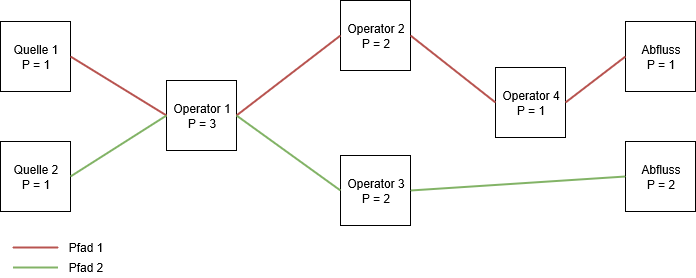
\includegraphics[scale=0.6]{LogischesModell}
\caption{Modell der logischen Topologie}
\end{figure}

In der dargestellten Topologie sind zwei Pfade beschrieben.
Ein Pfad ist durch die Verkettung der Operatoren mit der grünen Linie dargestellt.
Ein Weiterer wird durch die braune Linie beschrieben.
Das erste Element eines Pfades ist die sogenannte Quelle, eine spezielle Form des Operators.
Sie führt Tupel aus einem externen Datenstrom in die Topologie ein.
Tupel sind einzelne Elemente eines Datenstroms, z.B. ein JSON-Objekt.
Das Ende eines Pfads ist immer der Konsument.
Dieser ist der letzte Operator an denen die Tupel aus der Quelle verarbeitet werden. 
Oft werden die Tupel hier an ein anderes System weiter gegeben, in eine Datenbank geschrieben oder auch verworfen.
Die Tupel bewegen sich entlang eines Pfades.

Zwischen der Quelle und dem Abfluss befinden sich weitere Operatoren. 
Diese beinhalten Funktionen, die die Tupel bearbeiten.
Der Operator sendet das Tupel an den nächsten Operator auf dem festgelegten Pfad.
Der nächste Operator wird auch als Nachfolger bezeichnet.
Der Operator, von dem der Operator Tupel empfängt wird als Vorgänger bezeichnet.
So ist Operator 1 der Vorgänger von Operator 2, der wiederum der Nachfolger von Operator 1 ist.
Ein Operator kann, wie in der Abbildung skizziert, auch auf mehreren Pfaden vorhanden sein. 
Allerdings kann ein spezifischer Operator nur einmal innerhalb eines Pfades auftreten, da es sich um einen azyklischen Graph handelt.

In der gezeigten Topologie wird davon ausgegangen, dass Tupel selektiv weitergeleitet werden können.
Das bedeutet, dass ein Operator, welcher sich auf mindestens zwei Pfaden befindet, die Tupel nicht an alle Nachfolger sendet.
Er selektiert stattdessen welche Tupel er an welchen Nachfolger sendet.
Wie in der Abbildung dargestellt sendet Operator 1 die Tupel von Quelle 2 nur an Operator 3 weiter.
Die Tupel von Quelle 1 werden nur an Operator 2 weitergeleitet.
Würden die Tupel jeweils an beide Folgeoperatoren (Operator 2 und Operator 3) weitergeleitet werden, würde die Topologie vier Pfade aufweisen.
Dann beschreibt ein Pfad den Weg von Quelle 1 zu Konsument 2 und der vierte Pfad von Quelle 2 zu Konsument 1.

Alle Operatoren besitzen einen Parallelisierungsgrad, welches direkt den Aufbau des zweiten Graphen bestimmt. 
Der Parallelisierungsgrad ist mindestens eins und kann einen beliebigen aber fixierten Maximalwert nicht überschreiten. 
Die Quelle besitzt laut diesem Modell zwar einen Parallelisierungsgrad, wird jedoch von den nachfolgend implementierten Algorithmen, die die Topologie skalieren, nicht berücksichtigt.
Die Quelle wird in vielen Arbeiten als nicht parallelisierbar modelliert und wird deshalb von vielen Algorithmen nicht betrachtet.************************************

\begin{figure}
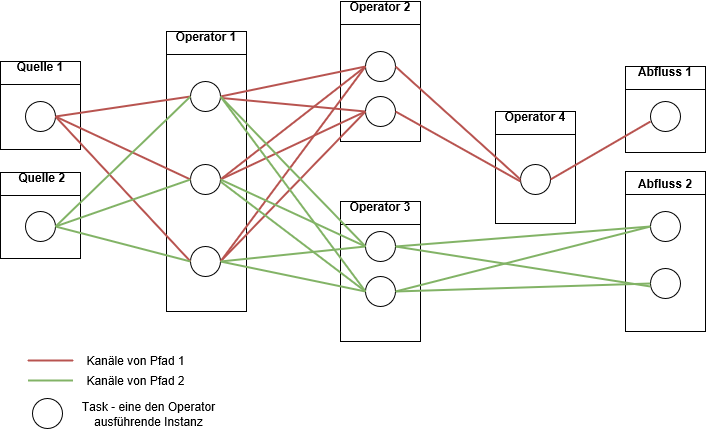
\includegraphics[scale=0.6]{PhysischesModell}
\caption{Modell der physischen Topologie}
\end{figure}

Abbildung 5.2 zeigt die beiden Pfade in der Form, wie sie im CEP-System physisch ausgeprägt sind.
Dies entspricht dem zweiten Graph im vorgestellten Topologie-Modell.
Jeder Operator besitzt genau die Anzahl Tasks, die durch den Parallelisierungsgrad festgelegt ist.
Ein Task ist eine Instanz, welche die Funktion des logischen Operators ausführt.
Zwischen den Tasks befinden sich Kanäle, über die diese miteinander kommunizieren.
Ein Task hat dabei immer einen Kanal zu allen Tasks des folgenden Operators.
So kann ein Tupel von diesem zu jedem beliebigen Task des Nachfolgers gesendet werden.
Die Tasks der Topologie können auf verschiedenen Rechnern verteilt sein und über ein Netzwerk kommunizieren.
Das Modell geht dabei davon aus, das allen Tasks die gleiche Größe von Rechenleistung und Speicher für die Ausführung der Operation zur Verfügung stehen.
Da Quelle und Konsument jeweils die Enden der Topologie darstellen, gibt es keine eingehenden Kanäle an der Quelle sowie keine ausgehenden Kanäle an dem Abfluss.

Wird ein Tupel an den Nachfolger gesendet, so wird es immer nur an einen einzigen Task des Nachfolgers verschickt.
Für die Vorgehensweise wie der Task des Nachfolgers ausgewählt gibt es verschiedene Ansätze.
Dies kann zum einen per Zufall geschehen.
Eine andere Möglichkeit ist das Mapping zu einem bestimmten Task über ein Feld des Tupels.
Eine weitere Möglichkeit ist das Weiterleiten zu einem speziellen Task über einen bestimmten Zeitraum.
Die letzten beiden Methoden sind sinnvoll, wenn der Folgeoperator eine Funkion implementiert die ein Fenster verwendet.
Die Entscheidung, wie die Tupel zwischen Tasks weitergeleitet werden, hat keinen Einfluss auf die selektive Weiterleitung, die zwischen Operatoren auf logischer Ebene definiert ist.

\section{Messwerte}

Um den Datenfluss durch die Topologie zu überwachen, werden Messwerte erfasst.
Diese dienen der Analyse der Topologie als Ganzes und der Untersuchung einzelner Operatoren.
Wenn ein Operator eines Pfads sehr langsam arbeitet, bremst er alle Tupel des gesamten Pfads.
Mit Hilfe der Messwerte können solche Engpässe identifiziert und durch Skalieren des Operators behoben werden.
Die in Kapitel 4 vorgestellten Algorithmen berechnen mit Hilfe der Messwerte den neuen Parallelisierungrad eines Operators.

Das Modell geht davon aus, dass das die gemessenen Werte eines Operators unabhängig von dessen Pfad sind.
Dies bedeutet, dass ein Operator, der auf zwei oder mehr verschiedenen Pfaden liegt, bei den Messwerten nicht zwischen den Pfaden unterscheidet.
Diese Annahme erfordert, dass Tupel unabhängig davon über welchen Pfad sie beim Operator ankommen den gleichen Aufwand beanspruchen.
Sind die Messwerte für die Tasks eines Operators bekannt, kann der Messwert für den Operator aus den Messwerten der Tasks aggregiert werden.
Zähler werden dabei summiert, für die anderen Messwerte der Durchschnitt ermittelt.
Für das Modell werden folgenden Messwerte definiert.
Die Messwerte, die für Tasks beschrieben sind, gelten unter der Annahme, dass sie aggregiert wurden, ebenso für Operatoren.

\begin{itemize}
\item{Pfad-Latenz / Tupel-Latenz: Beschreibt die durchschnittliche Dauer in Millisekunden, die ein Tupel benötigt die Topologie von der Quelle zum Konsumenten zu durchqueren. 
Die Dauer beginnt mit ab der Abgabe des Tupels durch die Quelle bis es vom Konsumenten erfolgreich abgearbeitet wurde. 
Die Messung ist nur zuverlässig, wenn Quelle und Konsument auf dem gleichen Rechner platziert sind, da Uhren verschiedene Rechner nicht zu 100\% synchron sind.}
\item{Fehlgeschlagene Tupel: Gibt die Anzahl Tupel an,  bei denen die Verarbeitung in der Topologie nicht erfolgreich war.
Ursache kann unter anderem ein Fehler während der Bearbeitung durch einen Operator sein.}
\item{Bestätigte Tupel: Anzahl der Tupel, die erfolgreich durch die Topologie abgearbeitet wurden.}
\item{Task-Latenz: Die durchschnittliche Dauer in Millisekunden, die ein Task benötigt um ein Tupel an den nächsten Operator weiter zu geben. 
Diese unterscheidet sich bei Operatoren die ein Fenster verwenden und Operatoren die kein Fenster verwenden  \cite{lohrmann_elastic_2015}.
Ein Fenster beschreibt einen Operators der Tupel aufnimmt, um auf allen gesammelten Tupeln eine Operation durchzuführen.
Meistens erfordert die Operation mehrere Tupel um Zusammenhänge zu erkennen.
Die Latenz des ersten aufgenommenen Tupel ist dann länger als die des Tupels welches zuletzt in das Fenster aufgenommen wurde, da sie alle zusammen wieder weitergeleitet werden wenn das Fenster voll ist. 
Verwendet der Operator kein Fenster, so wird das Tupel direkt nach der Aufnahme verarbeitet und weitergeleitet.
Anschließend wird das nächste Tupel aufgenommen.}
\item{Anzahl Ausführungen des Tasks: Misst die Anzahl wie oft der Task ein neues Tupel aufgenommen und verarbeitet hat.}
\item{Anzahl eingehender Tupel: Misst die Anzahl der Tupel, die beim Task ankommen. Der Messwert ist nicht identisch mit der Anzahl Ausführungen des Tasks, da sich vor dem Task ein Buffer befindet, in dem Tupel zwischengespeichert werden können bevor sie verarbeitet werden.}
\item{Anzahl ausgehender Tupel: Misst die Anzahl der Tupel, die vom Task versendet wurden. Tupel die auf mehreren Pfaden ausgeben werden, werden nicht mehrfach gezählt.}
\item{Abarbeitungsdauer: Beschreibt die durchschnittliche Dauer in Millisekunden, die zwischen dem Aufnehmen von Tupel zur Bearbeitung liegt. 
Die Abarbeitungsdauer ist für Operatoren ohne Fenster gleich der Latenz \cite{lohrmann_elastic_2015}.}
\item{Tupel-Ankunftsintervall: Beschreibt die durchschnittliche Dauer in Millisekunden, die zwischen der Ankunft von zwei Tupeln am Task vergeht.}
\item{Auslastung: Gibt die Auslastung des Tasks in Prozent an. Die Auslastung kann unter anderem durch \(frac{Abarbeitungsdauer}{Tupel-Ankunftsintervall}\) berechnet werden.}
\item{Varianz der Bearbeitungsdauer: Gibt die Varianz der Stichprobe von Messwerten der Bearbeitungsdauer an.}
\item{Varianz des Tupel-Ankunftsintervalls: Gibt die Varianz der Stichprobe von Messwerten des Tupel-Ankunftsintervalls an.}
\item{Latenz des Kanals: Gibt die durchschnittliche Latenz eines Kanals zwischen zwei Tasks in Millisekunden an. 
Die Dauer beginnt ab der Ausgabe des Tupels durch den Vorgänger-Task bis zur Aufnahme des Tupel durch den Nachfolge-Task.
Die Latenz des Kanals beinhaltet insbesondere die Zeit im Ausgangs-Zwischenspeicher des Vorgänger-Task, die Netzwerklatenz und die Zeit im Eingangs-Zwischenspeicher des Nachfolge-Task.}
\item{Latenz der Stapelverarbeitung: Die durchschnittliche Dauer in Millisekunden, die ein Tupel im Ausgangs-Zwischenspeicher des Vorgänger-Task liegt.}
\end{itemize}
\chapter{Implementierung des Frameworks}

Dieses Kapitel beschäftigt sich mit der Architektur und Implementierung des in dieser Arbeit entwickelten Frameworks.
Das Framework schafft eine Abstraktionsebene für die Algorithmen, die die aktiven Topologien in den CEP-Systemen skalieren.
Die reale CEP-Topologie wird in dem Framework als abstrahiertes Graphen-Modell automatisiert erzeugt und den Algorithmen zur Verfügung gestellt.
Dadurch wird ermöglicht, dass Algorithmen, die den Parallelisierungsgrad von Operatoren berechnen, unabhängig vom Zielsystem implementiert werden können.
Anschließend können die implementierten Algorithmen für mehrere verschiedene CEP-Systeme eingesetzt werden, ohne dass Anpassungen am Algorithmus vorgenommen werden müssen.
Außerdem skaliert das Framework automatisch die einzelnen Operatoren mit den berechneten Parallelisierungsgraden.
Die vorliegende Architektur ermöglicht die zeitgleiche Steuerung mehrerer CEP-Topologien, die auch über diverse CEP-Systeme verteilt werden können.

Im Folgenden werden die einzelnen Komponenten des Frameworks und ihre Funktion erläutert.
Außerdem werden die Abhängigkeiten zwischen den Komponenten dargestellt.
Anschließend wird noch speziell auf die Messwerte eingegangen, die im Graphen-Modell des Frameworks vorgehalten werden.
 

\section{Architektur}

Die Architektur des Frameworks besteht aus mehreren Komponenten und verfolgt zwei Ziele.
Eines der beiden Hauptziele der Architektur ist, dass das System einfach um weitere Algorithmen erweitert werden kann.
Um dieses Ziel zu erreichen, wurde eine Abstraktionsebene eingeführt, die die Eigenschaften der realen CEP-Topologie repräsentiert.
Diese Abstraktion wird durch ein Graphen-Modell repräsentiert, das einen gerichteten, azyklischen Graphen modelliert.
Die implementierten Algorithmen arbeiten ausschließlich auf dem abstrahierten Modell.
Für die Implementierung eines neuen Algorithmus, müssen nur die Daten aus dem Modell ausgelesen und anschließend verarbeitet werden.
Außerdem ist es möglich mehrere Algorithmen für das gleiche Modell auszuführen und ihre Ergebnisse zu vergleichen.
Um einen Algorithmus für das System zu implementieren ist ausschließlich Wissen über das Modell notwendig.

Ein weiteres Ziel ist, dass das System für weitere CEP-Systeme außer Heron verwendet werden kann.
Dazu wurde eine API, die bereits in einer vorhergehenden Bachelorarbeit entwickelt wurde, erweitert \cite{goggel_vergleich_2018}.
Alle Komponenten des Systems benutzen diese API für die Kommunikation mit dem CEP-System, sodass diese alle system-spezifischen Befehle abstrahieren kann.
Die Seite der API, die mit dem System direkt kommuniziert, ist ein eigenständiger Adapter.
Dieser Adapter wird auf dem Rechner installiert, der das zu steuernde CEP-System kontrolliert.
Der Adapter ist über eine REST-API ansprechbar.
Somit kann das Framework auf einem eigenständigen Rechner installiert werden und das Zielsystem über die REST-Schnittstelle des Adapters kontrollieren.
Dies ermöglicht die Kontrolle von mehreren CEP-Systemen zur gleichen Zeit.
Das Framework kann durch die Implementierung eines entsprechenden Adapters für weitere CEP-Systeme erweitert werden.
Um einen neuen Adapter zu erstellen ist ausschließlich Wissen über die Spezifikation der REST-Schnittstelle notwendig.
Das Framework kann so über die REST-API verschiedene CEP-Systeme über eine einheitlichen Schnittstelle ansprechen.

Die Architektur des Systems ist in der Abbildung 5.1 dargestellt.
Im Folgenden werden die einzelnen Komponenten der Architektur genauer erläutert.

\begin{figure}
  \centering
  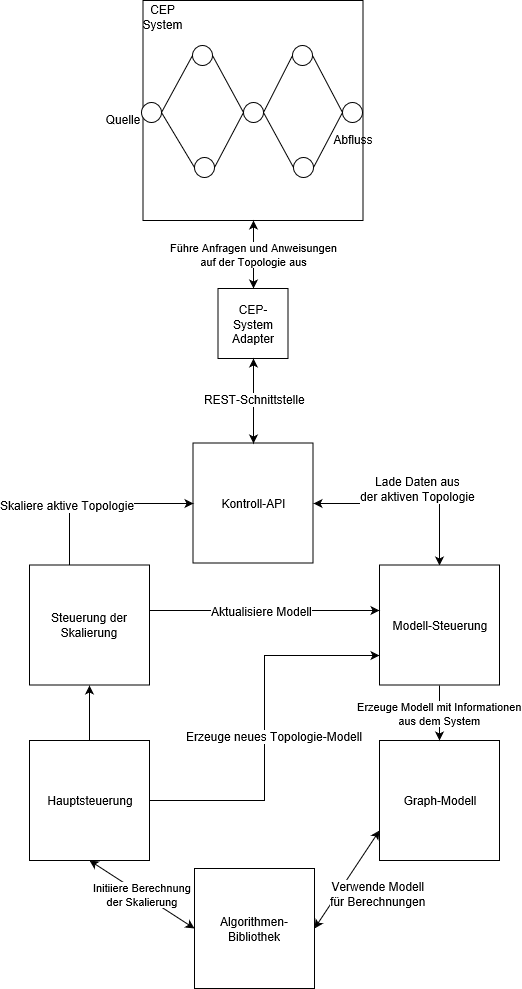
\includegraphics[scale=0.65]{Systemaufbau.png}
  \caption{Architektur des Frameworks}
  \label{fig:Architektur}
\end{figure}

\section{Graphen-Modell}
Das Graphen-Modell repräsentiert die Topologie im realen CEP-System.
Alle Elemente der Topologie werden nach dem in Kapitel vier vorgestellten Topologie-Modell abgebildet.
Es dient als Cache für Messdaten aus dem realen System.
Durch die Zwischenspeicherung wird ermöglicht, dass ein Modell eines bestimmten Zeitpunktes des realen Systems zur Verfügung gestellt werden kann. 
Würden die Algorithmen die Werte zur Laufzeit abfragen, also immer dann, wenn die Werte benötigt werden, kann dies zu einem inkonsistenten Modell führen.
Die Algorithmen verwenden das Modell, um die Inkosistenz von Messungen zu verschiedenen Zeitpunkten zu verhindern.

Jedes Modell besteht aus Pfaden und Operatoren.
Jeder Pfad stellt dabei eine geordnete Folge von Operatoren dar.
Das Modell erlaubt kreuzende Pfade, sodass Operatoren in mehreren Pfaden verwendet werden können.
Operatoren sind über einen Namen identifizierbar und haben eine dem Parallelisierungsgrad entsprechende Anzahl an Tasks.
Sobald der Operator einen neuen Parallelisierungsgrad erhält, wird die entsprechende Anzahl Tasks gelöscht oder erzeugt.
Somit ist die Anzahl Tasks immer gleich dem Parallelisierungsgrad des Operators.
Der maximale und minimale Parallelisierungsgrad aller Operatoren kann über zwei Konstanten angegeben werden. 
Diese gelten für alle Operatoren in allen Modellen. 
Ein logisch schlüssiger Minimalwert ist ein Parallelisierungsgrad von eins.
Ein Parallelisierungsgrad kleiner als eins ist für einen aktiven Operator nicht gültig, da er keinen ausführenden Task besitzt.
Das Maximum kann entsprechend der Ressourcen, die im CEP-System zur Verfügung stehen, angepasst werden.
Somit kann über Pfade und Operatoren die logische Struktur der Topologie im Modell dargestellt werden.

Die ausführende Ebene, oder physische Struktur, wird durch Tasks und Kanäle repräsentiert.
Tasks sind die Recheninstanzen, die die Operation eines Operators auf Tupel ausführen.
In der vorliegenden Implementierung des Graphen-Modells ist die Zwischenspeicherung der Messwerte auf Task-Ebene vorgesehen.
Somit wird ermöglicht, dass ein detailliertes Modell der Topologie im Frameowork erzeugt werden kann.
Die Kennung der Tasks wird vom Operator automatisch erzeugt.
Sie wird aus dem Namen des Operators und einer fortlaufenden Nummer wie folgt gebildet: \textit{<Name>\_<Nummer>}.
Die niedrigste Nummer ist immer die eins.
Die höchste Nummer entspricht immer dem aktuellen Parallelisierungsgrad des Operators.
Für Tasks sind folgende Messwerte in der aktuellen Version des Modells vorgesehen:

\begin{itemize}
\item{Task-Latenz}
\item{Anzahl Ausführungen des Tasks}
\item{Anzahl eingehender Tupel}
\item{Anzahl ausgehender Tupel}
\item{Auslastung}
\item{Bearbeitungsdauer}
\item{Tupel-Ankunftsintervall}
\item{Varianz der Bearbeitungsdauer}
\item{Varianz des Tupel-Ankunftsintervalls}
\end{itemize}

Wie in Kapitel vier beschrieben wird für die Messwerte der Tasks die Annahme getroffen, dass sie unabhängig vom Pfad sind.
Dies bedeutet zum Beispiel, dass alle eingehenden Tupel durchschnittlich die selbe Bearbeitungsdauer benötigen.
Unabhängig davon von welchem vorhergehenden Operator sie stammen.
Alle für den Task erfassten Metriken differenzieren nicht die Herkunft der Tupel, sondern erfassen sie gesammelt.

Für viele Algorithmen wird nicht der Messwert eines einzelnen Tasks betrachtet, jedoch können die Werte gemittelt beziehungsweise summiert werden um einen aussagekräftigen Messwert für den gesamten Operator zu bekommen.
Um die Messwerte für Operatoren zu berechnen ist pro Messwert eine statische Methode im Modell implementiert.

Die Kommunikation zwischen den Tasks wird durch die Kanäle repräsentiert.
Diese speichern Metriken der Kommunikationskanäle zwischen Tasks.
Für die Implementierung des Modells wurde die Annahme getroffen, dass alle Tasks eines Operators mit allen Tasks der vorhergehenden und nachfolgenden Operatoren kommunizieren können.
Die Anzahl an Kanälen zwischen zwei Operatoren ist also das Produkt aus deren Parallelisierungsgraden.
Für Kanäle sind folgende Messwerte vorgesehen:

\begin{itemize}
\item{Latenz des Kanals}
\item{Latenz der Stapelverarbeitung}
\end{itemize}

Details zu den Messwerten werden in Kapitel 4 erläutert.

\section{Modell-Steuerung}

Die Modell-Steuerung erzeugt die Modellstruktur der Topologien und füllt diese anschließend mit Messwerten.
Alle Aktionen werden von der Hauptsteuerung initiiert.
Im ersten Schritt wird die Topologie vom CEP-System über die Kontroll-API ausgelesen.
Welche Topologie ausgelesen wird entscheidet die angegebene Adapteradresse.
Ein Adapter ist jeweils für eine Topologie zuständig.
Zuerst werden die Pfade der Topologie ausgelesen und im Graphen-Modell die entsprechenden Operatoren und Pfade angelegt.
Dann wird der Parallelisierungsgrad der Operatoren gesetzt.
Wie zuvor beschrieben erzeugen dies durch das Setzen des Parallelisierungsgrades die entsprechende Anzahl an Tasks und Kanälen.
Damit ist das leere Graphen-Modell der Ziel-Topologie erstellt.

Anschließend erzeugt die Modell-Steuerung eine Zuweisung von Tasks im realen System zu den Tasks im Modell.
Die Tasks im Modell sind, wie im vorherigen Kapitel beschrieben, durchnummeriert und haben einen durch das Graphen-Modell festgelegten Namen.
Diese Namen weichen sehr wahrscheinlich von den Namen im realen CEP-System ab.
Damit nun die Messwerte eines realen Tasks konsistent einem modellierten Task zugewiesen werden können, wird pro Operator eine Zuweisungstabelle für die Tasks erzeugt.
Diese Zuweisung muss mit jeder Änderung des Parallelisierungsgrades des Operators angepasst werden, da Tasks wegfallen oder hinzu kommen.
Ist die Zuweisung erfolgt werden zuletzt die Messwerte über die Kontroll-API in das Modell geladen.

\section{Steuerung der Skalierung}

Die Steuerung der Skalierung übernimmt zwei Aufgaben.
Zum Einen werden die Ergebnisse der ausgeführten Algorithmen an das CEP-System geben.
Dazu wird die Kontroll-API verwendet.
Der Adapter passt die Parallelisierungsgrade in der aktiven Topologie an.
Nachdem die reale Topologie erfolgreich angepasst ist wird im zweiten Schritt das Modell angepasst.
Hier werden ebenfalls die neuen Parallelisierungsgrade, die durch den Algorithmus berechnet wurde, gesetzt.
Die Komponente übernimmt somit die Steuerung der Parallelisierungsgrade im Modell und im realen System.

\section{Hauptsteuerung}

Die Hauptsteuerung ist die zentrale Steuereinheit des Frameworks.
Sie enthält die Logik, die die anderen Komponenten kontrolliert und die zuvor beschriebenen Abläufe steuert.
Sie instanziiert die anderen Komponenten für jede Topologie, die gesteuert werden soll.
Außerdem werden die Parameter definiert, die für Berechnungen in den Algorithmen verwendet werden.
Die zeitliche Abfolge aller Abläufe zu steuern ist die Kernaufgabe der Komponente.

\section{Kontroll-API}

Die Kontroll-API abstrahiert die APIs der verschiedenen CEP-Systeme.
Grundsätzlich besteht Sie aus zwei Teilen.
Ein Teil nimmt die Aufrufe aus dem Framework entgegen und wandelt sie in REST-Anfragen um.
Die Anfragen werden anschließend an den entsprechenden Adapter gesendet.
So wird die REST-Schnittstelle über die zur Verfügung gestellten Funktionen gekapselt.
Dieser Teil ist auf der gleichen Maschine wie die anderen Komponenten des Frameworks und wird direkt von den anderen Komponenten angesprochen.

Der zweite Teil, der Adapter, befindet sich auf der Maschine des zu steuernden CEP-Systems.
Er nimmt REST-Anfragen entgegen und setzt diese in Befehle für die API des CEP-Systems um.
Der Adapter ist somit der Teil, der das Kontroll-Schnittstelle des CEP-Systems auf eine einheitliche REST-Schnittstelle abstrahiert.
Außerdem kapselt der Adapter die zurückgelieferten Messwerte des CEP-Systems und vereinheitlicht sie für das Graphen-Modell.
Deshalb ist die Implementierung des Adapters essentiell für die Qualität des Graphen-Modells.
Die Implementierung des Adapters für das CEP-System Heron wird in Kapitel sechs ausführlich behandelt.

Die Kommunikation über die REST-API ermöglicht es, dass die beiden teile auf verschiedenen Maschinen installiert sein können.
Durch die Fern-Steuerung über die Schnittstelle können mit einer einzelnen Installation des Frameworks mehrere CEP-Systeme und Topologien gleichzeitig gesteuert werden.




















\chapter{Adapter für Heron}

Wie bereits in der Architektur des Frameworks beschrieben, stellt der Adpater die Komponente dar, die eine uniforme Steuerung verschiedener CEP-Systeme ermöglicht.
Der Adapter kapselt die spezifischen Eigenschaften eines CEP-Systems und dessen Kontroll-Schnittstelle.
Die Funktionen des Adapters werden über eine einheitliche REST-Schnittstelle veröffentlicht.
So können von einer zentralen Installation des Frameworks mehrere Adapter über das Netzwerk mit dem HTTP-Protokoll angesprochen werden.
Dies ermöglicht die unabhängige Platzierung von CEP-Systemen und des Frameworks.
Der Adapter wird normalerweise auf dem Rechner platziert, auf dem die Steuer-Komponente des CEP-Systems liegt.
Allerdings muss dies je nach Art der Kontroll-Schnittstelle des CEP-Systems nicht zwingend notwendig sein.
Das folgende Kapitel befasst sich mit der Umsetzung des Adapters für das CEP-System Heron.

Die beschriebene Architektur des Adapters wurde von der bestehenden Version übernommen \cite{goggel_vergleich_2018}.
Allerdings wurden alle Funktionen der aktuellen Version des Adapters entweder neu hinzugefügt oder angepasst.

\section{Implementierung}

Das Ziel des Adapters ist eine bestimmte Topologie im System ansprechen zu können.
Ein Adapter ist daher immer nur für eine spezifische Topologie zuständig.
Diese Entscheidung wurde zur Vereinfachung der REST-API getroffen.
So müssen nicht bei jedem Aufruf alle Parameter angegeben werden, die eine spezifische Topologie identifizieren.
Die korrekte IP-Adresse und der korrekte Port genügen um den Adapter für eine Topologie anzusprechen.
Außerdem können die Merkmale, die eine Topologie identifizieren, bei unterschiedlichen CEP-Systemen variieren.
Bei variierenden Merkmalen zur Identifizierung ist es nicht möglich eine einheitliche Schnittstelle zu erzeugen.
Mit der gewählten Architektur können die Merkmale beim Start des Adapter angegeben werden.
Jede Implementation eines Adapters kann die Start-Parameter beliebig festlegen und bietet somit Flexiblität für die Definition der Topologie.
Es ist aber möglich mehrere Adapter auf unterschiedlichen Ports zu starten um mehrere Topologien des selben CEP-Systems ansprechen zu können.

Um den Adapter für Heron zu Starten werden folgende Parameter benötigt:
\begin{itemize}
\item{URL: Definiert die Adresse unter der die REST-Schnittstelle erreichbar ist.}
\item{Tracker URL: Definiert die Adresse unter der die REST-API von Heron erreichbar ist.}
\item{Cluster: Bestimmt den Cluster in dem die Ziel-Topologie ausgeführt wird.}
\item{Topologie: Der Name mit dem die Topologie identifiziert wird.}
\item{Umgebung: Wird von Heron ebenfalls benutzt um die Topologie zu identifizieren.}
\item{Heron CLI: Spezifiziert den Pfad zu den ausführbaren Programmen von Heron.}
\item{CLI Clustername: Spezifiziert wie das Cluster über die CLI angesprochen werden kann.}
\item{Messwert-Interval: Definiert die Zeitspanne der Messwerte, die ausgelesen werden, in Sekunden.}
\end{itemize}
Der Adapter ist in eine eigenständige JAR-Datei verpackt, die auf jedem Rechner mit installierter Java Laufzeitumgebung ausgeführt werden kann.
Beim Ausführen wird ein glassfish-Server gestartet.
Dieser nimmt Anfragen an die REST-Schnittstelle entgegen.

Werden über die REST-Schnittstelle Messwerte oder der Aufbau der Topologie angefragt, leitet der Adapter die Anfrage an Heron weiter.
Heron bietet für die Abfrage von Messwerten selbst eine REST-Schnittstelle an.
Die Implementation des Adapters kapselt die REST-Schnittstelle von Heron und abstrahiert sie.
Messwerte werden immer für die in den Startparametern definierte Topologie abgefragt.
Wie Metriken von Heron bereit gestellt und wie diese vom Adapter angepasst werden ist im folgenden Kapitel detailliert ausgeführt.

\section{Messwerte in Heron}

Ein essentieller Teil des Adapters ist die Anpassung der vom CEP-System gelieferten Messwerte an die im Graphen-Modell erwarteten Werte.
CEP-Systeme erfassen Messwerte auf unterschiedliche Arten oder legen unterschiedliche Messpunkte für den Wert fest.
Das Wissen, wie CEP-Systeme die Messwerte erfassen, muss durch den Adapter gekapselt werden.
Die Annahmen, die das Graphen-Modell trifft, werden in Kapitel 4 diskutiert.

Heron arbeitet mit einem verteilen System für die Erfassung der Messdaten.
Alle Container, die einen Task enthalten, sammeln die Messwerte autonom.
Jede Minute werden die Werte von den einzelnen Containern zu einer zentralen Einheit, dem sogenannten Metrik-Manager, gesendet.
Dieser sammelt die Daten und sichert sie zentral für die Bedienung der Anfragen.

Auf der Webseite von Heron wird angegeben dass die erfassten Messwerte bis zu drei Stunden vorgehalten werden \cite{noauthor_heron_nodate}.
Alle Werte die vor dieser Zeitspanne erfasst wurden sind nicht mehr verfügbar.
Die Messwerte von Heron werden in einer Auflösung von einer Minute erfasst und gesichert.
Die Messwerte können von Heron als Zeitreihe mit der Auflösung von einer Minute abgefragt werden.
Alternativ können die Messwerte von Heron direkt aggregiert abgerufen werden.
Da das Graph-Modell nur aggregierte Messwerte und keine Zeitreihen unterstützt, werden vom Adapter direkt die aggregierten Messwerte abgefragt.

Der Parameter Messwert-Intervall, der definiert werden muss um den Adapter zu starten, bestimmt die Zeitspanne für die die Messwerte aggregiert werden.
Der Endzeitpunkt der Spanne ist immer der Zeitpunkt t, an dem der Adapter die Anfrage an Heron sendet.
Wenn der Parameter Messwert-Intervall durch s repräsentiert wird, so werden alle Werte die in der Zeitspanne \([t-s, t]\) liegen aggregiert.

Heron bietet über die REST-API standardmäßig die untenstehenden, auf Operatoren bezogenen Messwerte an.
Die Art der Messwerte unterscheidet sich bei Quell-Operatoren und anderen verarbeitenden Operatoren.
Betrachten wir zuerst die Quell-Operatoren:

\begin{itemize}
\item{\_\_ack-count: Dieser Wert beschreibt die Anzahl an Tupel, die durch das CEP-System bereits als erfolgreich abgearbeitet an den Quell-Operator zurückgemeldet wurden. 
Dieser Messwert wird nur erfasst, falls die Topologie für die Bestätigung der Tupel konfiguriert und implementiert ist.}

\item{\_\_fail-count: Dieser Wert gibt die Anzahl an Tupel an, bei denen während der Verarbeitung Fehler aufgetreten sind. Tritt ein Fehler auf wird dies bei entsprechender Implementation an den Quell-Operator gemeldet. Dieser Messwert wird nur gemessen, falls die Topologie für die Bestätigung der Tupel konfiguriert und implementiert ist.}

\item{\_\_emit-count: Gibt die Anzahl von Tupel an, die von dem Quell-Operator ausgegeben wurden.}

\item{\_\_complete-latency: Gibt die Tupel-Latenz für eine erfolgreiche Bearbeitung eines Tupels in der Topologie an. Dieser Wert kann von der Quelle berechnet werden, wenn die erfolgreiche Verarbeitung des Tupels zurückgemeldet wird.}

\end{itemize}

Verarbeitende Operatoren:

\begin{itemize}
\item{\_\_execute-count: Jeder verarbeitende Operator besitzt eine Methode, die von Heron aufgerufen wird und ankommende Tupel verarbeitet. Dieser Wert gibt an, wie oft die verarbeitende Methode aufgerufen wurde. Dieser Messwert gibt keine Aussage über die Anzahl ausgegebener Tupel.}

\item{\_\_ack-count: In der Methode, die die Tupel verarbeitet, kann zu einem beliebigen Zeitpunkt die erfolgreiche Verarbeitung des Tupels an den Quell-Operator signalisiert werden. Dieser Messwert gibt die Anzahl der Tupel an, die von diesem Operator an den Quell-Operator als erfolgreich verarbeitet zurückgemeldet wurden.}

\item{\_\_fail-count: Ebenso kann in der Methode, die die Tupel verarbeitet, das Auftreten eines Fehlers an den Quell-Operator signalisiert werden. Der Zeitpunkt der Benachrichtigung ist wiederum vollständig von der Implementierung der Methode abhängig. Der Messwert gibt die Anzahl der an den Quell-Operator signalisierten Fehler an.}

\item{\_\_execute-latency: Dieser Messwert beschreibt die durchschnittliche Laufzeit der Methode, die die Tupel verarbeitet, in Nanosekunden. Ein Tupel kann zu jedem beliebigen Zeitpunkt der Methode ausgegeben werden. Tupel können auch an mehreren Zeitpunkten während der Ausführung der Methode ausgegeben werden. Dies bedeutet, dass dieser Messwert nicht zwingend die Dauer bis zur Ausgabe des Tupels darstellt. Dies trifft ebenso für die Benachrichtigungen über Erfolg oder Fehlschlag an den Quell-Operator zu. Ob der Messwert für die Latenz des Tupels im Operator aussagekräftig ist, hängt von der Implementation des Operators ab.}

\item{\_\_process-latency: Dieser Wert gibt die Dauer in Nanosekunden an, die benötigt wurde um die Verarbeitung eines Tupels als erfolgreich oder fehlerhaft zu melden. Er misst jedoch nicht die Latenz des Tupels im Operator. Gemessen wird ausschließlich die Zeit von Beginn der verarbeitenden Methode bis zu dem Zeitpunkt, an dem die Benachrichtigung, ob das Tupel erfolgreich verarbeitet oder fehlerbehaftet war, erzeugt wird. Die Rückmeldung innerhalb der Methode kann, wie oben beschrieben, zu einem beliebigen Zeitpunkt während der Ausführung geschehen.}

\item{\_\_emit-count: Gibt die Anzahl von Tupel an, die von dem verarbeitenden Operator ausgegeben wurden.}

\end{itemize}

Eine exakte Definition der Messwerte, die von Heron erfasst werden, ist dem momentanen Stand der Heron-Dokumentation nicht immer zu entnehmen. 
Deshalb wurde die Bedeutung, der von Heron bereitgestellten Messwerte, empirisch festgestellt.

Alle vorangegangenen Ausführungen beziehen sich auf die Standardeinstellungen von Heron in der Version 17.05.
Alle Konfigurationen können in den Files \textit{metrics\_sinks.yaml} und \textit{heron\_internals.yaml} in dem Verzeichnis des verwendeten Clusters angepasst werden. 
Außerdem bietet Heron die Möglichkeit Messdaten in Drittsysteme zu exportieren.
Somit bietet sich die Möglichkeit für Algorithmen, die auf Basis von bestehenden Daten das Verhalten der Topologie erlernen, Messdaten länger aufzubewahren.

\section{REST-Schnittstelle}

Welche Funktionen der Adapter implementieren muss, wird durch die REST-Schnittstelle festgelegt.
Im Detail implementiert der Adapter ein Java Interface.
Der glassfish-Server veröffentlicht dann die im Interface definierten Methoden über die REST-Schnittstelle.
Die Schnittstelle stellt für jeden Messwert im Graph-Modell eine Methode bereit, über die der Wert ausgelesen werden kann.
Anfragen werden von der Schnittstelle mit JSON-Objekten beantwortet.
Die vollständige Dokumentation der REST-Schnittstelle ist Tabelle 6.1 zu entnehmen.


Betrachtet man die standardmäßig von Heron gelieferten Messwerte im vorherigen Kapitel, so ist ersichtlich, dass Heron nicht alle benötigten Messwerte für die REST-Schnittstelle liefert.
Deshalb verlangt die Implementation des Adapters, dass die fehlenden Werte bestmöglich approximiert werden.

Sämtliche Latenzen werden vor der Weitergabe über die Schnittstelle auf Millisekunden umgerechnet.
Heron unterstützt des Weiteren nur die Task-Latenz jedoch nicht die Bearbeitungsdauer.
Bei der Verwendung von Fenster-Operatoren kann es zu fehlerhaften Messwerten kommen, da als Bearbeitungsdauer die Task-Latenz angenommen werden muss.
Wie in Kapitel vier beschrieben ist die hier getroffene Annahme, dass die Task-Latenz gleich der Bearbeitungsdauer ist, nur für Operatoren ohne Fenster gültig.

Ein weiterer Punkt ist die Anzahl eingehender Tupel am Operator.
Dieser Messwert wird in Heron nicht erfasst.
Daher wird für die Implementation des Operators angenommen, dass die Anzahl ausgehender Tupel des Vorgängers gleich der Anzahl eingehender Tupel am betrachteten Operator sind.

Die Varianzen der jeweiligen Werte werden mit Hilfe der von Heron gelieferten Zeitreihe berechnet.
Die Größe der Stichprobe ist die Anzahl der minütlichen Werte, die von Heron geliefert werden.
Sie ist somit von dem gewählten Messwert-Intervall abhängig.

\begin{longtable}{|p{2cm}|p{12cm}|}

\caption{Operationen der REST-Schnittstelle}
\endfirsthead
\caption{Operationen der REST-Schnittstelle}
\endhead
\endfoot
\endlastfoot

\hline
Operation & /v1/getalloperators \\ \hline
Ergebnis & {[}''Operator1'', ''Operator3'', ''Operator2''{]} \\ \hline
Beschreibung & Liefert alle Operatoren unsortiert in einem Array mit Strings zurück \\ \hline
\multicolumn{2}{|l|}{} \\ \hline

Operation & /v1/getlogicaltopology \\ \hline
Ergebnis & \{''Pfad1'':{[}''Operator1'',''Operator3''{]}, ''Pfad2'':{[}''Operator1'',''Operator2''{]}\} \\ \hline
Beschreibung & Liefert alle Pfade der Topologie als Objekt zurück. Jedes Objekt besitzt ein Array mit den Operatoren in korrekter Reihenfolge \\ \hline
\multicolumn{2}{|l|}{} \\ \hline

Operation & /v1/getoperatorparallelism?operator=Operator3 \\ \hline
Ergebnis & 4 \\ \hline
Beschreibung & Liefert den Parallelisierungsgrad des Operators als Integer \\ \hline
\multicolumn{2}{|l|}{} \\ \hline

Operation & /v1/getpathlatency?operator=Operator1 \\ \hline
Ergebnis & 80.3 \\ \hline
Beschreibung & Liefert die durchschnittliche Latenz der Pfade, bei denen der Operator die Quelle ist, als Gleitkommazahl in Millisekunden zurück. Die Operation ist nur für Quell-Operatoren erlaubt.  \\ \hline
\multicolumn{2}{|l|}{} \\ \hline

Operation & /v1/getfailedtuplescount?operator=Operator1 \\ \hline
Ergebnis & 0.0 \\ \hline
Beschreibung & Liefert die Anzahl der Tupel, bei denen der Operator die Quelle und die Verarbeitung fehlgeschlagen ist. Die Operation ist nur für Quell-Operatoren erlaubt.  \\ \hline
\multicolumn{2}{|l|}{} \\ \hline

Operation & /v1/getackedtuplescount?operator=Operator1 \\ \hline
Ergebnis & 100000.0 \\ \hline
Beschreibung & Liefert die Anzahl der Tupel, bei denen der Operator die Quelle ist und erfolgreich bearbeiten wurden. Die Operation ist nur für Quell-Operatoren erlaubt.  \\ \hline
\multicolumn{2}{|l|}{} \\ \hline

Operation & /v1/getlatency?operator=Operator2\&operation=AVG \\ \hline
Ergebnis & 5.615 \\ \hline
Beschreibung & Liefert die Latenz des Operators als Gleitkommazahl in Millisekunden. Dazu werden die Werte der einzelnen Tasks aggregiert. Erlaubte Operationen sind AVG, SUM, MAX, MIN. Die Operation ist für Quell-Operatoren nicht erlaubt \\ \hline
\multicolumn{2}{|l|}{} \\ \hline

Operation & /v1/getoperatorlatency?operator=Operator2 \\ \hline
Ergebnis & \{''Task1'':5.32, ''Task2'':5.01\} \\ \hline
Beschreibung & Liefert ein Objekt, das die Tasks des Operators beinhaltet. Jeder Task hat als Wert die Latenz des Tasks als Gleitkommazahl zugewiesen. Die Operation ist für Quell-Operatoren nicht erlaubt. \\ \hline
\multicolumn{2}{|l|}{} \\ \hline

Operation & /v1/getoperatorlatencyvariance?operator=Operator2 \\ \hline
Ergebnis & \{''Task1'':3.33, ''Task2'':3.87\} \\ \hline
Beschreibung & Liefert ein Objekt, das die Tasks des Operators beinhaltet. Jeder Task hat als Wert die Varianz der Latenz des Tasks als Gleitkommazahl zugewiesen. Die Operation ist für Quell-Operatoren nicht erlaubt. \\ \hline
\multicolumn{2}{|l|}{} \\ \hline

Operation & /v1/getoutputcount?operator=Operator1\&operation=SUM \\ \hline
Ergebnis & 100000.0 \\ \hline
Beschreibung & Liefert die Anzahl der Tupel, die der Operator ausgegeben hat. Dazu werden die Werte der einzelnen Tasks aggregiert. Erlaubte Operationen sind AVG, SUM, MAX, MIN. \\ \hline
\multicolumn{2}{|l|}{} \\ \hline

Operation & /v1/getoperatoroutputcount?operator=Operator1 \\ \hline
Ergebnis & \{''Task1'':50000, ''Task2'':50000\} \\ \hline
Beschreibung & Liefert ein Objekt, das die Tasks des Operators beinhaltet. Jeder Task hat als Wert die Anzahl der Tupel, die der Task ausgegeben hat, zugewiesen. \\ \hline
\multicolumn{2}{|l|}{} \\ \hline

Operation & /v1/getoperatoroutputcountvariance?operator=Operator1 \\ \hline
Ergebnis & \{''Task1'':3.33, ''Task2'':3.87\} \\ \hline
Beschreibung & Liefert ein Objekt, das die Tasks des Operators beinhaltet. Jeder Task hat als Wert die Varianz der Tupel, die der Task ausgegeben hat, als Gleitkommazahl zugewiesen. \\ \hline
\multicolumn{2}{|l|}{} \\ \hline

Operation & /v1/getexecutioncount?operator=Operator2\&operation=SUM \\ \hline
Ergebnis & 100000.0 \\ \hline
Beschreibung & Liefert zurück wie oft der Operator ausgeführt wurde. Dazu werden die Werte der einzelnen Tasks aggregiert. Erlaubte Operationen sind AVG, SUM, MAX, MIN. Die Operation ist für Quell-Operatoren nicht erlaubt. \\ \hline
\multicolumn{2}{|l|}{} \\ \hline

Operation & /v1/getoperatorexecutioncount?operator=Operator2 \\ \hline
Ergebnis & \{''Task1'':50000, ''Task2'':50000\} \\ \hline
Beschreibung & Liefert ein Objekt, das die Tasks des Operators beinhaltet. Jeder Task hat als Wert die Anzahl wie oft der Task ausgeführt wurde. Die Operation ist für Quell-Operatoren nicht erlaubt. \\ \hline
\multicolumn{2}{|l|}{} \\ \hline

Operation & /v1/getoperatorexecutioncountvariance?operator=Operator2 \\ \hline
Ergebnis & \{''Task1'':3.33, ''Task2'':3.87\} \\ \hline
Beschreibung & Liefert ein Objekt, das die Tasks des Operators beinhaltet. Jeder Task hat als Wert die Varianz der Anzahl wie oft der Task ausgeführt wurde als Gleitkommazahl zugewiesen. Die Operation ist für Quell-Operatoren nicht erlaubt. \\ \hline
\multicolumn{2}{|l|}{} \\ \hline

Operation & /v1/getinputcount?operator=Operator2\&operation=SUM \\ \hline
Ergebnis & 100000.0 \\ \hline
Beschreibung & Liefert die Anzahl der Tupel, die beim Operator angekommen sind. Dazu werden die Werte der einzelnen Tasks aggregiert. Erlaubte Operationen sind AVG, SUM, MAX, MIN. Die Operation ist für Quell-Operatoren nicht erlaubt.\\ \hline
\multicolumn{2}{|l|}{} \\ \hline

Operation & /v1/getoperatorinputcount?operator=Operator2 \\ \hline
Ergebnis & \{''Task1'':50000, ''Task2'':50000\} \\ \hline
Beschreibung & Liefert ein Objekt, das die Tasks des Operators beinhaltet. Jeder Task hat als Wert die Anzahl der Tupel, die beim Task angekommen sind, zugewiesen. Die Operation ist für Quell-Operatoren nicht erlaubt.\\ \hline
\multicolumn{2}{|l|}{} \\ \hline

Operation & /v1/getoperatorinputcountvariance?operator=Operator2 \\ \hline
Ergebnis & \{''Task1'':3.33, ''Task2'':3.87\} \\ \hline
Beschreibung & Liefert ein Objekt, das die Tasks des Operators beinhaltet. Jeder Task hat als Wert die Varianz der Tupel, die beim Task angekommen sind, als Gleitkommazahl zugewiesen. Die Operation ist für Quell-Operatoren nicht erlaubt. \\ \hline
\multicolumn{2}{|l|}{} \\ \hline

Operation & /v1/setoperatorparallelism?operator=Operator2?parallelism=4 \\ \hline
Ergebnis & true \\ \hline
Beschreibung & Setzt den Parallelisierungsgrad des Operators auf den definierten Wert. Liefert true wenn der Vorgang erfolgreich war, false wenn nicht. \\ \hline
\multicolumn{2}{|l|}{} \\ \hline

Operation & /v1/setmultipleoperatorparallelism?map=Operator2:4;Operator3:2 \\ \hline
Ergebnis & true \\ \hline
Beschreibung & Setzt den Parallelisierungsgrad der Operatoren auf den definierten Wert. Liefert true wenn der Vorgang erfolgreich war, false wenn nicht. \\ \hline
\multicolumn{2}{|l|}{} \\ \hline

\end{longtable}









\chapter{Algorithmus mit Warteschlangen-Theorie}

Lohrmann et al. beschreiben in ihrem Paper \cite{lohrmann_elastic_2015} einen Algorithmus, der das Ziel verfolgt, die Latenz der Tupel einer Topologie unter einem, durch den Benutzer bestimmten, Maximalwert zu halten.
Dieses Ziel soll mit einem möglichst geringen Verbrauch von Ressourcen erreicht werden.
Die Latenz eines Tupels bestimmt sich aus der Zeit, welche das Tupel benötigt um von der Quelle zum Konsument zu gelangen.

Dementsprechend ist die Wahl des Pfades für die Latenz des Tupels essentiell, da die sie mindestens die Summe der Latenz aller Operatoren in einem Pfad ist.
Außerdem fließt die Zeit, in der Tupel sich zwischen Operatoren bewegen, in die Latenz des Tupels mit ein.
Einerseits beinhaltet dies die Latenz des Netzwerks, über das die Tupel versendet werden.
Diese Latenz kann jedoch nicht durch reines Skalieren der Operatoren beeinflusst werden, sondern ist von deren Platzierung abhängig.
Im Modell des Algorithmus wird die Netzwerklatenz nicht explizit berücksichtigt.
Der zweite Faktor ist die Zeit, welche zwischen der Ankunft eines Tupels im Zwischenspeicher des Operators und der Bearbeitung des Tupels durch den Operator liegt.
Diese Zeit zwischen Ankunft und Bearbeitung wird in dem Algorithmus durch ein Modell aus der Warteschlangentheorie abgebildet.
Die Dauer, in der sich ein Tupel in der Warteschlange vor der Bearbeitung durch den Operator befindet, wird folgend als Wartezeit bezeichnet.
Der Algorithmus bedient sich der Kingman-Formel aus der Warteschlangen-Theorie um die Wartezeit zu berechnen.
Sie modelliert eine Warteschlange mit einem einzelnen Abnehmer.
Da die genannten Faktoren alle vom gewählten Pfad des Tupels abhängig sind, kann man auch von der Latenz eines Pfades sprechen.

Der Algorithmus von Lohrmann et al. berechnet mit Hilfe der Warteschlangentheorie die Latenz eines Pfades.
Diese Berechnung wird für alle Pfade der Topologie ausgeführt.
Er vergleicht pro Pfad die berechneten Werte mit dem für den Pfad gegebenen Maximalwert für die Latenz.
Der Maximalwert der Latenz des Pfades muss vom Benutzer angegeben werden, bevor der Algorithmus ausgeführt wird.
Der Algorithmus versucht den gegebenen Maximalwert für die Latenz des Pfades mit dem geringsten Ressourcenverbrauch zu erreichen.
Die Latenz eines Operators wird im Modell des Algorithmus als konstant angenommen. 
Die Wartezeit verändert sich nach der Formel von Kingman mit der Parallelisierungsgrad des Operators.
So stellt die Wartezeit die einzige Möglichkeit dar um die Latenz des Pfades zu anzupassen.

Um minimale Ressourcen zu verbrauchen, startet der Algorithmus bei dem minimalen Parallelisierungsgrad für alle Operatoren.
Schrittweise berechnet er dann, bei welchem Operator eine Erhöhung des Parallelisierungsgrades um eins die größte Verringerung der Latenz des Pfades zur Folge hat.
Außerdem bestimmt der Algorithmus den Operator, welcher den zweitgrößten Effekt auf die Latenz des Pfades hat.
Für den Operator mit dem größten Effekt wird dann durch die von Lohrmann et al. definierte Funktion \(P_\Delta\) ein neuer Parallelisierungsgrad bestimmt.
Diese berechnet den neuen Parallelisierungsgrad in Abhängigkeit zum Operator mit dem zweitgrößten Effekt.
So soll verhindert werden, dass der Parallelisierungsgrad eines Operators mehrfach hintereinander um eins erhöht wird.
Stattdessen wird der Parallelisierungsgrad des gewählten Operators von \(P_\Delta\) so weit erhöht, dass in der nächsten Runde ein anderer Operator gewählt wird.
Diese Schritte werden so lange durchgeführt, bis der Pfad eine Latenz unter dem definierten Maximalwert aufweist.

\section{Implementation}

Im Folgenden sollen die Besonderheiten und Abweichungen vom Original in der vorliegenden Implementation des Algorithmus ausführlich diskutiert werden.
Die Implementation des Algorithmus von Lohrmann et al. verwendet das vorgestellte Graph-Modell.

\subsection{Latenz eines Tupels}
Eine weitere Feststellung ist für die Berechnung der Latenz eines einzelnen Tupels notwendig.
Laut Lohrmann et al. wird diese von dem Zeitpunkt an dem das Tupel von der Quelle emittiert wird bis zu dem Zeitpunkt an dem das Tupel an dem Konsument aufgenommen wird berechnet. 
Dabei ist nicht eindeutig definiert, ob die Latenz des Konsument-Operators berücksichtigt wird. 
In der vorliegenden Implementation wird die Latenz des Konsumentes ebenfalls zur Gesamtlatenz des Tupels gezählt.

\subsection{Initialisierung}
Für die fehlerfreie Berechnung des Parallelisierungsgrades ist es notwendig, dass das Modell so initialisiert ist, dass die zwischengespeicherten Messwerte größer als 0 sind.
Ist dies nicht der Fall kann es zu Divisionen durch 0 führen.
Daher wird vor der eigentlichen Ausführung des Algorithmus das Modell auf die korrekte Initialisierung geprüft. 
Falls dies nicht zutrifft, wird eine IllegalStateException geworfen, welche angibt, dass das Modell nicht ordnungsgemäß initialisiert ist.

\subsection{Minimaler Parallelisierungsgrad und Flaschenhals}
Die Wartezeit von Operator \(i\) wird von Lohrmann et. al mit der folgenden Funktion berechnet: \cite{lohrmann_elastic_2015}:
\[W(p_i^\ast) = e \left( \frac{\lambda_i {S}^{2}_{i} p_i}{p_i^\ast-\lambda_i {S}_i p_i}\right)\left(\frac{{c^{2}_{Ai}} + {c^{2}_{Si}}}{2}\right)\]
Der Wert des Koeffizienten \(e\) resultiert aus einer Angleichung der Ergebnisse des Modells an die Messwerte des realen CEP-Systems.
Er wird im nächsten Kapitel gesondert diskutiert.
\(\lambda\) ist die durchschnittliche Tupel-Ankunftsrate pro Millisekunde welche mit \[\frac{1}{Tupel-Ankunftsintervall}\] berechnet wird. 
\({S}\) beschreibt die Bearbeitungsdauer in Millisekunden.
\(p\) ist der aktuelle Parallelisierungsgrad des Operators.
Die aktuellen Messwerte aus dem CEP-System sind für diesen Parallelisierungsgrad gültig.
\(p^\ast\) ist der potentielle neue Parallelisierungsgrad des Operators.
Der Algorithmus versucht die Wartezeit durch das optimieren von \(p^\ast\) so anzupassen, dass die Latenzbeschränkung des Pfades eingehalten wird. Dabei aber möglichst wenig Ressourcen verwendet werden.
Der letzte Teil der Formel berechnet einen Koeffizienten aus den Varianzen der Bearbeitungsdauer und der Tupel-Ankunftsrate.
Essentiell für die folgenden Ausführungen ist vor allem der Nenner \(p_i^\ast-\lambda_i {S}_i p_i\).

Ein wichtiges Detail ist, dass ein negativer Nenner für die Funktion nicht sinnvoll ist.
Da die anderen beiden Koeffizienten immer positiv sind würde ein negativer Nenner im Ergebnis zu einer negativen Wartezeit führen.
Eine negative Wartezeit ist aber real nicht möglich, deswegen ist die Formel für diesen Anwendungsfall ungültig, wenn sie einen negativen Nenner besitzt.
Des Weiteren ist die Funktion offensichtlich ungültig wenn nach der Subtraktion im Nenner eine Null steht.

Um diese Probleme zu verhindern legen Lohrmann et al. fest, dass die Berechnungen des Algorithmus nur gültig sind, wenn in der Topologie keine Flaschenhälse vorhanden sind.
Ein Flaschenhals wird als ein Operator mit einer Auslastung von 100\% oder nahe 100\% definiert.
Um einen Flaschenhals aufzulösen wird im vorgeschlagenen Algorithmus der Parallelisierungsgrad des Operators verdoppelt. Falls die Auslastung höher als eins ist, wird der Parallelisierungsgrad noch mit der momentanen Auslastung multipliziert. Da der Parallelisierungsgrad eine Ganzzahl sein muss, muss das Produkt zu einem Integer umgewandelt werden. In der vorliegenden Implementation werden die Kommastellen nach der Multiplikation abgeschnitten und nicht gerundet. Bei einer Verdoppelung des Parallelisierungsgrades übt die maximale Differenz von 1 keinen starken Einfluss aus und der Code ist leichter zu lesen. Lohrmann et al. treffen selbst keine Aussage zu dieser Problematik.

Jedoch ist die Methode, Flaschenhälse in der Topologie aufzulösen, nicht ausreichend um die zuvor beschriebenen Probleme zu verhindern.
Die Auflösung der Flaschenhälse sorgt nur dafür, dass die Bedingung \( 0 < \lambda S < 1 \) erfüllt ist.
Um einen Nenner > 0 zu erhalten muss aber die Bedingung \(p^\ast > \lambda S p\) erfüllt sein.
Nehmen wir den Grenzwert \(1\) für die Auslastung (\(\lambda S\) an.
Dies bedeutet immer wenn \(p \geq p^\ast\) zutrifft ist der Nenner null oder negativ.
Lässt man die Auslastung gegen den Grenzwert \(0\) gehen, so ist der Nenner unter der Bedingung \(p \gg p^\ast\) null oder negativ.
Wie im ersten Teil dieses Kapitels beschrieben, berechnet der Algorithmus zu Beginn die Wartezeit mit dem minimalen Parallelisierungsgrad.
Wie in Kapitel ******** beschrieben ist es gewöhnlich, dass dieser eins beträgt.
Wir nehmen an der Algorithmus startet mit dem potentiellen Parallelisierungsgrad \(p^\ast\ = 1\).
Der momentan im System aktive Parallelisierungsgrad \(p\) bleibt für einen gesamten Durchlauf des Algorithmus konstant.
Da \(p^\ast = 1\) ist es nicht unwahrscheinlich, dass \(p \gg p^\ast\) zutrifft und somit der Nenner \(\leq 0\) ist.
Dies ist für die Anwendung aber nicht zulässig und stellt deshalb ein Fehler im von Lohrmann et al. vorgestellten Algorithmus dar.
Die Berechnung des Algorithmus darf nicht in allen Fällen mit dem im Modell festegelegten minimalen Parallelisierungsgrad von eins beginnen.
Stattdessen ist die Auswahl des minimalen Parallelisierungsgrades eines Operators wie folgt zu definieren: \(max(p_min, \lambda S p + 1\).
Die Erhöhung um eins ist notwendig um zu Verhindern, dass der Nenner null wird.
Diese Änderung wurde in der vorliegenden Implementation des Algorithmus umgesetzt.

\subsection{Ausnahme bei Flaschenhals mit maximalem Parallelisierungsgrad}
Wie zuvor beschrieben wird beim Auftreten einen Flaschenhalses der Parallelisierungsgrad des Operators verdoppelt. 
Dabei kann es vorkommen, dass der maximale Parallelisierungsgrad eines Operators überschritten wird. 
Die Implementation des Algorithmus wirft in diesen Fall eine Ausnahme, welche besagt dass der Operator trotz maximalem Parallelisierungsgrad ein Flaschenhals ist.
Es wird keine weitere Anpassung unternommen.

\subsection{Ausnahme bei nicht ausreichendem Parallelisierungsgrad}
Nachdem die Flaschenhälse aufgelöst wurden, prüft der Algorithmus, ob es mit der momentanen Konfiguration möglich ist den Grenzwert für die Latenz des Pfades zu erreichen,
Dazu wird die Latenz für den Fall berechnet, dass alle Operatoren bis zum maximalen Parallelisierungsgrad skaliert sind. Ist dies nicht der Fall, werden in der originalen Version des Algorithmus ohne weitere Mitteilung alle Operatoren maximal skaliert. In der vorliegenden Implementation wurde dieses Verhalten geändert, sodass eine IllegalStateException geworfen wird. Diese sagt aus, dass der maximale Parallelisierungsgrad nicht ausreichend ist. Eine Anpassung des Parallelisierungsgrades findet demnach nicht statt.

\subsection{Verhindere Loop durch zu kleinen Parallelisierungsgrad}
Wenn der Algorithmus schrittweise die Parallelisierungsgrade der Operatoren optimiert, wird die Funktion \(P\_\delta\) aufgerufen.
Sie bestimmt den nächsten Parallelisierungsgrad des Operators.
Entgegen der Intention der Funktion, dass in der nächsten Runde des Algorithmus ein anderer Operator gewählt wird, liefert Sie teilweise den aktuellen Parallelisierungsgrad des Operators.
Der Parallelisierungsgrad des gewählten Operators ändert sich dementsprechend nicht.
Dies führt offensichtlich dazu, dass er in der nächsten Runde wieder gewählt wird, da alle Parameter der Warteschlangen-Funktion identisch geblieben sind.
Dieses Verhalten führt zu einer endlosen Schleife im Algorithmus.
Um das Problem zu beheben wird in der Implementation das Ergebnis der Funktion \(P_\Delta\) geprüft.
Sei \(p\) der momentane Parallelisierungsgrad des Operators.
Das Ergebnis der Funktion \(P_\Delta\) ist \(p_Delta\).
Dann bestimmt sich der zukünftige Parallelisierungsgrad des Operators aus dem Maximum \(max(p+1, p_Delta\).

\subsection{Parallelisierungsgrad des letzten Operators}
In einem Spezialfall des Algorithmus wird die von Lohrmann et al. definierte Funktion \(P_w\) verwendet. 
Sie bestimmt den Parallelisierungsgrad des letzten verbleibenden Operators, wenn alle anderen Operatoren bereits maximal skaliert sind.
Allerdings weist diese im von Lohrmann et al. definierten Algorithmus keine Beschränkung durch den maximalen Parallelisierungsgrad des Operators auf. 
Es treten somit Fälle auf, in denen die Funktion einen Parallelisierungsgrade über dem Maximum zurückliefert.
Theoretisch sollte der Maximalwert nicht überschritten werden, denn zu Beginn überprüft der Algorithmus ob der Grenzwert für die Latenz unter maximaler Skalierung erreicht werden kann.
Dass dieser Fall dennoch eintritt hängt mit der im nächsten Kapitel beschriebenen Problematik zusammen.
Um diesen Fehler zu vermeiden wird in dieser Implementation das Ergebnis der Funktion geprüft und auf den maximalen Parallelisierungsgrad gesetzt, falls es diesen übersteigt.

\subsection{Koeffizient e}

Im Folgenden wird der Einfluss des Koeffizienten e auf die Funktion \(P_w\) untersucht.
Die Funktion ist wie folgt definiert:
\[P_w(i, w) = \lceil \frac{a_i}{w} + \lambda_i S_i p_i \rceil \]
\[a_i = \lambda_i S^{2}_{i} p_i \left(\frac{{c^{2}_{Ai}} + {c^{2}_{Si}}}{2}\right)\]

Der Parameter \(i\) bestimmt dabei den Index des Operators. 
Der Parameter \(w\) ist definiert als die für den Operator maximal erlaubte Wartezeit, um den Grenzwert für die Gesamtlatenz für den Pfad nicht zu überschreiten.
Diese ist bekannt, da \(i\) der letzte Operator ist, der noch nicht maximal skaliert ist.
Außerdem folgt aus der initialen Prüfung, dass die maximale Latenz zumindest bei maximaler Parallelisierung erreicht werden kann.

Die Funktion \(P_w\) ist die nach \(p_i^\ast\) umgestellte Variante der Funktion \(W(p_i^\ast\), die die Wartezeit eines Operators abhängig vom Parallelisierungsgrad bestimmt. 
Die umgestellte Formel bestimmt nun den Parallelisierungsgrad eines Operators abhängig von der maximal erlaubten Warteschlangenzeit \(w\). 
Allerdings wurde bei der Umstellung der Formel der Koeffizient \(e\) nicht berücksichtigt oder aus Pw absichtlich entfernt. 

Koeffizient \(e\) beschreibt die prozentuale Abweichung der gemessenen Wartezeit zur berechneten Wartezeit aus der Kingman-Formel. 
Er wird in der Funktion \(W\) benutzt um die Abweichung von Modell und realem System auszugleichen.
\(e\) wird wie folgt berechnet:
\[ e_i = \frac{l_{ji} - obl_{ji}}{Kingman_i}\]

wobei \(l_{ji}\) die Latenz des Kanals zwischen Operator \(i\) und dessen Vorgänger \(j\) beschreibt.
Die Latenz der Stapelverarbeitung am Ausgang von \(j\) wird durch \(obl_{ji}\) repräsentiert.
Ist die Netzwerklatenz in \(l_{ji}\) nicht Berücksichtigt ist die Differenz der beiden Latenzen ist die effektive Wartezeit eines Tupels im realen System.

Durch die fehlende Berücksichtigung von e kann der aus \(P_w\) resultierende Parallelisierungsgrad stark von dem in \(W\) angenommenen Wert abweichen. 
Angenommen die maximale Warteschlangendauer \(w = 1 \) wird in der Funktion \(W\) durch den Parallelisierungsgrad \(p^\ast = 1\) erfüllt. 
Es gilt also \(W(1)=1\).
Gleichzeitig nehmen wir an, dass \(e = 0,5\) beträgt. 
Der gemessene Wartezeit beträgt also nur 50\% des berechneten Wartezeit \(W(1) = 2 * 0,5\).
Der Koeffizient passt den berechneten Wert entsprechend an.
Berechnet man nun \(Pw\) für \(w = 1\) wird ein Parallelisierungsgrad von \(2\) zurückgeliefert, da dieser nicht um den Faktor \(e = 0,5\) angeglichen wurde. 
Der aus Pw resultierende Parallelisierungsgrad verschwendet also Ressourcen wenn angenommen wird, dass \(W(p)\) korrekt ist und der Parallelisierungsrad \(p=1\) genügt um \(w = 1\) zu erfüllen.

Nehmen wir nun an, dass \(p=1\) der maximale Parallelisierungsgrad eines Operators ist.
Um zu prüfen ob der Operator die maximal erlaubte Warteschlangenzeit \(w=1\) erfüllen kann, wird mit \(W(1) = 1\) geprüft ob er mit maximaler Auslastung diesen Wert erreicht . 
\(Pw\) bestimmt nun die tatsächliche Ausprägung des Parallelisierungsgrades und liefert den Wert \(2\), der den maximalen Parallelisierungsgrad überschreitet.

Drastischer ist das Problem für den Fall, dass der Faktor \(e > 1\) ist. 
Dann würde der gemessene Wert größer als der berechnete Wert sein. 
Nehmen wir an \(e = 1.5, W(3)=1\) und \(W(3) = (2/3) * 1.5\) sowie \(w=1\). 
Das Ergebnis von \(W\) ergibt, dass sich die maximale Warteschlangenzeit durch den Parallelisierungsgrad von 3 erfüllen lässt. 
Wird nun der Parallelisierungsgrad durch \(Pw\) berechnet resultiert daraus \(2\). 
Somit würde durch den geringeren Parallelisierungsgrad der Maximalwert für die Latenz des Pfades verletzt.

Um diesem Problem entgegen zu wirken, wird in der Implementation des Algorithmus das Ergebnis von \(P_w\) mit dem Koeffizienten \(e\) multipliziert.

\section{Parameter}

Dieser Bereich beschreibt die Parameter, mit welchen der Algorithmus gesteuert werden kann.
Parameter die in der originalen Version des Algorithmus von Lohrmann et al. fix definiert waren, wurden für die Implementation parametrisiert um flexibler zu sein.
Der Algorithmus berücksichtigt die neben den speziell dem Algorithmus zugewiesenen Parametern noch den maximalen und minimalen Parallelisierungsgrad aus dem Graph-Modell.
Die folgenden Parameter sind als finale statische Attribute in der Klasse für den Algorithmus zu finden.

\subsection{Flaschenhals Grenzwert}

Name: \textit{BOTTLENECK\_THRESHOLD}

Standardwert: \textit{1.0}

Wie von Lohrmann et al. beschrieben ist der Algorithmus ungültig wenn die Topologie einen Flaschenhals aufweist.
Ein Operator wird als Flaschenhals definiert, wenn er eine Auslastung von 100\% oder nahezu 100\% hat.
Für die Implementation wurde der Grenzwert von 100\% nicht als Konstante sondern als konfigurierbarer Parameter umgesetzt.
Der Wert kann als Dezimalzahl angegeben werden, sodass 1.0 = 100\% Auslastung entspricht.
Ein Wert von größer als 1.0 zu setzen ist für den Algorithmus nicht zulässig.
Allerdings könnte es für eine schnellere Skalierung der Operatoren interessant sein, dass der Grenzwert für einen Flaschenhals auf einen niedrigeren Wert gesetzt wird.

Allerdings ist zu beachten, dass der Wert nicht zu niedrig angesetzt sein darf, da sonst immer abwechselnd gegensätzliche Aktionen durch den Algorithmus angestoßen werden.
Im ersten Durchlauf erkennt er einen Flaschenhals, zum Beispiel mit einem Grenzwert von 50\%.
Daraufhin wir der Parallelisierungsgrad des Operators verdoppelt.
Beim nächsten Lauf ist der Flaschenhals nicht mehr vorhanden und der Algorithmus verwendet die Funktion der Wartezeit.
Er versucht die maximale Latenz des Pfades mit möglichst wenig Ressourcen zu unterschreiten.
Deshalb ist es sehr wahrscheinlich, dass er den zuvor verdoppelten Parallelisierungsgrad wieder zurück setzt um Ressourcen zu sparen.
Im darauf Folgenden lauf wird dies dazu führen, dass der Operator wieder als Flaschenhals erkannt wird.

\subsection{Koeffizient für Stapelverarbeitung}

Name: \textit{ADAPTIVE\_BATCHING\_COEFFICIENT}

Standardwert: \textit{0.8}

Wertebereich \textit{\(0 \leq x < 1\)}

Die Idee der Stapelverarbeitung ist, dass Tupel am Ende eines Operators gesammelt werden und gleichzeitig über das Netzwerk gesendet werden können.
Durch die Zusammenfassung der Tupel kann der Overhead für Netzwerkprotokolle verringert und somit der Durchsatz an Tupel verringert werden.
Allerdings steigt durch die Wartezeit im Stapel die Latenz.
Lohrmann et al. beschreiben in \cite{lohrmann_nephele_2014} adaptive Stapelverarbeitung.
Sie beschreiben ein System welches die Stapelgröße am Ende eines Operator dynamisch ändert, anstatt wie bei anderen CEP-Systemen, die Größe system-weit zu fixieren.
Der Name des Parameters ist darauf zurück zu führen, dass der vorgestellte Algorithmus auf dem CEP-System Nephele aufbaut, für das die adaptive Stapelverarbeitung implementiert wurde.
Jedoch ist die Aufgabe des Parameters im Algorithmus generell für jede Stapelverarbeitung zutreffend.

Der Parameter ist ein Koeffizient welcher die Dauer beschreibt, die ein Tupel in dem Ausgangsstapel eines Operators liegt.
Er wird als Anteil der maximalen Latenz des Pfades angegeben.
Die effektive maximale Latenz eines Pfades berechnet der Algorithmus durch das Produkt aus diesem Parameter und der maximalen Latenz des Pfades.

\subsection{Schrittweite}

Name: \textit{DELTA\_STEP\_SIZE}

Standardwert: \textit{1}

Wertebereich \textit{\(1 \leq x\)}

Dieser Parameter legt die Schrittweite fest, mit der der Algorithmus den Operator bestimmt, der den größten Einfluss auf die Latenz des Pfades hat.
In jeder Runde berechnet der Algorithmus die Wartezeit aller Operatoren.
Die Berechnung wird mit dem Parallelisierungsgrad , der um die definierte Schrittweite erhöht ist, durchgeführt. 
Anschließend vergleicht er, welcher Operator die Gesamtlatenz mit dem neuen Parallelisierungsgrad am stärksten verringern würde.
Die Schrittweite dient aber ausschließlich zur Auswahl des Operators.
Der Parallelisierungsgrad des Operators wird anschließend von der Funktion \(P_\Delta\) festgelegt.
Deswegen ist der Standardwert von eins durchaus sinnvoll.
Ein höherer Wert wäre interessanter, wenn die Operatoren um die Schrittweite ebenfalls direkt erhöht werden würden.
Für die vorliegende Version des Algorithmus führt die Abweichung vom Standardwert sehr wahrscheinlich zu einem höheren Verbrauch an Ressourcen.

\subsection{Verwendung der Latenz der Kanäle}

Name: \textit{USE\_LATENCY\_ADAPTION}

Standardwert: \textit{true}

Wertebereich \textit{Boolean}

Im einem vorhergehenden Kapitel wurde die Berechnung des Koeffizienten e untersucht.
Mit dem Koeffizienten wird versucht die berechnete Wartezeit an die Tatsächliche Wartezeit im System anzupassen.
Dazu wird die mit dem aktuellen Parallelisierungsgrad errechnete Wartezeit eines Operators mit der tatsächlich gemessenen Wartezeit ins Verhältnis gesetzt.
Das Messen der Wartezeit im realen System ist je nach Support des CEP-Systems nicht trivial.
Lohrmann et al. definieren die gemessene Wartezeit als \(Latenz des Kanals - Latenz der Stapelverarbeitung\).
Die Messung der Latenz des Kanals ist jedoch ein nicht triviales Problem, sobald Operatoren sich über mehrere Rechner verteilen.
Die Uhren der Hosts exakt synchron zu halten ist nicht realisieren.
Somit ist die Messung der Latenz des Kanals nie korrekt.

Ein weiteres Detail ist das Verhältnis der Netzwerklatenz zu der Wartezeit.
Wie zu Beginn dieses Kapitels beschrieben, ist die Wartezeit die variable Größe, die durch den Algorithmus optimiert wird.
Die Netzwerklatenz wird, wie die Latenz des Operators, als konstant angenommen.
Sind Operatoren über mehrere Rechner verteilt ist die Netzwerklatenz in der Latenz des Kanals enthalten.
Aus empirischer Erfahrung in der Testumgebung ist die Netzwerklatenz ein essentieller Teil der Latenz des Kanals.
Nehmen wir an dass die Netzwerklatenz einen Anteil von 90\% an der Gesamtlatenz von 10 ms hat.
Somit wäre die gemessene Wartezeit bei 1 ms.
Das Ergebnis für die Berechnung der Wartezeit durch die Kingman Formel liefert ebenfalls 1 ms.
Sie trifft also die reale Wartezeit des Tupels exakt.
Wenn die Latenz der Stapelverarbeitung mit null beziffern wird der Koeffizient e wird nun wie folgt berechnet:
\[ e = \frac{Latenz des Kanals}{Kingman} = \frac{10 / 1} = 10\]
Dies würde bedeuten dass der Algorithmus die berechnete Wartezeit des Operators verzehnfacht.
Anschließend würde er versuchen die verzehnfachte Wartezeit über den Parallelisierungsgrad des Operators zu verringern.
Real ist der Anteil der Netzwerk-Latenz aber konstant.
Im realen System werden durch die Skalierung somit nur 10\% der berechneten Verringerung der Wartezeit effektiv erreicht.
Der Algorithmus neigt deshalb dazu sehr hohe Parallelisierungsgrade zurück zu geben, die in der realen Topologie aber nur einen geringen Effekt auf die Latenz des Pfades bewirken.

Daher ist eine Adaption der berechneten Wartezeit durch den Koeffizienten e nur sinnvoll, wenn die effektive Wartezeit im realen System bestimmt werden kann.
In der Implementation wurde daher der hier beschriebene Parameter eingeführt, um die Adaption durch den Koeffizienten e abzuschalten zu können.
Dieser wird sinnvoller Weise auf \textit{false} gesetzt wenn die Wartezeit im CEP-System nicht bestimmt werden kann.


















\chapter{Algorithmus mit Regression}

Als weitere Option zum Skalieren der Topologie wurde der Algorithmus von Zacheilas et al. \cite{zacheilas_elastic_2015} für das Framework implementiert.
Er berechnet, im Gegensatz zum von Lohrmann et al., nicht die gegenwärtige Auslastung des Systems sondern bedient sich der Regression um den zukünftigen Zustand des Systems vorherzusagen.
Dies bedeutet konkret, dass der Algorithmus versucht präventiv auf zukünftige Ereignisse zu reagieren, während der der Algorithmus mit Warteschlangen-Theorie reaktiv agiert.
Das Ziel des Algorithmus ist die Topologie möglichst vorausschauend anzupassen.

Um den zukünftigen Zustand des Systems vorherzusagen verwenden Zacheilas et al. Gauss-Prozesse.
Gauss-Prozesse sind nicht-lineare Regressions-Verfahren und können für mehrdimensionale Regressionen verwendet werden \cite{rasmussen2004gaussian}.
Im Speziellen werden mit Hilfe des Gauss-Prozesses die verpassten Tupel eines Operators vorhergesagt.
Verpasste Tupel sind alle Tupel die über ein Zeitfenster am Operator angefallen aber in diesem nicht abgearbeitet worden sind.
Mit Hilfe eines Gauss-Prozesses können die verpassten Tupel mit Abhängigkeit zur Zeit und zum Parallelisierungsgrad des Operators vorhergesagt werden.

Für eine vorausschauende Planung der Topologie, werden Vorhersagen für mehrere in der Zukunft liegende Zeitfenster und für verschiedene Parallelisierungsgrade getroffen.
Diese werden wie in Abbildung +++++++++++++++++ zu sehen in einem Graph modelliert.
Jeder Knoten \(v_{kw}\) stellt dabei eine Vorhersage für ein zukünftiges Zeitfenster \(w\) mit einem Parallelisierungsgrad \(k\) dar.
Der Operator kann zu einem gegebenen Zeitfenster einen beliebigen aber festen Parallelisierungsgrad zwischen minimalem und maximalem Parallelisierungsgrad annehmen.
Der Knoten \(v_{init}\) stellt den momentan messbaren Zustand des Operators dar.
So entsteht ein Graph der die möglichen Zustandsübergänge des Operators zu verschiedenen Zeitpunkten beschreibt.

\begin{figure}
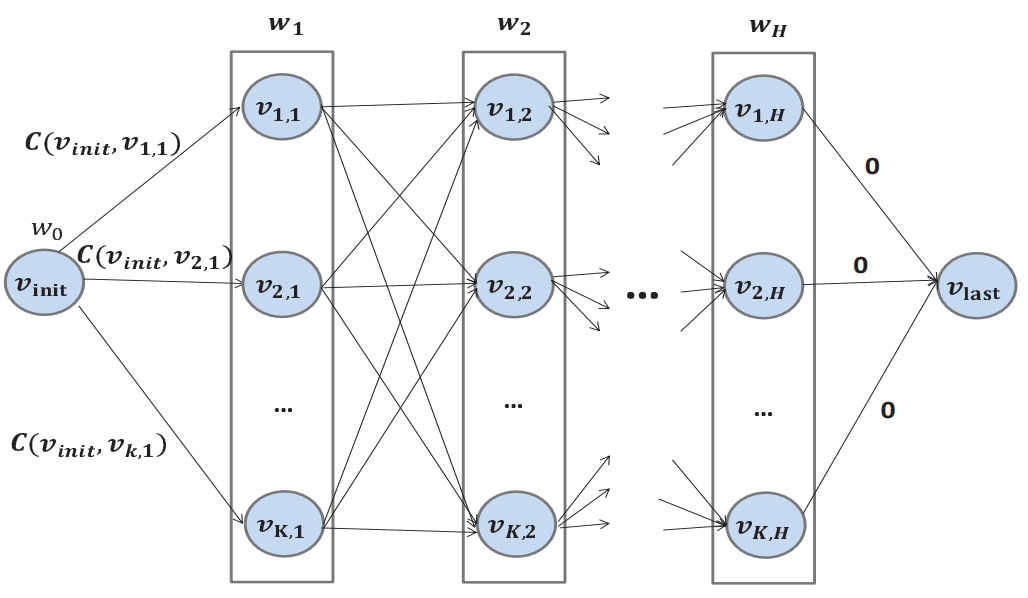
\includegraphics[scale=0.5]{ZacheilasGraph.PNG}
\caption{Graph der Zustandsübergänge \cite{zacheilas_elastic_2015}.}
\end{figure}

Um die optimalen Zustandsübergänge zu finden werden nun alle Kanten mit Gewichten versehen.
Die Gewichte der Kanten werden mit einer von Zacheilas et al. definierten Kostenfunktion bestimmt. Sie ist eine gewichtete Summe mit drei Summanden und wird durch folgenden Term definiert\cite{zacheilas_elastic_2015}:

\begin{equation*}
\begin{split}
C(v_{ij}v_{i^\prime j^\prime}) = VT_{i^\prime j^\prime} \times  C_A + p^\prime \times C_B + S(i,i^\prime) \times C_C \\
   S(i,i^\prime) =
   \begin{cases}
     0 & \text{wenn } i = i^\prime \\
     1 & \text{sonst} 
   \end{cases}
\end{split}
\end{equation*}


Der Erste der Summanden ist die Anzahl der verpassten Tupel im zukünftigen Zustand \(VT_{i^\prime j^\prime}\), die mit einem benutzerdefinierten Kostenfaktor \(C_A\) multipliziert werden.
Der zweite Summand erfasst die Kosten der Ressourcen, die benötigt werden um einen Operator auszuführen.
Die Kosten errechnen aus dem Produkt des zukünftigen Parallelisierungsgrades \(p^\prime\) und den benutzerdefinierten Kosten \(C_B\) eines einzelnen Tasks.
Der dritte Teil der Summe berücksichtigt den Aufwand, der durch skalieren eines Operators entsteht.
Das CEP-System muss hierzu die Verarbeitung der Tupel kurzfristig stoppen und das Routing in der Topologie anpassen.
Die Kostengewichtung \(C_C\) ist ebenfalls durch den Benutzer zu bestimmen.
Sind alle Kanten gewichtet kann anschließend mittels eines Algorithmus, der den kürzesten Pfad ermittelt, die optimale Abfolge von Zustandsübergängen berechnet werden.
Der erste Zustand in der gefundenen Abfolge bestimmt den Parallelisierungsgrad des Operators.

\section{Implementierung}

Im Folgenden sollen die Besonderheiten der Implementierung des Algorithmus für das Framework diskutiert werden.
Für die Implementation des Graphen der Zustandsübergänge wurde die Bibliothek JGraphT \cite{noauthor_welcome_nodate} verwendet.
Diese liefert ebenfalls eine Implementation des Dijkstra-Algorithmus um den kürzesten Pfad im Graphen zu bestimmen.
Die Umsetzung der Regression mittels Gauss-Prozessen erfolgte mit der Bibliothek Smile \cite{noauthor_smile_nodate}.

\subsection{Training des Vorhersagemodells}

Die Implementation verwendet ebenfalls das Graph-Modell des Frameworks.
Allerdings wird für die Vorhersage eine Historie der Messdaten aus dem CEP-System benötigt.
Da das Graph-Modell des Frameworks aber nur den aktuellen Status der Topologie repräsentiert, ist dieses nicht ausreichend.
Um das Modell für die Regression zu trainieren, werden deshalb CSV-Dateien eingelesen.
Das Regressions-Modell wird zu Beginn für alle Operatoren trainiert, sodass während des aktiven Betriebs nur noch das Graph-Modell verwendet wird.
Während dem Betrieb können die Regressions-Modelle der einzelnen Operatoren jeweils einzeln aktualisiert werden.
Ddie Laufzeit eines Training-Vorgangs beträgt \(O(n^3)\) \cite{zacheilas_elastic_2015}.
Aufgrund der Laufzeit ist es sinnvoll Operatoren während der Laufzeit einzeln aktualisieren zu können.
Bei der Aktualisierung des Modells eines Operators wird das alte Modell verworfen und durch ein neues ersetzt.
Das neue Modell wird ausschließlich aus den zuletzt eingelesenen Daten erzeugt.

Außerdem werden in der momentan implementierten Version des Algorithmus andere Eingabewerte als in der Originalversion verwendet.
Ursprünglich werden der momentane Zeitstempel, die Tageszeit und der Wochentag für die Vorhersage der eingehenden Tupel verwendet.
Um die ausgehenden Tupel vorherzusagen wird zusätzlich der Parallelisierungsgrad des Operators verwendet.
Da die Evaluation für Zeiträume in der Größenordnung weniger Stunden vorgesehen ist, ist die Verwendung dieser Werte nicht sinnvoll.
Die Tageszeit und der Wochentag wurden daher entfernt und durch die Zeit ersetzt, die seit Beginn der Evaluation vergangen ist.

\subsection{Vorhersage von verpassten Tupeln}

Ein essentieller Teil des Algorithmus ist die Kostenfunktion die auf der korrekten Vorhersage von verpassten Tupeln beruht.
Zacheilas et al. berechnen die Tupel wie folgt \cite{zacheilas_elastic_2015}:

\[\text{Verpasste Tupel} = \text{Anzahl eingehender Tupel} \times \text{Selektionsrate} - \text{Anzahl ausgegebener Tupel}\]

Die Selektionsrate stellt dabei das Verhältnis der Anzahl ausgegebener Tupel pro eingehendem Tupel dar.
Die Selektionsrate eines Operators wird als konstant angenommen.
Die Vorhersage von Verpassten Tupeln basiert daher auf der Vorhersage der Anzahl eingehender Tupel und der Anzahl ausgehender Tupel.
Ausgehende Tupel werden im von den Autoren vorgestellten System aber nicht gemessen.
Sie berechnen die Anzahl der ausgehenden Tupel basierend auf der vergangenen Zeit, dem Parallelisierungsgrad, der vorhergesagten Latenz des Operators und der Anzahl eingehender Tupel.
Da das in dieser Arbeit vorgestellte Framework die Daten für ausgehende Tupel liefert wird die Anzahl ausgehender Tupel für die Umsetzung des Algorithmus nicht berechnet.
Stattdessen werden anstatt der Latenz des Operators direkt die Anzahl ausgehender Tupel vorhergesagt.

\subsection{Kern der Gauss-Prozesse}
Für die Regression der Anzahl eingehender und ausgehender Tupel werden vom Algorithmus sogenannte Gauss-Prozesse verwendet.
Sie ermöglichen zu einem n-dimensionalen Eingabevektor \(x \in \mathbb{R}^n\) eine Schätzung des Zielwertes \(y\) zu berechnen.
Für diese Schätzung bedienen sich Gaußprozesse einer sogenannten Kovarianz-Matrix.
Die Kovarianz-Matrix wird mit einer Kovarianz-Funktion aus einem gegebenen Datensatz, den Trainingsdaten, berechnet.
Die Trainingsdaten bestehen aus mehreren n-dimensionalen Eingabevektoren \(x\) und deren zugehöriger Zielwert \(y\).
Die Kovarianz-Funktion \(k(x,x^\prime\) bestimmt die Korrelation zwischen zwei Eingabevektoren \(x \in \mathbb{R}^n\) aus den Trainingsdaten.
Die Wahl der Kovarianz-Funktion hat dabei maßgeblichen Einfluss auf die berechnete Korrelation der Werte und somit auch auf das Modell des Gauss-Prozesses.
Eine Kovarianz-Funktion muss per Definition symmetrisch sein \cite{rasmussen2004gaussian}.
Die Symmetrie der Kovarianz-Funktion bedeutet, dass \(k(x,x^\prime) = k(x,x^\prime)\) gilt.
Im Bereich des maschinellen Lernens wird die Kovarianz-Funktion auch Kern genannt.
Somit besitzt jeder Gauss-Prozess einen symmetrischen Kern, mit dessen Hilfe die Kovarianz-Matrix für die Vorhersage berechnet wird.

Zacheilas et al. verwenden für Ihre Vorhersagemodelle folgenden Kern:

\[k(x, x^\prime) = \sigma^2 \exp{\left( - \frac{1}{2} \sum^{n}_{d=1} \frac{x_d-x_{d}^{\prime}}{\lambda_d}\right)}\]

Wobei \(\sigma\) und \(\lambda\) hyperparameter des Modells darstellen.
Sie werden im Kapitel ******************** Parameter betrachtet.
Es ist offensichtlich erkennbar, dass der von den Autoren vorgeschlagene Kernel nicht symmetrisch ist.
Das Ergebnis der Subtraktion von \(x_d - x^\prime_d\) kann sowohl positiv als auch negativ sein.
Somit ist der Kern keine gültige Kovarianz-Funktion.
Für die vorliegende Implementation wurde der Kern wie folgt geändert, sodass der Ergebnis der Subtraktion als absoluter Betrag verwendet wird.


\[k(x, x^\prime) = \sigma^2 \exp{\left( - \frac{1}{2} \sum^{n}_{d=1} \frac{|x_d-x_{d}^{\prime}|}{\lambda_d}\right)}\]

Grundsätzlich ist der Kern in Smile als Java-Interface implementiert und somit durch jede beliebige Kovarianz-Funktion austauschbar.

\subsection{Pfad-Zurückweisung}

Zacheilas et al. sehen in der Originalversion des Algorithmus eine Zurückweisung eines gefundenen kürzesten Pfades vor.
Die durch die Verwendung des Gauss-Prozesses vorhergesagten Werte unterliegen einer Normalverteilung.
Mit Hilfe der Standardabweichung der Normalverteilung kann berechnet werden, wie wahrscheinliches es ist, dass der vorhergesagte Mittelwert eintrifft \cite{zacheilas_elastic_2015}.
Diesen Umstand nutzen die Autoren um einen gefundenen Pfad zurückzuweisen, falls der Eintritt des vorhergesagten Wertes zu unwahrscheinlich ist.
Diese Funktionalität ist in der momentanen Version der vorliegenden Implementation im Framework nicht vorhanden.

\section{Parameter}

Dieser Abschnitt beschreibt die Parameter die es ermöglichen den Algorithmus anzupassen.
In dem Fall des Regression-Algorithmus dienen Sie hauptsächlich dazu das unterliegende Kosten- und Regressionsmodell anzupassen.
Wie bei dem Algorithmus mit Warteschlangentheorie werden die im Graph-Modell festgelegten minimalen und maximalen Parallelisierungsgrade berücksichtigt.
Die folgenden Parameter sind als finale statische Attribute in den Klassen der Implementation des Algorithmus zu finden.

\subsection{Trainingsdaten}

Name: INPUT\_TRAINING\_DATA\_FOLDER / OUTPUT\_TRAINING\_DATA\_FOLDER

Standardwert: null

Wertebereich: alphanumerisch

Gibt den Pfad zu dem Ordner mit den Dateien an, die die Trainingsdaten für die Regressionsmodelle beinhalten.
Die Daten müssen im CSV-Format bereitgestellt werden.
Dabei ist zu beachten, dass als Trennzeichen das Leerzeichen erwartet wird.
Für jedes Vorhersagemodell wird eine eigene Datei mit Daten benötigt.
Es wird somit erwartet, dass in dem angegebenen Verzeichnis zwei Dateien pro Operator vorliegen.
Eine Datei beinhaltet die Daten für die Vorhersage der Anzahl eingehender Tupel.
Die Andere stellt die Daten für die Vorhersage der Anzahl ausgehender Tupel bereit.
Die Datei für eingehende Tupel muss folgenden Namen besitzen: ''<Operator>\_input\_train.csv''.
Analog gilt für ausgehende Tupel ''<Operator>\_output\_train.csv''.

Die Trainingsdaten für eingehende Tupel bestehen momentan aus drei Spalten.
Als Daten für den Eingabevektor: Unix-Zeitstempel in Sekunden, Sekunden seit Start der Anwendung.
In der letzten Spalte wird die Zielvariable Anzahl eingegangener Tupel erwartet.
Die Trainingsdaten für ausgehende Tupel umfassen vier Spalten.
Eingabevektor: Unix-Zeitstempel, Sekunden seit Start der Anwendung, Parallelisierungsgrad.
Wieder in der letzten Spalte muss die Anzahl ausgehender Tupel stehen.
Die Anzahl der Spalten für eingehende und ausgehende Tupel wird über einen Enumerator gesteuert.
Dieser muss angepasst werden, falls sich die Spaltenanzahl ändert.
Ebenso muss die Dimension von \(\lambda\) mit der Dimension der Eingabewerte übereinstimmen.

\subsection{Hyperparameter}

\begin{table}[!htbp]
\centering
\caption{Hyperparamter}
\begin{tabular}{l|r|r}
\hline
\textbf{Name} & \textbf{Standardwert} & \textbf{Wertebereich} \\
SIGMA\_INPUT & 1.0 & \(x \in \mathbb{R} > 0 \) \\
LAMBDA\_INPUT & (1.0, 1.0) &  \(x \in \mathbb{R}^2 > 0 \) \\
SIGMA\_OUTPUT & 1.0 & \(x \in \mathbb{R} 0 \) \\
LAMBDA\_OUTPUT & (1.0, 1.0, 1.0) & \(x \in \mathbb{R}^3 0\) \\
\hline
\end{tabular}
\end{table}

Die Hyperparameter dienen hauptsächlich der Konfiguration des Kernels.
Sigma ist eine Größe mit der der Kernel multipliziert wird.
Der Parameter kann dazu verwendet werden die Korrelation der Werte grundsätzlich zu verkleinern oder zu vergrößern.
Lamda wird verwendet um die Komponenten des Eingabevektors zu gewichten.
Für den verwendeten Kernel bedeutet das, dass der negative Exponent kleiner wird wenn \(lambda\) größer wird.
Im Umkehrschluss fällt die Korrelation für diesen Wert des Eingabevektors höher aus.

Der Wert für den Zeitstempel verdient besondere Beachtung.
Da der Zeitstempel einen absoluten Zeitpunkt markiert, verändert sich die Korrelation mit jeder Anwendung des Kernels.
Hier muss das \(lambda\) gegebenenfalls nachjustiert werden.
Das \(lambda\) für die Vorhersage der ausgehenden Tupel sollte zusätzlich berücksichtigen, dass der Parallelisierungsgrad im Normalfall eine kleinere Größenordnung als die anderen Werte besitzt.
Daher weist der Parallelisierungsgrad tendenziell höhere Korrelationen auf als die anderen Komponenten.
Dieser Umstand sollte gegebenenfalls mit \(lambda\) ausgeglichen werden.

\subsection{Kostenfunktion}

Die vorgestellte Kostenfunktion bietet drei verschiedene Eingabegrößen, die durch den Benutzer getätigt werden müssen.
Die Kostenfunktion implementiert ein Interface und wird bei der Erzeugung der Regressionsmodelle als Parameter übergeben
Somit ist die Kostenfunktion gegen andere Varianten austauschbar.
Die Kostenfaktoren der Funktion können über den Konstruktor angegeben werden.
Bei einem parameterlosen Aufruf des Konstruktors initialisiert dieser die Funktion mit eins.





\chapter{Evaluation}

Im diesem letzten Teil der Arbeit sollen die beiden Implementierungen der Algorithmen evaluiert und miteinander verglichen werden.
Für die Evaluation sollen die Algorithmen das CEP-System Heron über das implementierte Framework kontrollieren, während ein möglichst realitätsnaher Strom von Tupeln vom System abgearbeitet werden muss.

Das folgende Kapitel gliedert sich in mehrere Teilbereiche.
Zuerst müssen Daten erhoben werden, die während der Evaluation vom System verarbeitet werden müssen.
Hierzu wurden Tweets von der Twitter-Streaming API ausgelesen und gesichert.
Diese reflektieren realitätsnahe Schwankungen des Arbeitsaufwandes.
Anschließend wird der Systemaufbau für die Evaluation durchgeführt.
Außerdem wird kurz die Wahl von Heron als System für die Evaluation und dessen spezielle Eigenschaften erläutert.
Für die Evaluation ist zudem eine Topologie notwendig.
Diese definiert wie die im ersten Schritt erhobenen Daten während der Evaluation verarbeitet werden.
Dazu wurde speziell für die Evaluation eine neue Topologie entwickelt, die Tweets einliest und anschließend analysiert.
Im darauf folgenden Teil werden die in den vorherigen Kapiteln beschriebenen Parameter der Algorithmen für die Evaluation definiert und deren Wahl begründet.
Anschließend wird noch ein kurzer Überblick über den Ablauf der Evaluation gegeben.

Zum Ende des Kapitels wird die Evaluation der Algorithmen mit den erhaltenen Messwerten  durchgeführt.
Das Ziel ist dabei, dass die Algorithmen auf Basis der Parallelisierungsgrade, der Tupel-Latenz und der Fehlerrate von Tupeln miteinander verglichen werden.
So kann der Schluss gezogen werden, welcher Algorithmus die Topologie während der Analyse der vorliegenden Daten besser gesteuert hat.


\section{Testdaten}
Um einen realitätsnahen Datenstrom erzeugen zu können, wurden während dem August 2018 Tweets von der Twitter-Streaming API abgerufen und gespeichert.
Neben kostenpflichtigen Schnittstellen bietet die API kostenlos einen kontinuierlichen Datenstrom von zufällig gewählten Tweets.
Die gewählten Tweets sind dabei für jeden Konsumenten, der sich für den Datenstrom registriert hat, identisch \cite{noauthor_get_nodate}.
Der Datenstrom liefert ca. 1\% der gesamten anfallenden Twitter-Daten in Realzeit \cite{noauthor_how_2017}.
Dies sind neben neuen Statusupdates (Tweets) auch Löschanfragen zu bestehenden Tweets.
Aus Gründen der besseren Lesbarkeit werden im Folgenden beide Arten der Statusänderung als Tupel bezeichnet.
Für die Evaluation werden die gesammelten Tupel der Woche vom 7. - 13. August 2018 verwendet.

In dieser Zeit wurden 32.416.487 Tupel erfasst die ca. 160 GB Textdaten entsprechen.
Die Abbildung 9.1 zeigt die Verteilung der Anzahl erfasster Tupel pro Stunde im Verlauf der Woche.
Beginn der Aufzeichnung ist Dienstag, 07.08.2018 00:00 UTC.


\begin{figure}
 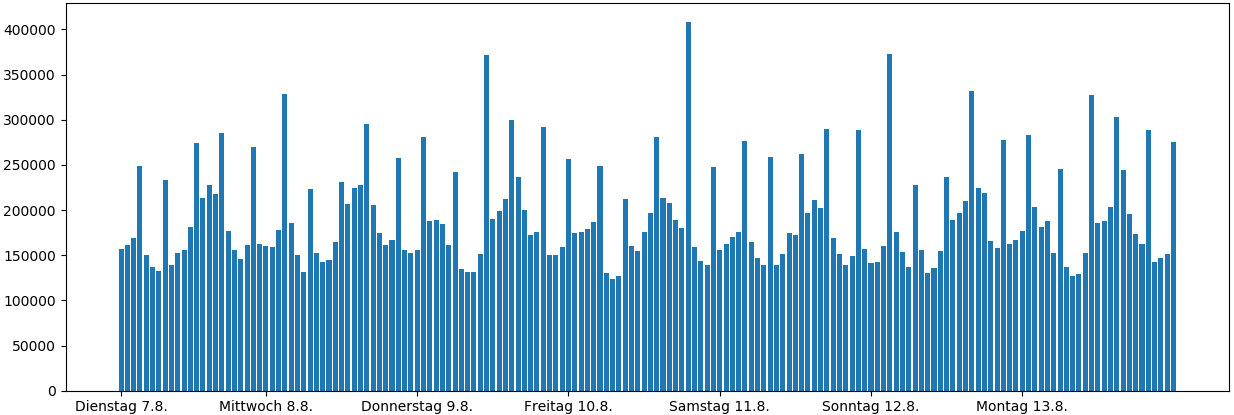
\includegraphics[scale=0.45]{Twitter-Daten.png}
 \caption{Anzahl Tupel pro Stunde.}
\end{figure}

\section{Systemaufbau}
Die Evaluation wurde auf dem internen OpenStack-Cluster des Instituts für Verteile und Parallele Systeme der Universität Stuttgart durchgeführt.
Für die Evaluation wurde ein Cluster aus vier virtuellen Maschinen aufgebaut.
Die Maschinen werden mit dem Betriebssystem Ubuntu 14.04 betrieben.
Drei der virtuellen Maschinen sind je mit 24 CPU-Kernen, 32 GB Arbeitsspeicher und 50 GB persistentem Speicher ausgestattet.
Diese Maschinen führen während der Evaluation die aktiven Tasks aus.
Die vierte Maschine wird als Steuer-Knoten genutzt und arbeitet mit 4 CPU-Kernen, 8 GB RAM sowie 10 GB persistentem Speicher.
Auf der vierten Maschine wird ausschließlich der Ablauf der Evaluation gesteuert.
Somit sind alle Maschinen, die Tasks der Topologie ausführen, identisch.

Der Cluster wird über den Apache Aurora-Scheduler in der Version 0.13 gesteuert.
Der Scheduler von Aurora sowie die Steuerung von Heron befinden sich auf dem Steuer-Knoten.
Der Adapter für das implementierte Framework wird ebenfalls auf diesem Rechner gestartet.
Auf jedem der drei anderen Rechner ist die ausführende Instanz von Aurora ebenfalls in der Version 0.13 installiert.
Um die Arbeitspakete an die ausführenden Rechner auszuliefern, wird das verteile Dateisystem HDFS von Apache Hadoop in der Version 3.0.3 verwendet.
Zusätzlich benötigen die Systeme Apache Zookeeper um den verteilten Zustand zu speichern.
Dieser ist als Cluster über alle vier virtuellen Maschinen konfiguriert.

\section{Heron}
Für die Evaluation wurde das CEP-System Heron gewählt \cite{kulkarni_twitter_2015}.
Heron ist ein Nachfolger von Apache Storm.
Die Twitter Inc. entwickelte Heron als Nachfolger für den produktiv verwendeten Storm Cluster.
Sie entwickelten Heron als schnelleres und besser skalierendes System, da Storm den Anforderungen nicht mehr gerecht werden konnte \cite{kulkarni_twitter_2015}.
Heron wird von Twitter momentan als produktives System für die Analyse von Datenströmen eingesetzt.
Heron wurde für diese Evaluation aus zwei Gründen gewählt.
Einerseits ist aufgrund der produktiven Verwendung und aktiven Entwicklung bei Twitter ist davon auszugehen, dass das System aktuellen, realen Anforderungen gerecht wird.

Zweitens wurde ein System gesucht, mit dem die Algorithmen möglichst unabhängig bewertet werden können.
Viele der in Kapitel drei vorgestellten Algorithmen wurden auf Basis eines bestimmten CEP-Systems oder einem anderen Datenstrom verarbeitenden System entwickelt.
Einige dieser Systeme sind Eigenentwicklungen oder erweiterte Frameworks auf bestehenden Systemen, die von den Autoren entwickelt werden.
Apache Storm wird ebenso, als eines der bekanntesten, oft als Basis für die Entwicklung von neuen Algorithmen verwendet.
Mit Heron können verschiedene Algorithmen getestet werden, ohne dass manche den Vorteil besitzen nativ für das CEP-System entwickelt worden zu sein.

Eine wichtige Neuerung bei Heron ist besonders hervorzuheben:
Das System bietet die Möglichkeit eine Topologie über eine autonome Strom-Regulierung zu steuern \cite{kulkarni_twitter_2015}.
Bei vielen anderen Systemen werden Tupel einfach verworfen, wenn die Kapazität eines Operators nicht mehr ausreicht.
Dieses Verhalten wird als sogenannter Lastabwurf bezeichnet.
Dies führt dazu, dass Tupel entweder verloren gehen oder von der Quelle erneut ausgegeben werden.
Wird ein Tupel neu ausgegeben, muss es alle Operatoren erneut durchqueren.
Dieses Verhalten erzeugt zusätzliche Last auf dem System und verstärkt den Engpass.
Die neue Regulierung in Heron wird aktiviert, wenn ein Operator die ankommende Menge von Tupel nicht mehr verarbeiten kann.
Dies wird von der Topologie erkannt und die Quellen werden daraufhin gestoppt.
Somit gelangen keine neuen Tupel mehr in die Topologie.
Die Regulierung stoppt die Quellen so lange, bis der Operator wieder genügend Kapazität für neue Tupel geschaffen hat.

Diese Methode, den Datenstrom zu drosseln, verändert die Erkennung von Operatoren, die Flaschenhälse bilden, gänzlich.
Messwerte, auf die viele der in Kapitel drei vorgestellten Algorithmen reagieren, verhalten sich anders.
Dies trifft auch für die beiden implementierten Algorithmen zu.
Diese gehen im Grundprinzip davon aus, dass bei einem Flaschenhals die Anzahl ankommender Tupel größer als die Anzahl abgearbeiteter Tupel ist.
Dieser Zustand kann aber nicht mehr auftreten, wenn die Quelle den Zufluss von neuen Tupeln automatisch stoppt.
Somit würde ein Operator gar nicht oder nur sehr schwach von den Algorithmen skaliert werden.
Deswegen wurde dieses Verhalten für die Evaluation der beiden Implementierungen deaktiviert.

Die Evaluation wurde mit Heron unter der aktuellen Version 0.17.5 durchgeführt.
Die System-Parameter wurden im Standard belassen und nicht verändert.

\section{Topologie}

Für die Durchführung der Evaluation wurde eine eigene Topologie entwickelt.
Diese liest die von der Twitter API gesammelten Tupel aus und analysiert sie auf deren Eigenschaften.
Der logische Aufbau der Topologie ist in der Abbildung 10.2 dargestellt.
Ziel bei der Erstellung der Topologie war, dass es Operatoren mit unterschiedlich großen Lasten gibt.
Entweder wurde der Datenstrom durch eine Filteroperation für den Folgeoperator verkleinert oder die Funktion des Operators rechenintensiv gestaltet.

\begin{figure}
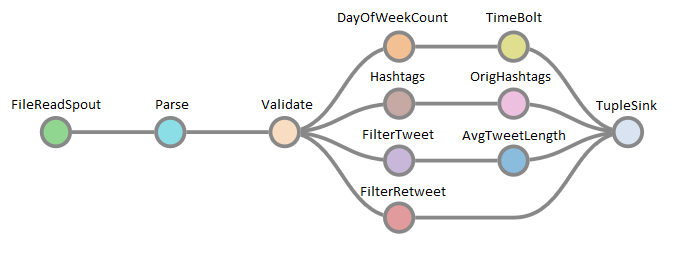
\includegraphics[scale=0.8]{Topologie.png}
\caption{Darstellung der logischen Topologie durch Heron UI.}
\end{figure}

Topologien in Heron besitzen Parameter, durch die der Entwickler deren Verhalten beeinflussen kann.
Für nahezu alle Parameter definiert Heron einen Standardwert.
Im Folgenden werden die Parameter beschrieben, bei der die Evaluations-Topologie vom Standard abweicht.
Die Parameter sind in Tabelle 10.1 mit den zugewiesenen Werten aufgelistet.

Wie schon im vorherigen Kapitel beschrieben wurde die Regulation des Tupel-Stroms deaktiviert.
Die Topologie wurde so konfiguriert, dass jedes Tupel mindestens einmal erfolgreich verarbeitet werden muss.
Deshalb werden Tupel, die in der Folge eines Flaschenhalses verworfen werden, mehrfach von der Quelle ausgegeben.
Dies ist möglich, weil die Bestätigung von Tupel aktiviert wurde.
Dies bedeutet, dass jeder Operator die Bearbeitung des Tupels an die Quelle zurückmeldet.
Erst wenn alle Operatoren die Verarbeitung des Tupel bestätigen, wird das Tupel als bestätigt markiert.
Durch diesen Mechanismus ist es ebenfalls möglich die Latenz des Tupels zu bestimmen.

Die Quelle wurde so konfiguriert, dass ein Tupel, das innerhalb von einer Minute nicht erfolgreich verarbeitet wurde, ungültig ist und wiederholt werden muss.
Außerdem sendet die Quelle maximal 1.000.000 Tupel, ohne dass eines davon bestätigt wurde.
Das bedeutet, dass sich zu jedem Zeitpunkt maximal 1.000.000 Tupel zur Bearbeitung in der Topologie befinden.
Dieser Wert wurde bewusst sehr groß gewählt, um die Ausgabe von Tupeln nicht aufgrund von Flaschenhälsen in der Topologie zu verringern.
So ist sichergestellt, dass die Quelle dauerhaft in der Lage ist Tupel auszugeben, um den realistischen Arbeitsaufwand zu rekonstruieren.

\begin{table}
\caption{Parameter der Topologie}
\begin{tabular}{ll}
\hline
\textbf{Parameter} & \textbf{Wert} \\ \hline
TopologyDropTuplesUponBackpressure & True \\
TopologyReliabilityMode & ATLEAST\_ONCE \\
MessageTimeoutSecs & 60 \\
MaxSpoutPending & 1000000 \\
\hline
\end{tabular}
\end{table}

In der momentanen Version kann Heron die Operatoren nur skalieren, wenn die Tupel zufällig den Tasks der Operatoren zugewiesen werden.
Deswegen wurde diese Konfiguration für die Operatoren der Topologie gewählt.
Außerdem erhält jeder Folgeoperator immer alle ausgegebenen Tupel des Vorgängers.
Es gibt also keine selektive Weiterleitung.
Jedem Task wurde ein CPU-Kern, 1,25 GB RAM und 1,25 GB persistentem Speicher zugewiesen.
Die Topologie wurde mit der Java API von Heron entwickelt.
Diese erlaubt das definieren eigener Logik für die Quelle und die anderen Operatoren.
Im Folgenden werden die einzelnen Operatoren der Topologie beschrieben.

\subsection{Quelle}
Die Quelle ''FileReadSpout'' liest die gesammelten Daten von der Festplatte.
Dies geschieht Zeile für Zeile, was jeweils einem Tupel entspricht.
Jedes erfasste Tupel besitzt einen Zeitstempel mit dem Zeitpunkt, an dem es erzeugt wurde.
Um den Twitter-Datenstrom realistisch nachzubilden wird dabei immer der Zeitstempel des eingelesenen Tupels überprüft.

Um die Topologie auszulasten ist der Datenstrom in der realen Geschwindigkeit, mit der er erfasst wurde, jedoch nicht ausreichend.
Deshalb wird der Zeitraum, in dem die Tupel erfasst wurden, auf einen kleineren Zeitraum komprimiert.
So bleibt die Struktur des Arbeitsaufwandes wie Lastspitzen und Lastabfall erhalten, wird aber in ein kürzeres Intervall geschoben um so insgesamt mehr Last zu erzeugen.
Das Ziel ist, dass in jeder realen Minute in der Evaluation 84 Minuten der aufgezeichneten Daten verarbeitet werden.
Somit werden in einer realen Stunde 84 Stunden der aufgezeichneten Daten abgearbeitet.
Da eine Woche 168 Stunden hat dauert ein Durchlauf der Evaluation 2 Stunden.
Durch die Kompression der Daten, kann ein Arbeitsaufwand erzeugt werden, der die Operatoren so auslastet, dass sie skaliert werden müssen.

Die Quelle wurde so implementiert, dass sie die Tupel anhand des Zeitstempels mit realistischen Schwankungen abgibt.
Dazu speichert sie den Startzeitpunkt der Topologie sowie den Zeitstempel des ersten Tupels in Millisekunden.
Während der Evaluation wird geprüft wie viele Millisekunden seit dem Start der Topologie vergangen sind.
Mit diesen Werten kann der maximale Zeitstempel errechnet werden, mit dem ein Tupel die Quelle verlassen darf.
Der maximale Zeitstempel errechnet sich aus der Differenz von aktuellem Zeitstempel und der Startzeit der Topologie, die mit dem Faktor 84 multipliziert und zu dem Zeitstempel des ersten Tupels addiert wird.
Mit dieser Methode kann nicht garantiert werden, dass Tupel nicht langsamer ausgegeben werden.
Aber es wird verhindert, dass die Tupel schneller als der realistische Arbeitsaufwand ausgeben werden.

Die Leserate vom permanenten Speicher ist in der verwendeten Implementierung wesentlich höher als die Rate des komprimierten Arbeitsaufwandes, sodass eine langsamere Abgabe der Tupel unrealistisch ist.

\subsection{Andere Operatoren}

Um die folgenden Funktionen zu verstehen, sind erst folgende Erläuterungen notwendig.
Ein Retweet ist ein Statusupdate das das Statusupdate eines anderen Nutzers ohne weitere Anmerkung weiterverbreitet \cite{noauthor_docs_nodate}.
Ein Antwort-Tweet ist ein Statusupdate, das auf das Statusupdate eines anderen Nutzers antwortet \cite{noauthor_docs_nodate}.
Ein Tweet zitiert einen anderen Tweet wenn er ihn weiterverbreitet und Anmerkungen hinzufügt \cite{noauthor_docs_nodate}.

Außerdem ist zu bemerken, dass alle Operatoren Tupel direkt weiterverarbeiten und keine Fenster bilden.
Dies liegt daran, dass Heron keine Bearbeitungsdauer der Tupel misst.
Somit können die Modelle der Warteschlangen-Theorie für Operatoren mit Fenstern nicht angewendet werden.

\begin{itemize}
\item{''Parse'': Dieser Operator erhält das von der Quelle ausgegebene Tupel. Dieses enthält einen String, der ein JSON-Objekt beschreibt. Die Daten des JSON-Objektes werden ausgelesen und als getrennte Attribute in einem Tupel weitergeleitet. Löschanfragen für Statusmeldungen werden nicht weitergeleitet.}
\item{''Validate'': Dieser Operator prüft die Lesbarkeit der Daten und gibt sie auf der Standardausgabe aus.}
\item{''DayOfWeekCount'': Hier wird der Zeitstempel des Tupels in den Wochentag, an dem das Tupel erzeugt wurde, umgerechnet. Jedes Tupel erhöht den Zähler für den jeweiligen Tag.}
\item{''TimeBolt'': Dieser Operator gibt den genauen Datumstext für den Zeitstempel des Tupels auf der Standardausgabe aus.}
\item{''Hashtags'': Hier werden die Hashtags des Tweets ausgelesen. In einer Tabelle werden identische Hashtags gezählt.}
\item{''OrigHashtags'': Zählt ebenso Hashtags, allerdings nur für Original-Tweets eines Retweet oder Antwort-Tweet.}
\item{''FilterTweet'': Sendet nur Tweets weiter, die kein Retweet und kein Antwort-Tweet sind sowie keinen anderen Tweet zitieren.}
\item{''AvgTweetLength'': Berechnet die durchschnittliche Länge des verfassten Textes.}
\item{''FilterRetweet'': Sendet ausschließlich Retweets weiter.}
\item{''TupleSink'': Hat keine Operation außer die Tupel final zu bestätigen.}
\end{itemize}

\section{Ablauf}

Für die Evaluation müssen die in dieser Arbeit implementierten Algorithmen die beschriebene Topologie steuern, während sie die Tupel im Zeitfenster von zwei Stunden verarbeitet.
Alle Operatoren starten dabei mit einem Parallelisierungsgrad von eins.
Für jeden der beiden Algorithmen von Lohrmann et al. und Zacheilas et al. wurden fünf Durchläufe gestartet.
Jeder Durchlauf startet, wenn die Topologie aktiviert wird.

Die Hauptsteuerung wurde so implementiert, dass sie alle fünf Minuten die Topologie durch den gewählten Algorithmus prüfen lässt.
Zuerst werden alle Messwerte des Graphen-Modells mit den aktuellen Messwerten aus der Topologie aktualisiert.
Anschließend wurden die folgenden Daten zur Evaluation erfasst:
\begin{itemize}
\item{Minuten seit Beginn der Evaluation}
\item{Sekunden seit Beginn der Evaluation}
\item{Durchschnittliche Latenz der Tupel}
\item{Anzahl fehlgeschlagener Tupel}
\item{Anzahl bestätigter Tupel}
\item{Summe der Parallelisierungsgrade der Operatoren}
\end{itemize}
Der erste Start der Hauptsteuerung erfolgt zur ersten Prüfung, nachdem die Topologie schon 5 Minuten aktiv ist.
Deshalb ist die Anzahl der Minuten und Sekunden seit Beginn der Evaluation um fünf Minuten verschoben.
Wenn alle Messwerte erfasst sind, startet der gewählte Algorithmus und die Topologie wird entsprechend der Empfehlung des Algorithmus skaliert.
Erst nachdem der Vorgang erfolgreich von Heron zurückmeldet wurde, beginnt das Zeitfenster von 5 Minuten bis zur nächsten Prüfung.

Während Heron die Topologie skaliert ist diese gestoppt, sodass während dieser Zeit keine neuen Tupel von der Quelle ausgegeben werden.
Das wirkt sich offensichtlich auf die Zeitbeschränkung für die Tupel-Ausgabe der Quelle aus: 
Die Zeit, die seit Beginn der Evaluation vergangen ist, läuft trotzdem weiter.
Dies spiegelt auch das reale Verhalten wieder, da der reale Datenstrom ebenfalls zwischengespeichert werden müsste, solange die Topologie skaliert.

Während des Vorgangs löscht Heron außerdem alle Messdaten, da die alten Daten für den aktuellen Zustand der Topologie nicht mehr gültig sind.
Nachdem die Topologie wieder gestartet wurde, müssen sich die Zwischenspeicher vor und nach den Operatoren erst wieder mit Tupel füllen, um aussagekräftige Messwerte zu erhalten.
Deswegen ist es sinnvoll erst nachdem die Topologie skaliert wurde weitere fünf Minuten zu warten, damit die Messwerte im System wieder aussagekräftig sind.

Außerdem werden aus diesem Grund bei der Abfrage der Messwerte, die ebenfalls im Intervall von fünf Minuten ausgelesen werden, nur die letzten drei Minuten aus dem CEP-System angefordert.
Dies bedeutet, dass die Messwerte der ersten zwei Minuten, nachdem die Topologie skaliert wurde, weder für die Berechnung des Parallelisierungsgrades noch für die Ergebnisse der Evaluation verwendet wurden.

Die Evaluation stoppt sobald alle Tupel verarbeitet wurden.

\section{Parametrisierung der Algorithmen}

Für die Durchführung der Evaluation mussten die beschriebenen Parameter der Algorithmen definiert werden.
Das Graphen-Modell war so konfiguriert, dass der minimale Parallelisierungsgrad eins und der maximale zehn beträgt.
Die maximale Latenz des Pfades wurde auf 10 ms gesetzt.
Da jeder Task eines Operators eine CPU, und 1,25 RAM verbraucht, konnte aufgrund der verfügbaren Ressourcen der maximale Parallelisierungsgrad nicht höher als zehn gesetzt werden.

Für die Evaluation wurden für den Warteschlangen-Algorithmus die in der Tabelle 10.3 gelisteten Parameter gewählt.
Wie im Original von Lohrmann et al. wurde die Erkennung eines Flaschenhalses ab einer Auslastung von 100\% gesetzt.
Der Koeffizient für adaptives Batching wurde auf null gesetzt, da Heron diese Methode nicht verwendet.
Der Parameter bestimmt ohnehin nur den Anteil der maximalen Latenz des Pfades, der für adaptives Batching reserviert ist.
So kann dieser Anteil auch direkt bei der Angabe der maximalen Latenz berücksichtigt werden, wenn der Parameter auf null steht.
Die Schrittweite des Algorithmus wurde ebenfalls wie im Original auf eins gesetzt.
Die Verwendung des Koeffizienten e wurde deaktiviert, da die gemessene Latenz im Vergleich zu der vom Algorithmus berechneten Latenz sehr hoch war.
Dies hätte wie in Kapitel 7.2.4 beschrieben dazu geführt, dass der Algorithmus sehr hohe Parallelisierungsgrade vorgeschlagen hätte.
Dies hätte in Kombination mit dem maximalen Parallelisierungsgrad von zehn zur Folge gehabt, dass die Topologie während der Evaluation konstant maximal skaliert ist und nie angepasst wird.

\begin{table}
\caption{Parameter für den Warteschlangenalgorithmus}
\centering
\begin{tabular}{ll}
\hline
\textbf{Parameter} & \textbf{Wert} \\ \hline
BOTTLENECK\_THRESHOLD & 1.0 \\
ADAPTIVE\_BATCHING\_COEFFICIENT & 0.0 \\
DELTA\_STEP\_SIZE & 1 \\
USE\_LATENCY\_ADAPTION & False\\
\hline
\end{tabular}
\end{table}

Für den zweiten Algorithmus wurden die in Tabelle 10.4 gezeigte Parametrisierung gewählt.

Die Trainingdaten für den Algorithmus wurden während der Evaluation des Algorithmus von Lohrmann et al. gesammelt.
Alle fünf Minuten, in denen die neuen Metriken aus dem System abgerufen wurden, wurden für jeden Operator die Anzahl eingegangener und ausgegangener Tupel der letzten drei Minuten mit Zeitstempel versehen und gespeichert.
Da die aus der Topologie bezogenen Messdaten vom aktuellen Zustand der Topologie und nicht von den verwendeten Twitter-Daten abhängen, sind auch Fehler reflektiert, die vom Algorithmus von Lohrmann et al. gemacht werden.
Somit ist garantiert, dass die verwendeten Trainingsdaten das Vorhersage-Modell nicht speziell für den vorliegenden Twitter-Datensatz übertrainieren.

Die Hyperparameter wurden für die Evaluation nicht mathematisch optimiert.
Sie wurden lediglich so gewählt, dass die Regression Vorhersagen im richtigen Größenbereich trifft.
Dazu wurden die Zeitstempel sehr schwach gewichtet.
Die Zeit, die seit der Evaluation vergangen ist, wurde stark gewichtet, da sie einen größeren Zusammenhang mit dem Zustand der Topolgie aufweist als der Zeitstempel.
Das Modell für eingehende Tupel beruht nur auf den beiden Dimensionen Zeitstempel und vergangene Zeit.
Daher muss die vergangene Zeit stark gewichtet werden um zu verhindern, dass der Zeitstempel das Modell verfälscht.

Für die Vorhersage der ausgehenden Tupel wurde die Gewichtung des Parallelisierungsgrad so gewählt, dass er sich in etwa gleich wie die vergangene Zeit auf die Korrelation auswirkt.
Wie in Kapitel 8.2.2 erwähnt besitzen der Parallelisierungsgrad und die Zeit, die seit der Evaluation vergangen ist, verschiedene Größenordnungen.
In der Evaluation bewegen sich Parallelisierungsgrade im Einerbereich währen die Zeit bis zu 7200 steigt.
Dies wird durch den gewählten Wert des Hyperparameters ausgeglichen.

Die Kostenfunktion wurde für alle Kostenfaktoren mit eins initialisiert.
Dies fördert die Flexibilität der Topologie, da die Kosten, die Topologie zu ändern, und die Kosten pro verwendeten Task sehr gering sind.
Die Anzahl verpasster Tupel kann jedoch schnell 1000 übersteigen, sodass die Kosten für verpasste Tupel ausschlaggebend für den kürzesten Pfad im Graphen der Zustandsübergänge sind.

Die Vorhersagen wurden für Zeitfenster von fünf Minuten getroffen, um gleich dem Intervall zu sein, in dem die Topologie geprüft wird.
Es wurden jede Runde Vorhersagen für sechs Zeitfenster getroffen, sodass immer Zustandsübergänge für die nächsten 30 Minuten berücksichtigt wurden.

\begin{table}
\caption{Parameter für den Algorithmus mit Regression} 
\centering
\begin{tabular}{ll}
\hline
\textbf{Parameter} & \textbf{Wert} \\ \hline
SIGMA\_INPUT & 1.0 \\
LAMBDA\_INPUT & (1.0, 10000.0) \\
SIGMA\_OUTPUT & 1.0 \\
LAMBDA\_OUTPUT & (1.0, 10000.0 10.0) \\
Kostenfunktion & (1.0, 1.0, 1.0) \\
Abstand Zeitfenster & 300 \\
Anzahl Zeitfenster & 6 \\
\hline
\end{tabular}
\end{table}

\section{Ergebnisse}

Im Folgenden werden für die Beurteilung der beiden Algorithmen die Messwerte verwendet, die während der Evaluation erfasst wurden.
Diese reflektieren kein festes Intervall von fünf Minuten, da die Wartezeit von fünf Minuten jeweils erst nach der Bestätigung, dass erfolgreich skaliert wurde, beginnt.
Außerdem ist zu beachten, dass die gezeigten Auswertungen jeweils zur Minute fünf der Evaluation beginnen, da zu Beginn der Evaluation offensichtlich keine Messwerte vorliegen.
Die folgenden Abkürzungen werden für die Algorithmen verwendet um die Lesbarkeit zu verbessern:
Algorithmus mit Warteschlangen Theorie (WT), Algorithmus mit Regression (RG).

\subsection{Parallelisierungsgrad der Topologie}
Um alle weiteren Messwerte zu verstehen ist es essentiell, dass der Zustand, in dem die Topologie während des Mess-Zeitraums befand, betrachtet wird.
Deshalb wurde jeweils der summierte Parallelisierungsgrad der Topologie gemessen.
Wie in Abbildung 9.3 zu sehen ist, verlaufen die Parallelisierungsgrade unter den beiden Algorithmen sehr unterschiedlich.

Zu Beginn skalieren beide Algorithmen die Topologie nach oben. Es ist ersichtlich, dass WT den Parallelisierungsgrad der Operatoren schrittweise verdoppelt, während RG etwas schneller ansteigt.

Nach dem initialen Anstieg schwankt der Parallelisierungsgrad unter WT sehr stark.
WT nimmt über die Evaluation hinweg viele Anpassungen vor und tendiert dazu, stark zwischen hohen und niederen Werten zu schwanken, da er nur reaktiv auf die letzten drei Minuten reagiert.
Bei hohem Parallelisierungsgrad geht dabei die Latenz der Tupel stark zurück, sodass der Algorithmus ihn verringert.
Ist der Parallelisierungsgrad anschließend niedrig steigt die Tupel-Latenz und der Algorithmus skaliert wieder hoch.
So schwankt die Topologie stark zwischen zwei extremen.
Den Parallelisierungsgrad zu ändern stoppt ebenfalls den Zufluss von Tupeln, sodass diese anschließend in größeren Mengen in die Topologie fließen, was diesen Effekt noch verstärkt.

RG hingegen bewegt sich jedoch sehr konstant und ähnelt der gezeigten Regressionskurve von WT.
Die Ähnlichkeit kann mit der Methode der Vorhersage, die ebenfalls eine Regression ist, zusammenhängen. Obwohl hier ausgehende und eingehende Tupel vorhergesagt werden, hängen diese vom Parallelisierungsgrad ab.
Im Modell von Zacheilas et al. ist nicht explitzit berücksichtigt, dass die Anzahl der eingehenden Tupel ansteigt, sobald Vorgängeroperatoren skaliert werden.
In den Trainigsdaten für die Regression ist dieser Umstand jedoch abgebildet, sodass der Parallelisierungsrad zum Messzeitpunkt der Trainigsdaten Einfluss auf beide Regressions-Modelle auswirkt.

Da die Trainingsdaten immer mit einem bestimmen Parallelisierungsgrad gemessen werden, fällt es RG schwer die Operatoren auf Parallelisierungsgrade außerhalb der erfassten Trainingsdaten zu skalieren.
Für diese Parallelisierungsgrade sind keine Informationen über eingehende und ausgehende Tupel vorhanden und das Regressions-Modell nähert sich eher an bekannte Parallelisierungsgrade an.
Für bessere Vorhersagen ist es daher essentiell, dass Messungen mit allen Möglichen Parallelisierungsgraden der Topologie in die Trainingsdaten mit einfließen.

Wie erwartet, hält der RG Algorithmus den Parallelisierungsgrad konstanter als der reaktive Ansatz von WT.
Einerseits ist die Vorhersagemethode verantwortlich, da dieses einen Mittelwert aus den Trainingsdaten bildet und der Mittelwert konstanter verläuft als die jeweils aktuellen Messdaten, die WT zugrunde liegen.
Außerdem wird bei RG der Zustand der Topologie jeweils für eine halbe Stunde voraus geplant was den Effekt verstärkt.
So zeigt sich fast keine Schwankung, obwohl die verwendete Kostenfunktion eine Änderung der Topologie gleich gewichtet wie das verpassen eines einzelnen Tupels.

Außerdem ist noch zu erwähnen dass der maximale Parallelisierungsgrad von 10 Tasks per Operator nie benötigt wurde.
Somit war dieser Maximalwert kein Flaschenhals für die Topologie.

\begin{figure}
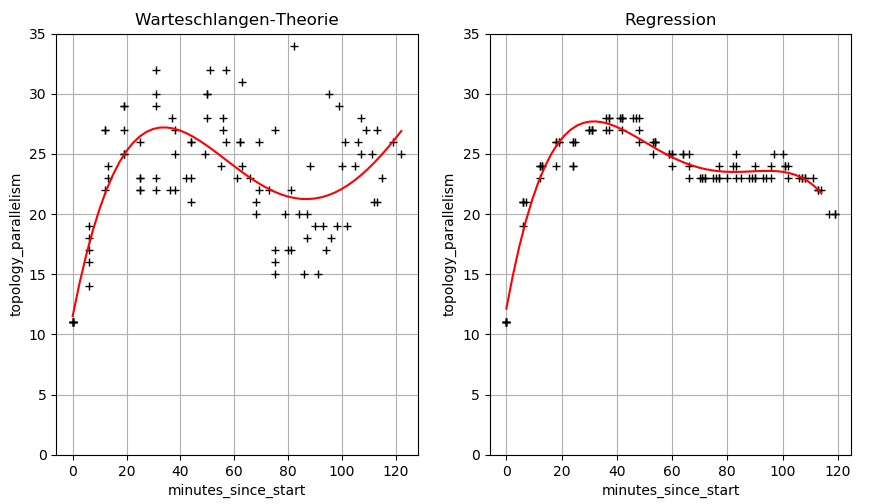
\includegraphics[scale=0.65]{Parallelisierung}
\caption{Parallelisierungsgrade während der Evaluation.}
\end{figure}

\subsection{Latenz der Tupel}

Wenn man den Verlauf der Tupel-Latenz in Abbildung 9.4 betrachtet, kann man feststellen, dass diese sich gegenläufig zum Verlauf des Parallelisierungsgrades verhalten.
Auffällig ist auch, dass die Messwerte von WT im Schnitt deutlich niederer sind, als die Messwerte von RG.

Dies ist durch mehrere Ursachen zu erklären.
Zum einen wird die Topologie wesentlich häufiger durch WT angepasst, als es bei RG der Fall ist.
Wird die Topologie wieder gestartet ist der Fluss der Tupel ungehemmter, als wenn sie konstant läuft.
Dieser Effekt wurde versucht damit abzufangen, dass immer nur die letzten drei Minuten des fünf Minuten Intervalls gemessen wurden.
Trotzdem kann sich der Effekt auf die Latenzen auswirken, da die Topologie eventuell länger als zwei Minuten benötigt bis sie einen stabilen Zustand erreicht.
Des Weiteren ist WT speziell dafür entwickelt die Latenz der Tupel unter einen gewissen Grenzwert zu halten, sodass dies ein essentieller Bestandteil der Steuerung ist.

Jedoch ist festzustellen, dass der gesetzte Maximalwert von zehn Millisekunden für die Latenz des Pfades von WT nicht eingehalten wurde.
Der Grund dafür ist, dass die Berücksichtigung der gemessenen Latenz des Kanals für die Evaluation nicht aktiviert war.
Somit wird die Netzwerklatenz und die reale Warteschlange vor dem Operator nicht berücksichtigt und die berechnete Wartezeit nicht über den Koeffizienten \(e\) angepasst.

Dass der Latenzwert bei RT vergleichsweise hoch ist, könnte daran liegen, dass das Modell eines Operators schlechte Vorhersagen getroffen hat.
Dieser Operator erzeugt dann einen Flaschenhals der die Latenz des Tupels stark erhöht.

Dass die Latenz am Schluss der Evaluation von RT stark ansteigt, könnte daran liegen, dass die Trainingsdaten einen Abfall der eingehenden Tupel gegen Ende aufweisen und deshalb der Parallelisierungsgrad geändert wird.
Diese Struktur der Trainingsdaten wäre damit zu erklären, dass durch die vielen Umstellungen durch WT die Topologie oft gestoppt wird und so über lange Zeit nur die Lesegeschwindigkeit die Ausgabe der Tupel von der Quelle beschränkt.
Dies führt zu hohen Spitzenwerten für die Anzahl ankommender Tupel.
Gegen Ende der Evaluation ist der Verlauf von WT aber weniger schwankend und die Spitzenwerte für ankommende Tupel sinken.
Somit sinkt auch in den Trainingsdaten die Anzahl ankommender Tupel gegen Ende der Evaluation, was den Effekt erklären könnte.

\begin{figure}
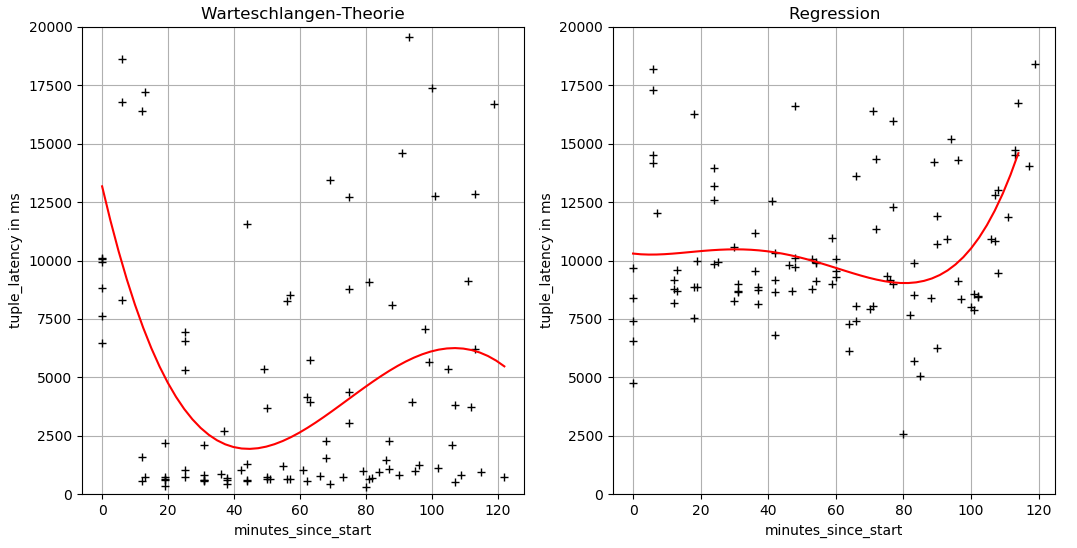
\includegraphics[scale=0.55]{Latenz}
\caption{Latenz der Tupel während der Evaluation.}
\end{figure}

\subsection{Tupel-Fehlerrate}

Zuletzt soll noch die Fehlerrate der Tupel betrachtet werden.
Die Fehlerrate berechnet sich aus dem Verhältnis der Anzahl Tupel, deren Verarbeitung fehlgeschlagen ist, und der Anzahl Tupel, deren Verarbeitung erfolgreich war.
Ein Tupel wird von der Topologie als fehlgeschlagen gewertet, wenn es innerhalb von 60 Sekunden nicht erfolgreich verarbeitet wurde.
In beiden Diagrammen der Abbildung 9.5 ist deutlich zu sehen, dass die Fehlerrate zu Beginn sehr hoch ist.
Erst wenn die Operatoren ausreichend skaliert sind, stabilisiert sich die Fehlerrate.
Für WT ist zu sehen, dass die Fehlerrate sehr oft nahe bei 0\% liegt.
Dies ist dadurch erklärbar, dass fehlerhafte Tupel erneut von der Quelle ausgegeben werden.
Der Algorithmus reagiert anschließend stark auf die erhöhte Anzahl ausgegebener Tupel und kann den Überschuss kurzfristig ausgleichen.
Diese Verhalten wurde in Kapitel 9.7.1 bereits beschrieben.

RG weist hingegen eine sehr hohe Fehlerrate auf.
Dies kann darauf zurückgeführt werden, dass der Algorithmus langfristige Prognosen betrachtet und die erneut gesendeten Tupel nicht kurzfristig ausgleicht.
Zudem basieren die Prognosen auf Messwerten von WT.
WT gleicht die Fehlerrate kurzfristig aus.
Da RG aber auf einem Mittelwert der gemessenen Werte basiert, können diese Spitzen nicht abgefangen werden.

Die hohe Fehlerrate erklärt ebenfalls warum die Latenz der Tupel unter RG in der zweiten Hälfte konstant hoch bleibt.
Im Vergleich zu WT beleibt der Parallelisierungsgrad von RG in der zweiten Stunde konstant und ist somit höher als bei WT.
Allerdings ist die Latenz der Tupel unter RG dennoch höher als bei WT.
Dies erklärt sich durch die konstant hohe Fehlerrate, die nicht abgearbeitet werden kann und somit die Operatoren mit erneut gesendeten Tupeln dauerhaft stark belastet.

\begin{figure}
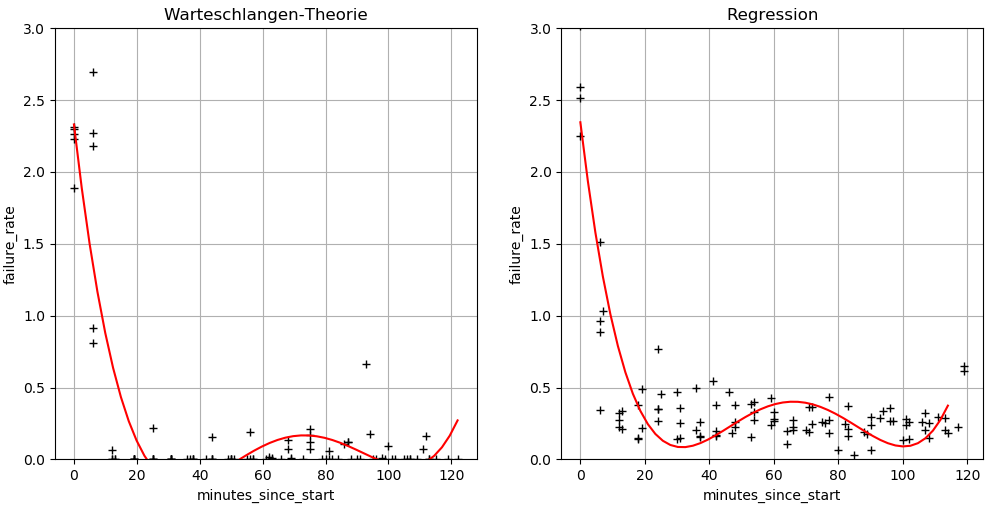
\includegraphics[scale=0.55]{Fehlerrate.PNG}
\caption{Fehlerrate der Tupel während der Evaluation.}
\end{figure}

\subsection{Schlussfolgerungen}

Für das in der Evaluation verwendete Muster des Arbeitsaufwands scheint WT besser geeignet zu sein.
Die Latenz und die Fehlerrate sind beide niedriger als bei RG.
Allerdings benötigt WT zeitweise mehr Ressourcen, die zur Verfügung stehen müssen.
Im Mittel sind die Kosten für Operatoren der Topologie ähnlich.

Da durch die zeitliche Komporession der Daten die Spitzen und Tiefen schneller aufeinander folgen, ist es erklärbar, dass WT durch die eher kurzfristige reaktive Herangehensweise besser auf die schnelle Abfolge der Extreme reagieren kann.
Dies setzt allerdings voraus, dass die ankommenden Tupel während der häufigen Änderungen der Topologie zwischengespeichert werden können.
Der Algorithmus von Lohrmann et al. konnte, trotz vielen Änderungen an der Topologie, den Rückstand, der Tupeln die bearbeitet werden müssen, ausgleichen.

Der Algorithmus von Zacheilas et al. ist relativ stark an die Mittelwerte der Trainingsdaten gebunden.
Damit der Algorithmus erfolgreich eingesetzt werden kann, ist es notwendig, dass Messdaten für möglichst viele Parallelisierungsgrade eines Operators vorhanden sind.
Sind die Daten nicht vorhanden, dann unterscheiden sich die Vorhersagen für hohe und niedere Parallelisierungsgrade nicht stark genug.
Durch eine Optimierung der Hyperparameter kann diesem Verhalten ebenfalls entgegengewirkt werden.

Ein weiterer Punkt ist, dass RG den letzten Operator der Topologie nie skalieren wird, da die Anzahl der ausgegebenen Tupel immer null entspricht.
Somit ist die Anzahl verpasster Tupel des Operators und die damit verbundenen Kosten immer null.

Für einen Workload der wenige Ausreisser besitzt und sich eher moderat verändert wäre der Algorithmus von Zacheilas et al. vermutlich besser geeignet als der Algorithmus mit Warteschlangen-Theorie. 


%\input{...weitere Kapitel...}
% !TeX spellcheck = de_DE

\chapter{Zusammenfassung und Ausblick}\label{chap:zusfas}
In der vorliegenden Arbeit wurde zuerst die Grundlage für das Skalieren von Operatoren in CEP-Topologien erläutert.
Um den Parallelisierungsgrad der Operatoren zu steuern, wurden in den letzten Jahren mehrere Algorithmen vorgeschlagen.
Verschiedene Algorithmen wurden betrachtet und deren Stärken und Schwächen analyisert.
Anschließend wurden zwei Algorithmen gewählt die implementiert und ausgiebig evaluiert werden sollen.

Für die Implementation der Algorithmen wird ein Framework erstellt, welches es erlaubt dass diese Algorithmen unabhängig vom gesteuerten CEP-System arbeiten könne.
Das Framework bietet als Schnittstelle für die Algorithmen ein Graph-Modell, das die Werte der Topologie autonom ausliest und bereitstellt.
Das Graph-Modell ermöglicht es neue Algorithmen zu implementieren, ohne dass diese sich mit der Beschaffung von Messdaten aus den CEP-Systemen befassen müssen.
Damit das Framework universell einsetzbar ist, muss für das entsprechende CEP-System ein Adapter implementiert werden.
Der Adapter muss dabei die Spezifika des CEP-Systems kapseln und eine REST-Schnittstelle für das Framework bereitstellen.
Um die Algorithmen auf dem CEP-System Heron evaluieren zu können, wurde ein bestehender Adapter für Heron so erweitert, dass er alle benötigten Funktionen bereitstellt.

Anschließend wurden die beiden Algorithmen implementiert.
Dabei wurden zum Teil leichte Modifikationen unternommen um sie robuster und flexibler zu machen.
Einer der Algorithmen wurde von Lohrmann et al. vorgeschlagen und basiert auf der Verwendung der Warteschlangentheorie.
Er verwendet das Modell, dass Tupel vor einem Operator warten müssen, bis sie verarbeitet werden.
Der Algorithmus versucht die Wartezeit von Tupeln über das Skalieren von Operatoren unter einen benutzerdefinierten Grenzwert zu senken
Der zweite Algorithmus basiert auf Vorhersagen über den zukünftigen Zustand der Topologie und wurde von Zacheilas et al. vorgeschlagen.
Die Vorhersagen werden mit Hilfe von maschinellem Lernen getroffen.
Anschließend werden die Vorhersagen mit einer Kostenfunktion gewichtet und in einen Graph von Zustandsübergängen modelliert.
Der kürzeste Pfad durch den Graph bestimmt anschließend den nächsten Parallelisierungsgrad des Operators.

Zuletzt wurde ein Test-Cluster mit Heron aufgebaut, um die Algorithmen zu evaluieren.
Für die Evaluation wurden eine Menge von Daten benötigt, die eine Topologie auslasten kann.
Deshalb wurden über eine Woche Daten von der Twitter Streaming API ausgelesen.
Außerdem wurde eine Topologie implementiert, die Twitter-Daten analysiert und für die Evaluation eingesetzt wurde.
Während der Evaluation mussten die Algorithmen die implementierte Topologie steuern, während diese die gesammelten Daten innerhalb von zwei Stunden verarbeitete.
Dabei wurden verschiedene Messwerte erhoben und gegenüber gestellt.
Das Ergebnis war, dass der Algorithmus von Lohrmann et al. für das Verhaltensmuster der verarbeiteten Daten deutlich bessere Werte für Tupel-Latenz und Fehlerrate erzielte.
Die Erklärung dafür liegt darin, dass der Operator reaktiv auf Schwankungen in der Topologie reagiert.
Der Algorithmus von Zacheilas et al. hält den Parallelisierungsgrad der Operatoren eher konstant und gleicht kurzfristige Schwankungen nicht aus.
Er ist daher besser für einen sich stetig ändernden Arbeitsaufwand mit wenig Minima und Maxima geeignet.

\section*{Ausblick}

Neben der durchgeführten Evaluation sollten noch weitere Evaluationen mit den implementierten Algorithmen durchgeführt werden.
Die Parameter dabei sind sehr vielfältig.
Zum einen könnte die Rate, mit der die Quelle Tupel ausgibt, angepasst werden.
Ebenso kann das Zeitfenster für das Erfassen der Messwerte und deren Überprüfung durch den Algorithmus verändert werden.
Da in der Evaluation nur drei Minuten des fünf minütigen Zeitfensters betrachtet werden, wäre es interessant wie sich der Zustand direkt nach dem Skalieren auf die evaluierten Messwerte auswirkt.
Interessant wäre ebenfalls ein andere Daten oder ein anderes Muster des anfallenden Arbeitsaufwandes zu testen.

Außerdem kann die Konfiguration von Heron angepasst werden, sodass mehr Tupel in den Buffer vor den Operatoren geladen werden können.
Diese Änderung würde sich auf die Anzahl fehlgeschlagener Tupel auswirken.
Ebenso könnte die Konfiguration der Topologie abgewandelt werden.
Wenn die Topologie mit der ''AT\_MOST\_ONCE'' Garantie konfiguriert wird, werden fehlerhafte Tupel nicht mehr wiederholt,
was die Last der Operatoren deutlich verringern könnte.
Ein weiterer interessanter Punkt wäre zu sehen, wie sich die Messwerte der Algorithmen verhalten wenn die Drosselung des Tupel-Stroms in der Topologie aktiviert ist.

Ein weiterer Punkt ist die Optimierung der Trainigsdaten für die Vorhersage.
Mit einem größeren Datensatz könnte der Algorithmus von Zacheilas et al. exaktere Vorhersagen treffen und somit besser agieren.
Hier spielen auch die Hyperparamter eine große Rolle.
Diese wurden für die vorliegende Evaluation nicht optimiert.
Die Qualität der Vorhersagen würde sich auch mit den aktuellen Trainingsdaten verbessern lassen, wenn das jeweilige Optimum der Hyperparameter berechnet wurde.

Desweiteren könnte das Framework so erweitert werden, dass es möglich ist weitere CEP-Systeme zu steuern.
Momentan ist nur der Adapter für Heron verfügbar.
Die Erweiterung würde es ermöglichen die Algorithmen auf anderen Systemen zu testen.
Die Möglichkeit noch mehr verschiedene Algorithmen miteinander zu vergleichen sollte ebenfalls in Betracht gezogen werden.
Das Framework stellt das Graph-Modell als Grundlage bereit, sodass neue Algorithmen mit weniger Aufwand implementiert werden können.

%
%
%\renewcommand{\appendixtocname}{Anhang}
%\renewcommand{\appendixname}{Anhang}
%\renewcommand{\appendixpagename}{Anhang}
\appendix

\clearpage

%\printindex

\printbibliography

\ifdeutsch
Alle URLs wurden zuletzt am 14.\,10.\,2018 geprüft.
\else
All links were last followed on March 17, 2008.
\fi

\pagestyle{empty}
\renewcommand*{\chapterpagestyle}{empty}
\Versicherung
\end{document}
